\chapter{Fit validation}
\label{ch:appendix_toys}

This appendix details the fit validations studies performed for the frameworks described in Chapters~\ref{ch:B2DsKK} and~\ref{ch:B2DsPhi}. 

\section{Fit validation for the \decay{\Bp}{\Dsp\Kp\Km} fitting framework}
\label{sec:app_toys_B2DsKK}


The \decay{\Bp}{\Dsp\Kp\Km} fitting framework is validated by generating pseudo-experiment datasets and fitting them with the PDF model. The free parameters are treated using the plug-in method~\cite{plugin}; the generated values of all free parameters are \emph{plugged in} from the best fit to data.      

The fitted values and uncertainties are determined for each pseudo-experiment and a corresponding pull determined, defined as
\begin{equation}
g_{\text{pull}} = \frac{x_{\text{fit}} - x_{\text{gen}} }{\sigma}
\end{equation}
where $x_{\text{gen}}$ and $x_{\text{fit}}$ are the generated and fitted values of the variable, and $\sigma$ is the parameter's uncertainty.
For an ideal unbiased fit model, the pull of each parameter of interest would be normally distributed with unit width and mean of zero.  


%%%%%%%%%%%%%%%%%%%%%%%%%%%%%%%%%%%%%%%%%%%%%%%%%%%%%%%%%%
\begin{figure}[!h]
   \centering
   \begin{subfigure}[t]{1.0\textwidth}
      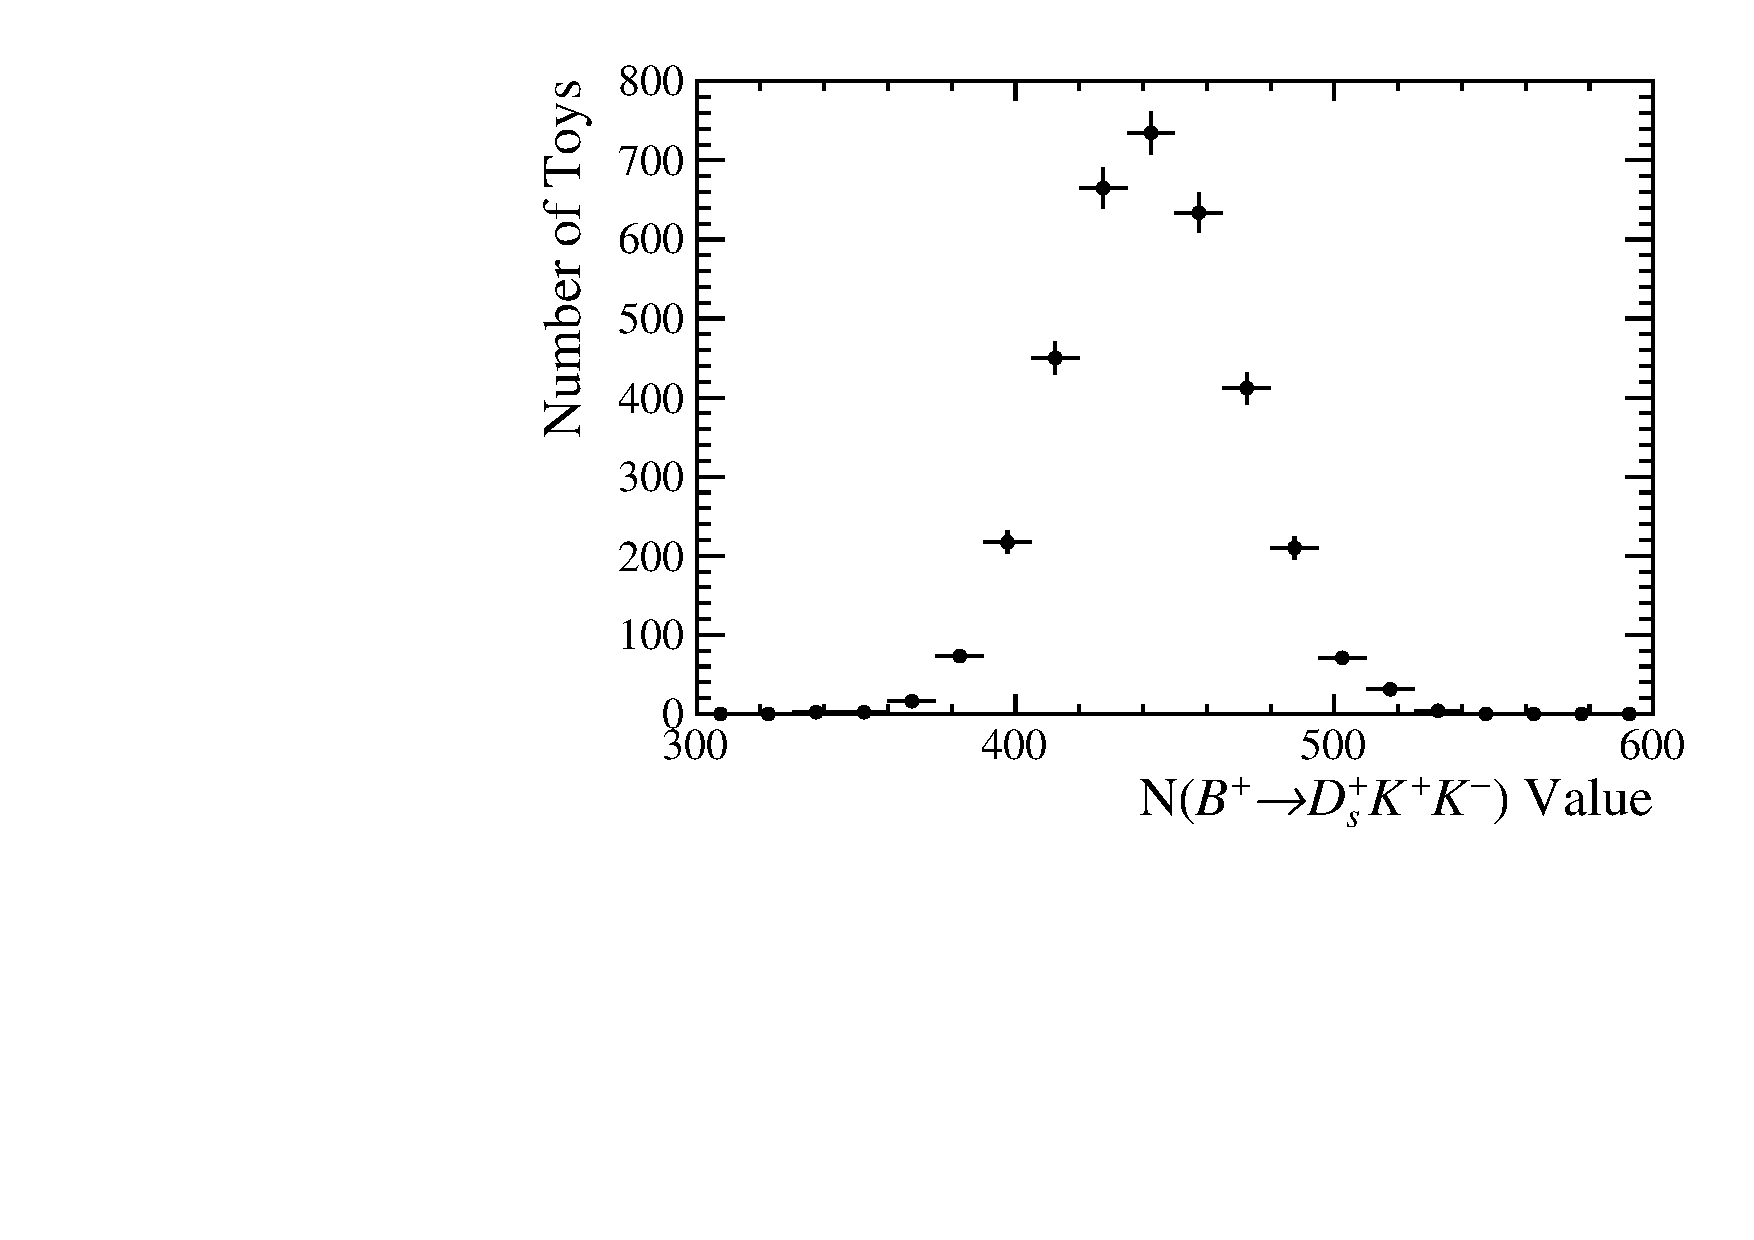
\includegraphics[width=0.32\textwidth]{figs/B2DsKK/Plots_DsKK_nsig_val.pdf}
      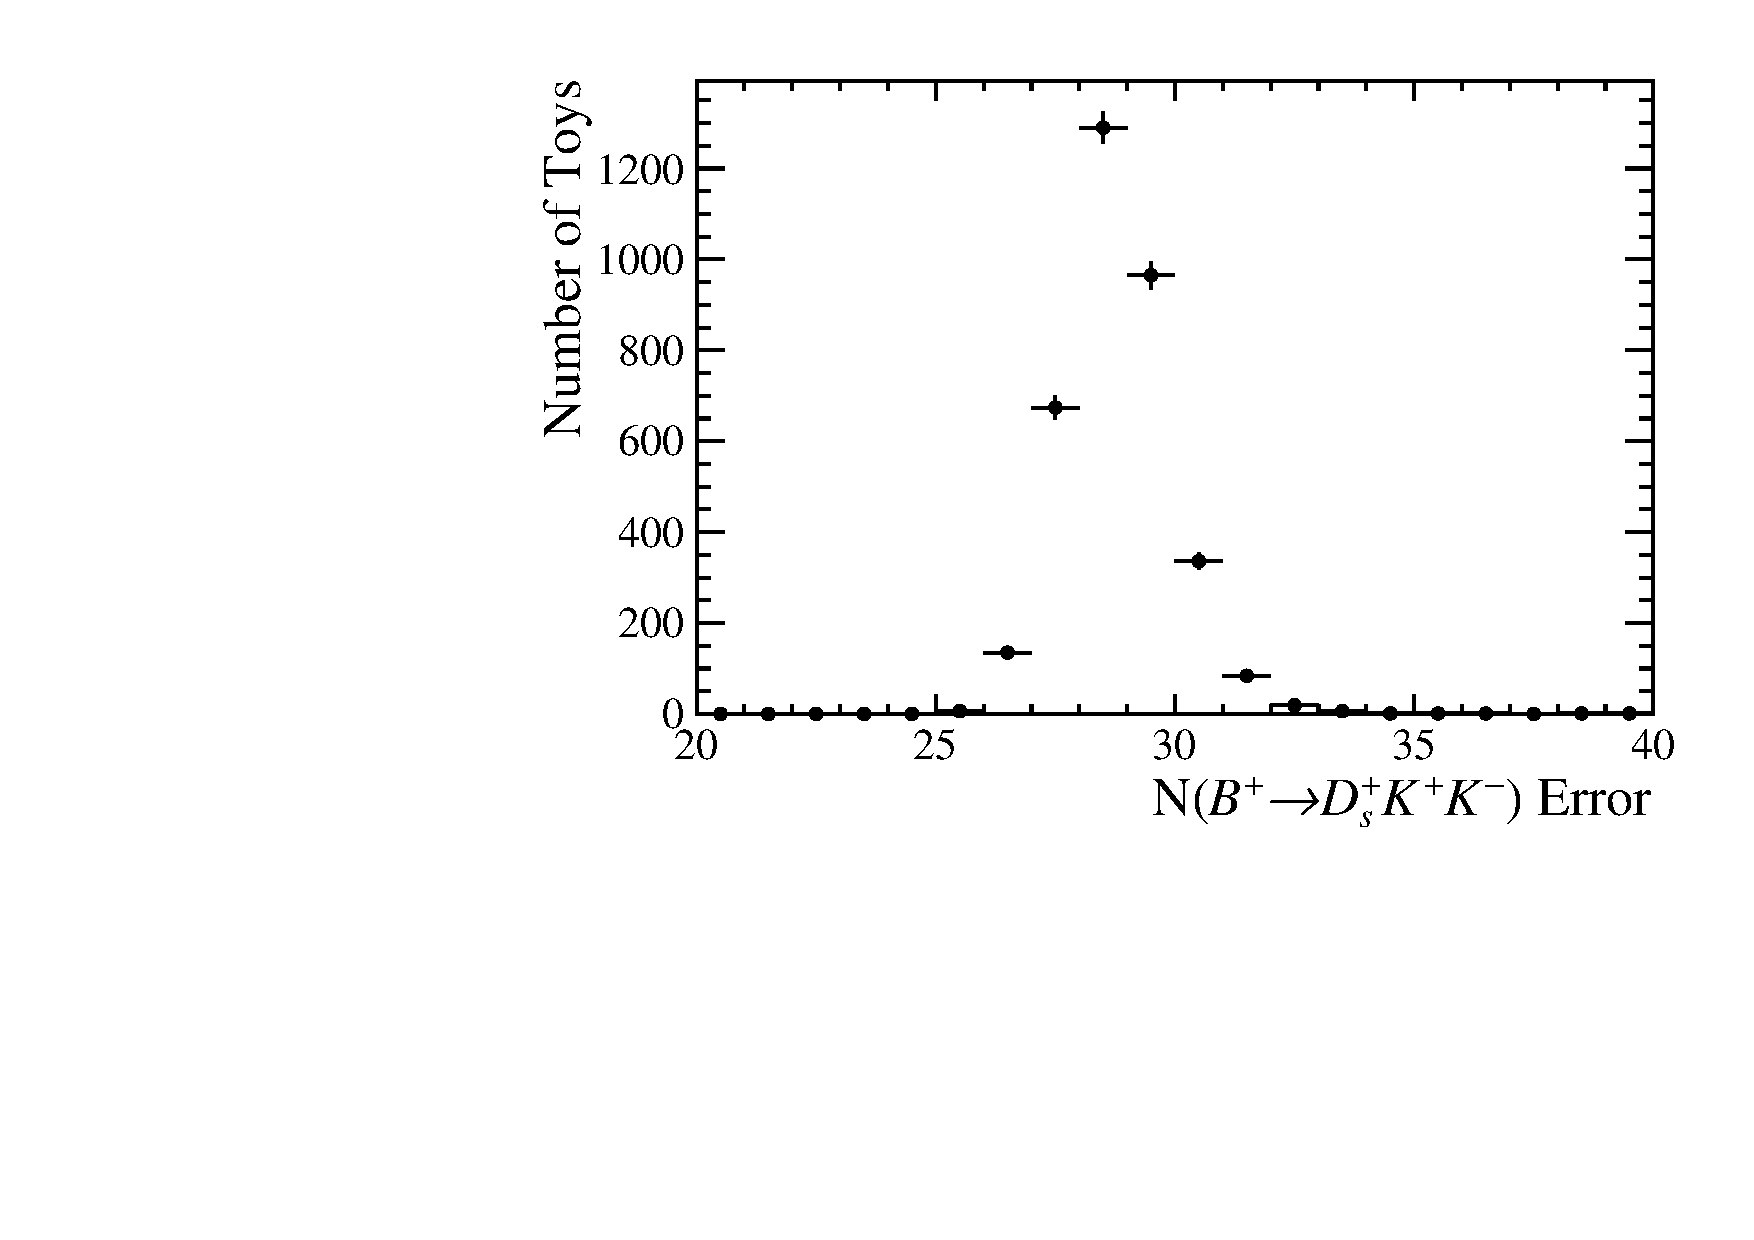
\includegraphics[width=0.32\textwidth]{figs/B2DsKK/Plots_DsKK_nsig_err.pdf}
      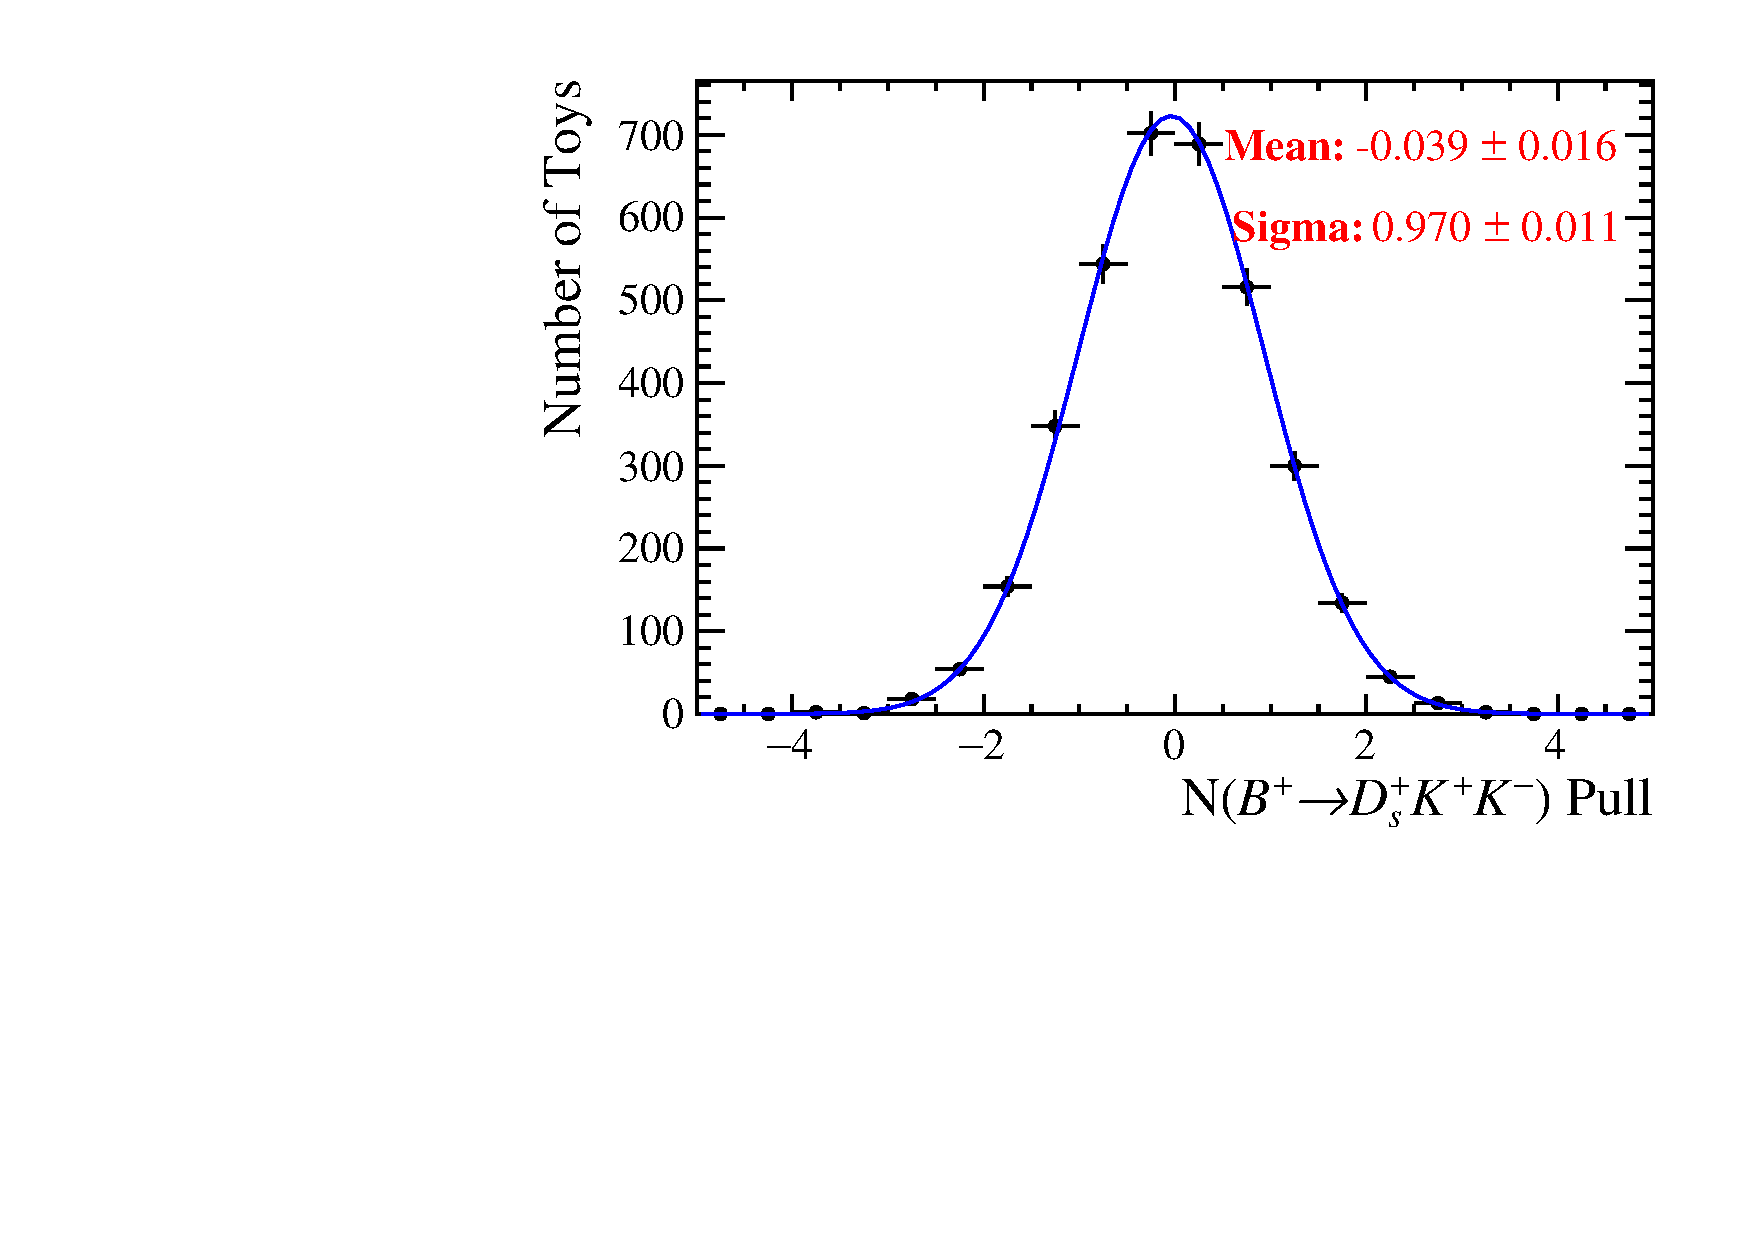
\includegraphics[width=0.32\textwidth]{figs/B2DsKK/Plots_DsKK_nsig_pul.pdf}
      \caption{Signal fit}
   \end{subfigure}\\
   \begin{subfigure}[t]{1.0\textwidth}
      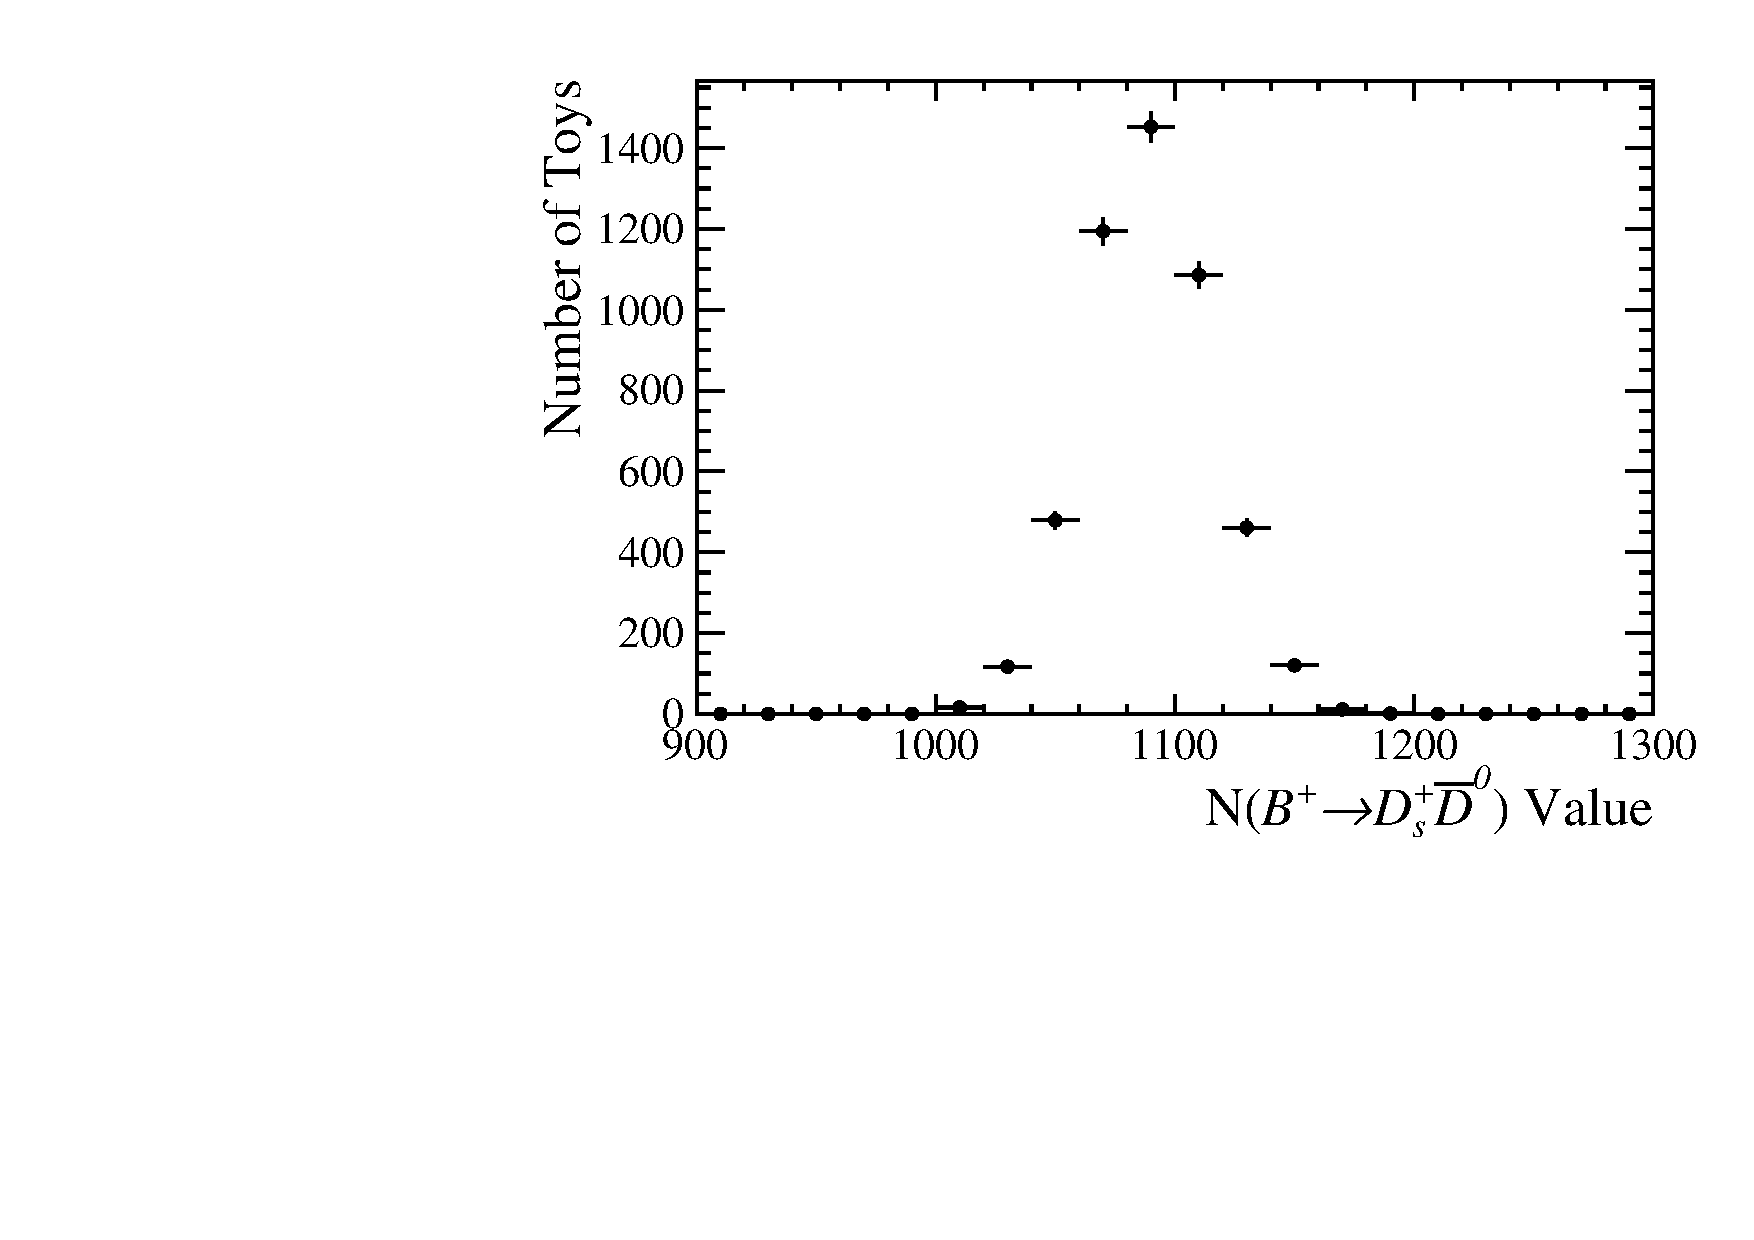
\includegraphics[width=0.32\textwidth]{figs/B2DsKK/Plots_DsD0_nsig_val.pdf}
      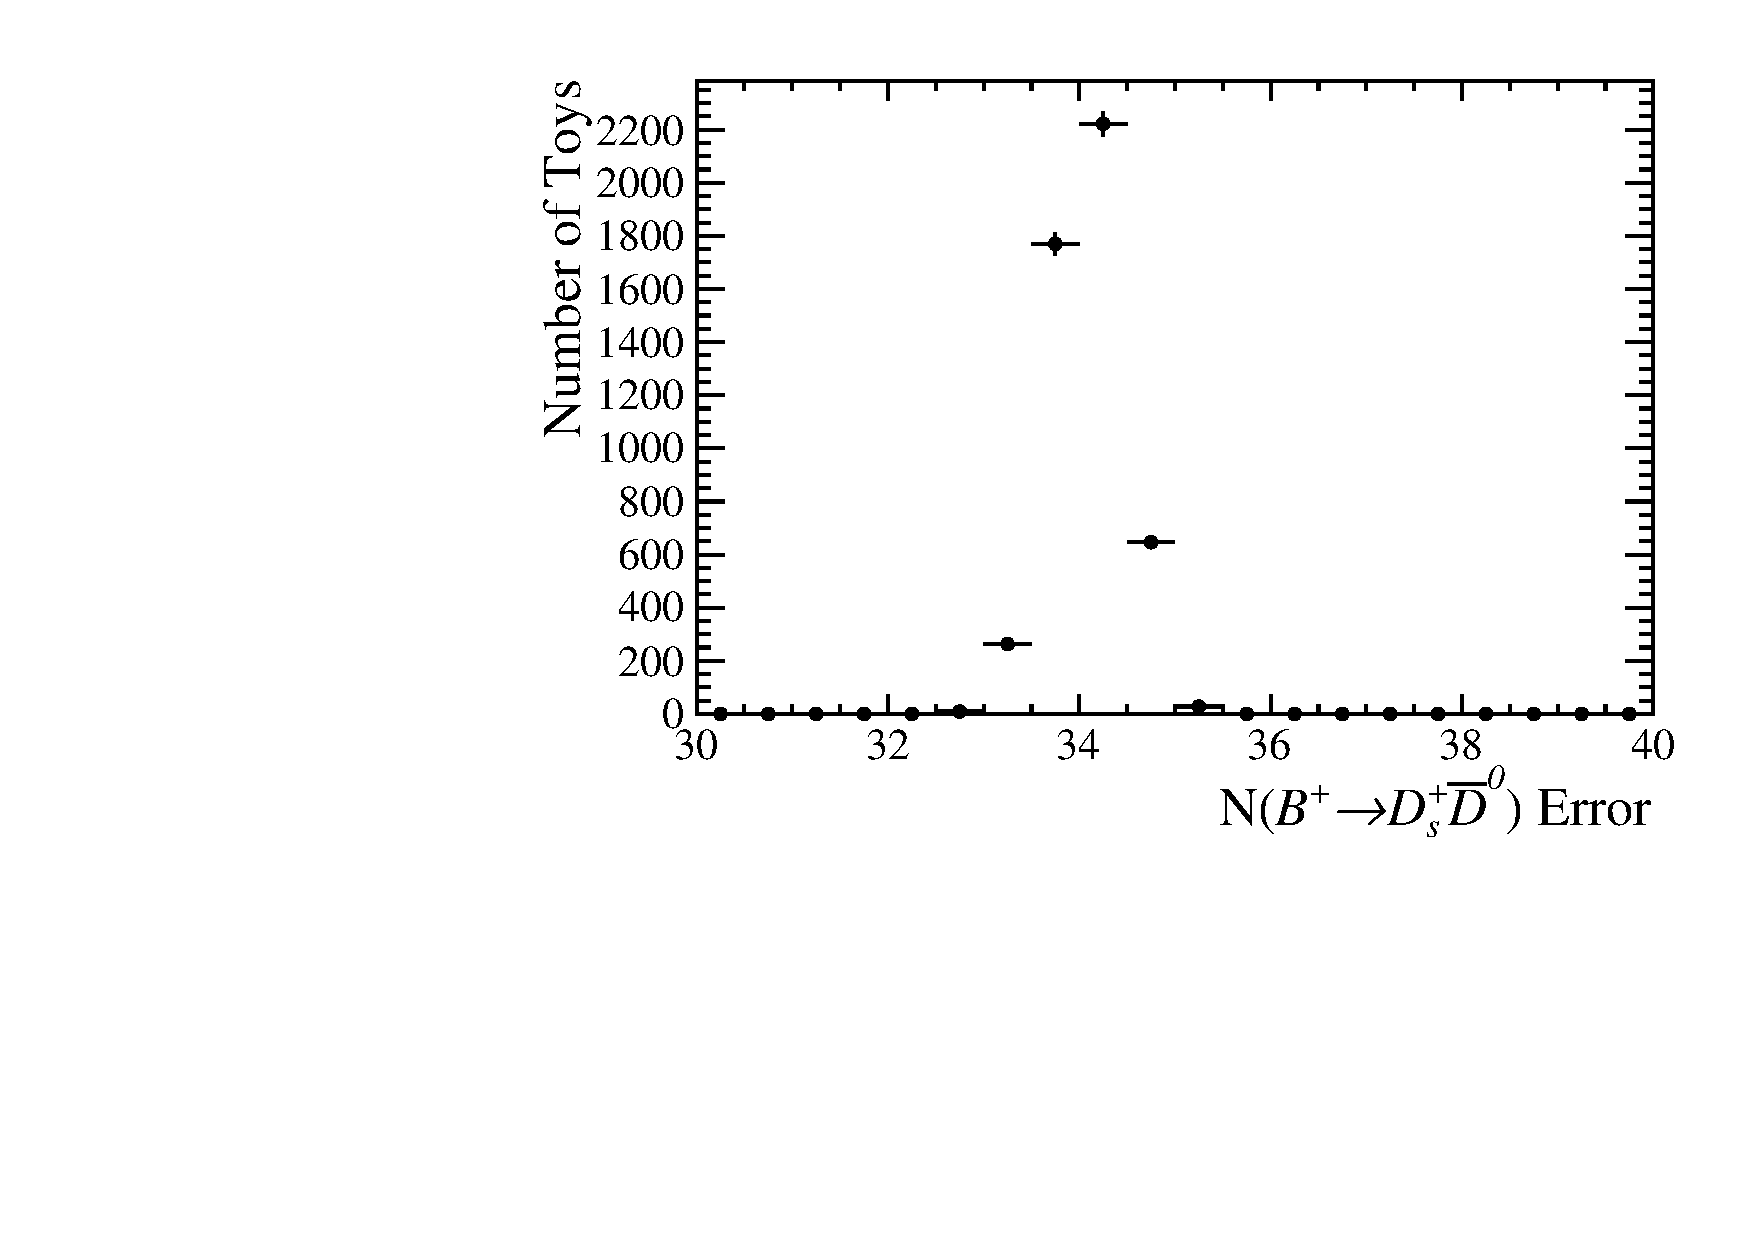
\includegraphics[width=0.32\textwidth]{figs/B2DsKK/Plots_DsD0_nsig_err.pdf}
      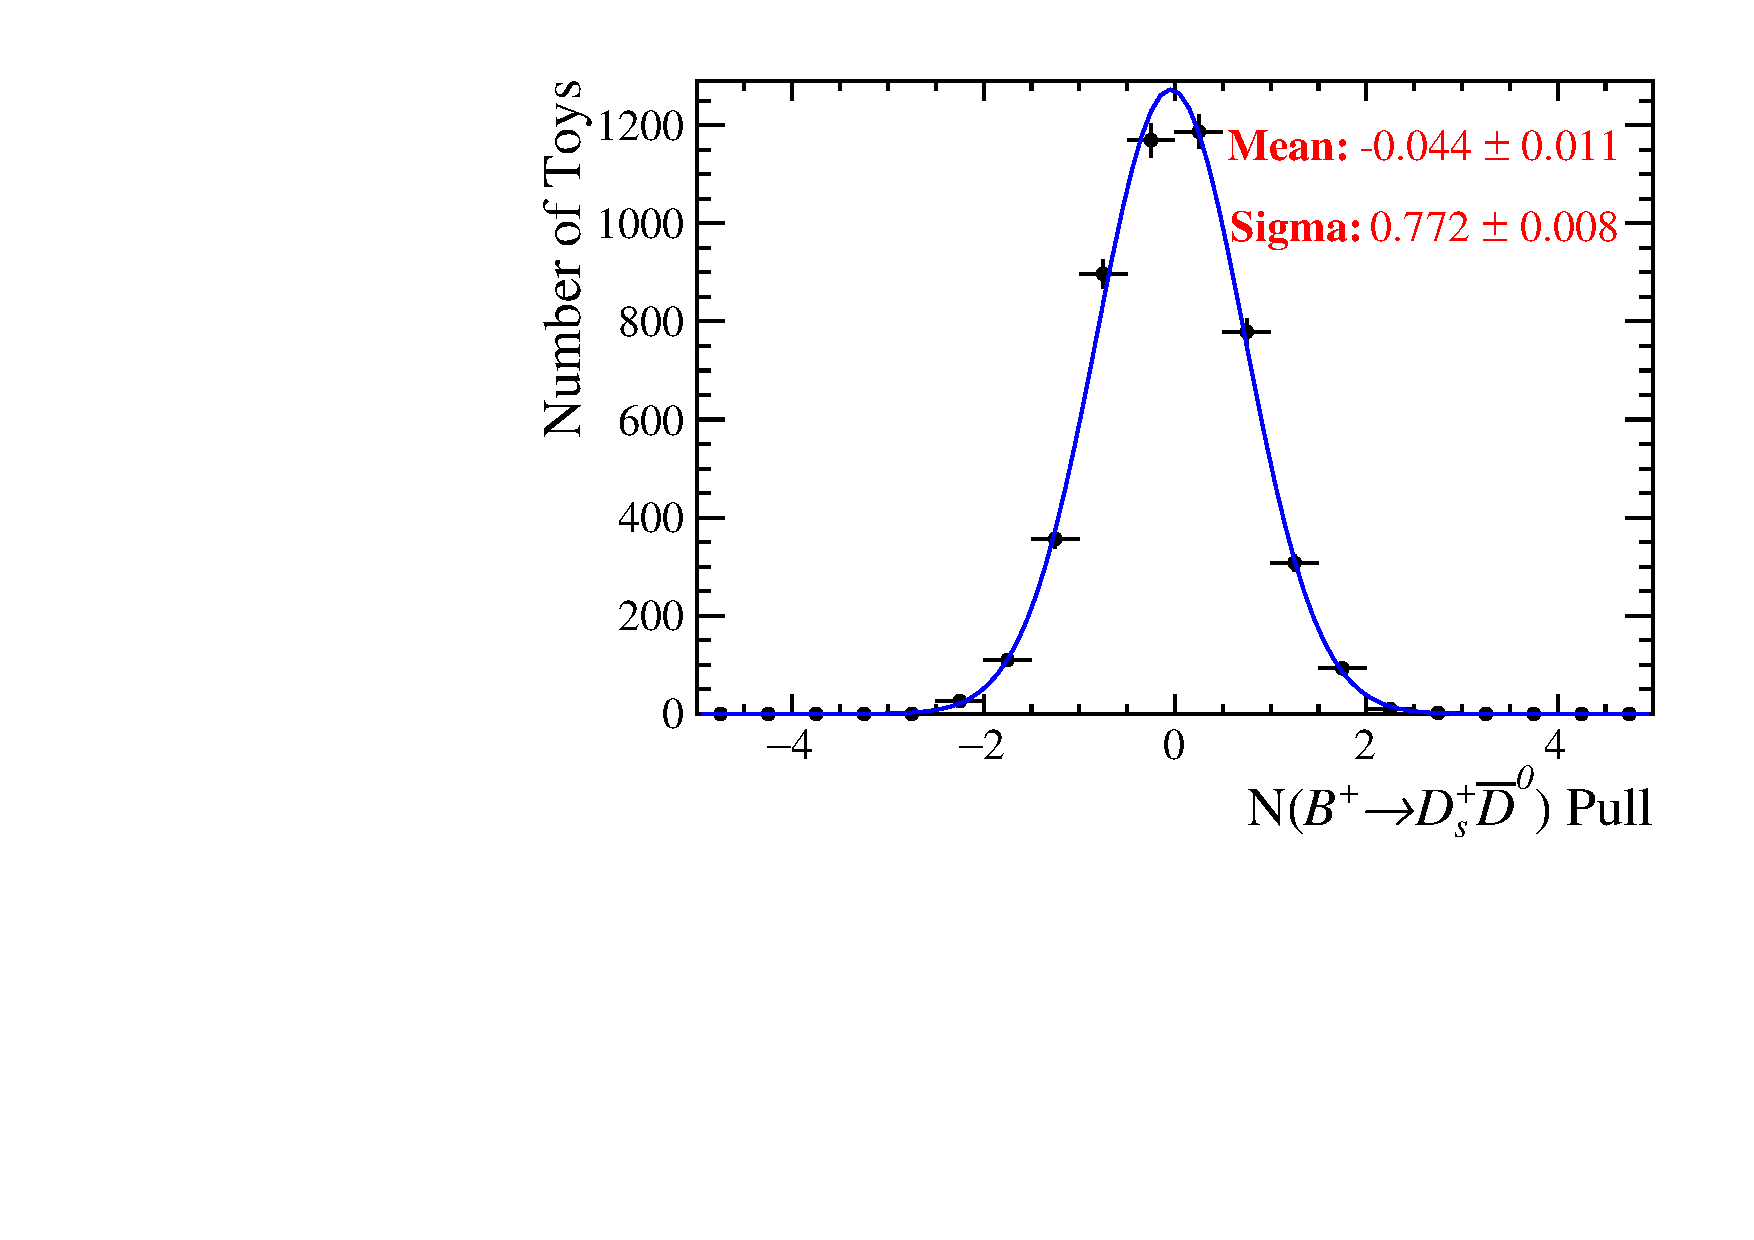
\includegraphics[width=0.32\textwidth]{figs/B2DsKK/Plots_DsD0_nsig_pul.pdf}
      \caption{Normalisation fit}
   \end{subfigure}\\
   \caption{The distribution of the signal and normalisation yields, errors and pulls as determined from pseudo-experiments. The result of fit performed to the pull distributions is overlaid in blue, along with the numerical results in red.}
   \label{fig:B2DsKK_Pulls}
\end{figure}
%%%%%%%%%%%%%%%%%%%%%%%%%%%%%%%%%%%%%%%%%%%%%%%%%%%%%%%%%%

The distributions of the yields, errors and pulls for the signal and normalisation pseudo-experiments are shown in Fig.~\ref{fig:B2DsKK_Pulls}. A fit is performed for each pull distributions using a Gaussian to determine the mean and width. 
For the signal yield the mean and width are within $3\sigma$ of zero and one respectively. The normalisation yield shows a significant bias in the width. The bias implies the fit model is overestimating the uncertainty $\sigma$ of the yield.
If the normalisation yield uncertainty dominates the uncertainty in the branching fraction this could lead to an overestimation of the uncertainty on the final measured branching fraction.

To determine how the normalisation uncertainty propagates to the branching fraction another set of pseudo-experiments are produced.
This set includes both signal and normalisation decays. To calculated the branching fraction the yield of \decay{\Bp}{\Dsp\Kp\Km} decays is corrected according to the signal efficiency as a function of the kinematics of a given candidate, as detailed previously in Eq.~\ref{eq:B2DsKK_corrected_yield}. The candidates are assumed to have a flat distribution in the two dimensional $m^{2}(\Kp\Km)$ vs. $m^{2}(\Dsp\Km)$ space used to parametrise the efficiency. The bias in the final branching fraction is much smaller than the bias normalisation pull.

\section{Fit validation for the \decay{\Bp}{\Dsp\phiz} fitting framework}
\label{sec:app_toys_B2DsPhi}

The simultaneous fitting framework is validated by generating pseudo-experiments. The total fit model PDF is randomly sampled to create a simulation sample with the same number of candidates as the nominal fit. These are then fitted using the same fit model, determining the best estimate and uncertainty of each parameter. The parameter values used to generate the pseudo-experiments are chosen to be the final parameter values as determined in a fit to data. This is known as the plug-in method~\cite{plugin}.
The fitted value and associated error is used to determine the pull of each parameter of interest. As the errors are determined asymmetrically using \minos the pull is defined conditionally to incorporate the appropriate error 
\begin{equation}
  g_{\text{pull}} = \left \{
  \begin{aligned}
    &\frac{x_{\text{gen}} - x_{\text{fit}} }{\sigma_{+}}, && \text{if}\ x_{\text{fit}} < x_{\text{gen}}\\
    &\frac{x_{\text{fit}} - x_{\text{gen}} }{\sigma_{-}}, && \text{otherwise},
  \end{aligned} \right.
\end{equation} 
where $x_{\text{fit}}$ and $x_{\text{gen}}$ are the fitted and generated values of the variable, and $\sigma_{+}$ and $\sigma_{-}$ are the high and low asymmetric errors.

The distributions of the values, errors and pulls for the yields of the normalisation decay in each of the \Dsp decays are shown in Fig.~\ref{fig:B2DsPhi_Pulls_normalisation}. The mean and widths are determined using simple fits to the pull distributions. The results and PDFs for these fits are overlaid on the distributions. The normalisation yield means and widths are found to be within $2\sigma$ of zero and one respectively.


%%%%%%%%%%%%%%%%%%%%%%%%%%%%%%%%%%%%%%%%%%%%%%%%%%%%%%%%%%
\begin{figure}[!h]
   \centering
   \begin{subfigure}[t]{1.0\textwidth}
      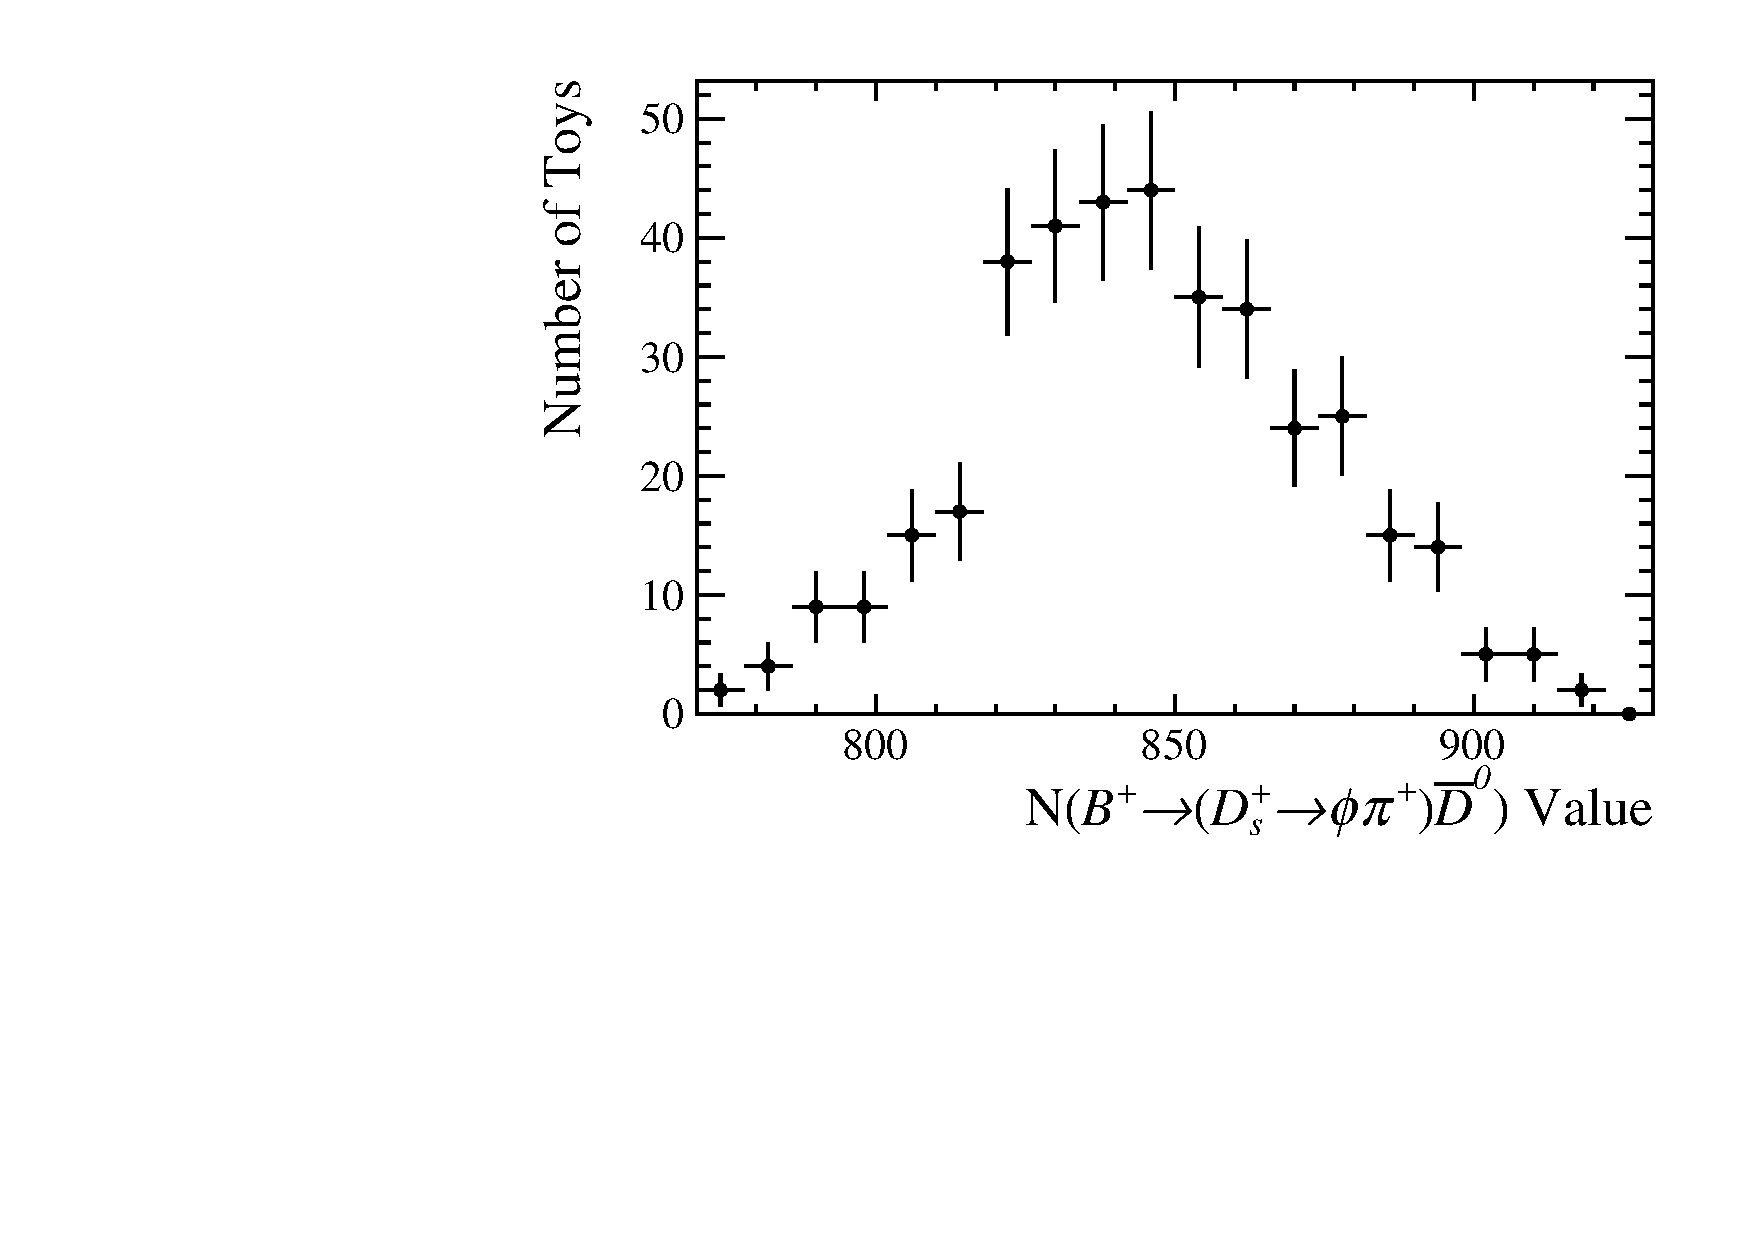
\includegraphics[width=0.32\textwidth]{figs/B2DsPhi/Plots_DsKK_Value_yield_peak_DsD0_Ds2PhiPi_toy_both_DsBDTbin1_PhiBDTbin1_both_both.pdf}
      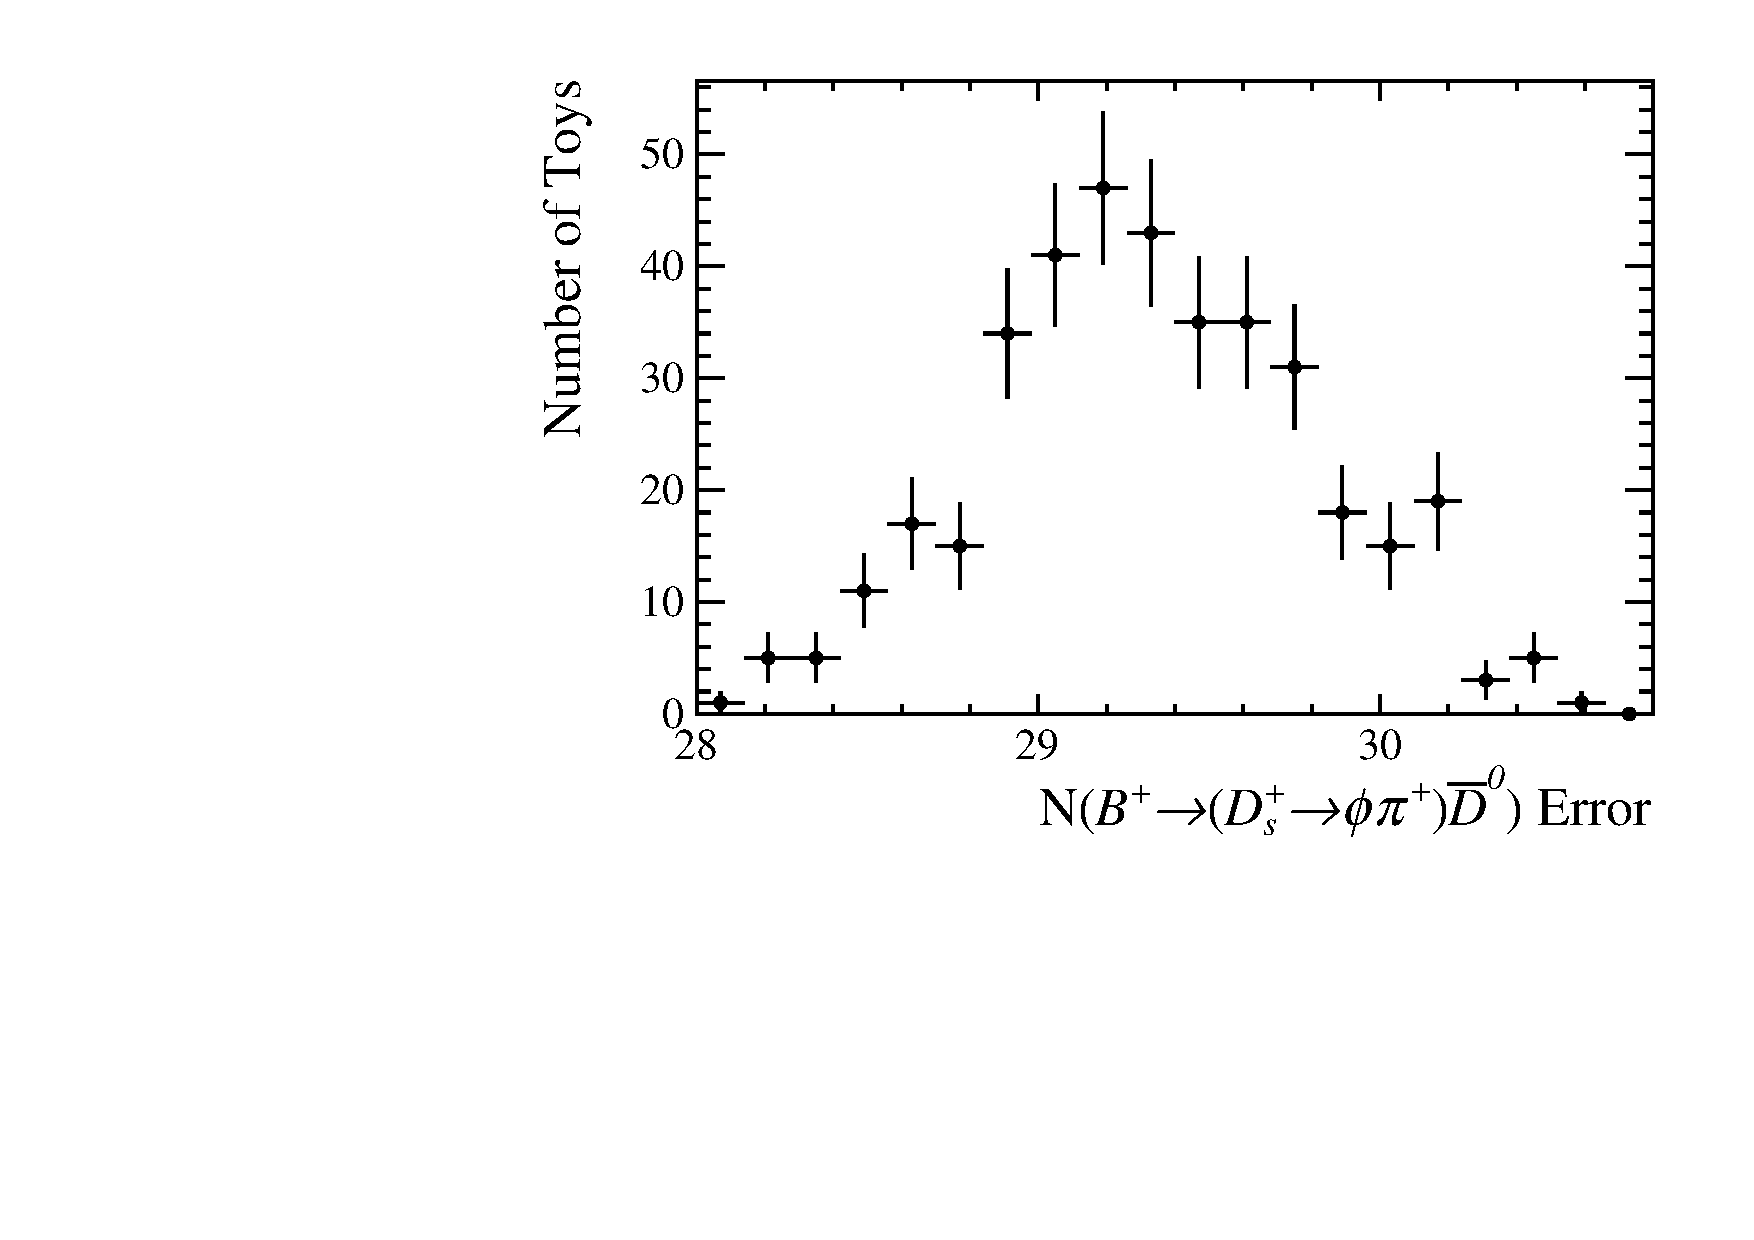
\includegraphics[width=0.32\textwidth]{figs/B2DsPhi/Plots_DsKK_Error_yield_peak_DsD0_Ds2PhiPi_toy_both_DsBDTbin1_PhiBDTbin1_both_both.pdf}
      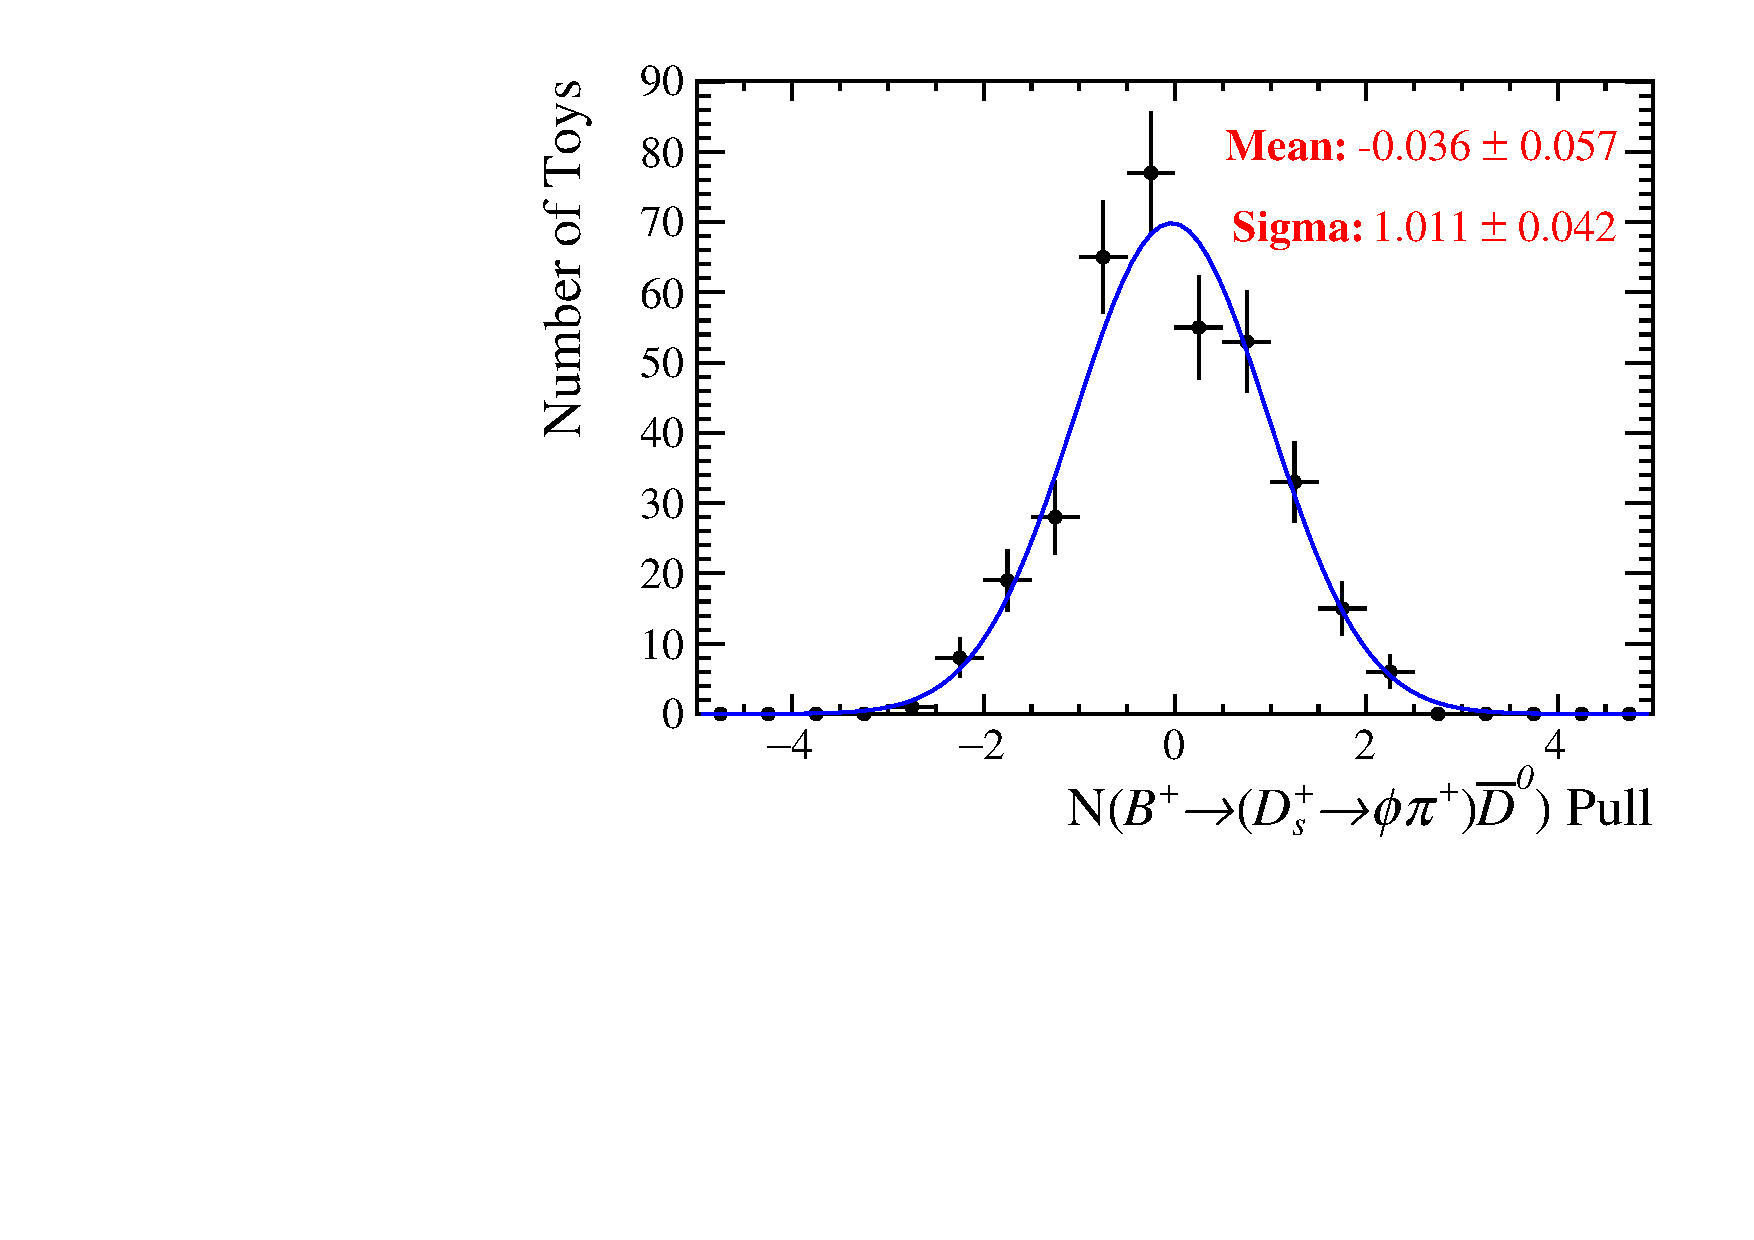
\includegraphics[width=0.32\textwidth]{figs/B2DsPhi/Plots_DsKK_Pull_yield_peak_DsD0_Ds2PhiPi_toy_both_DsBDTbin1_PhiBDTbin1_both_both.pdf}
      \caption{\decay{\Dsp}{\phiz\pip}}
   \end{subfigure}\\
   \begin{subfigure}[t]{1.0\textwidth}
      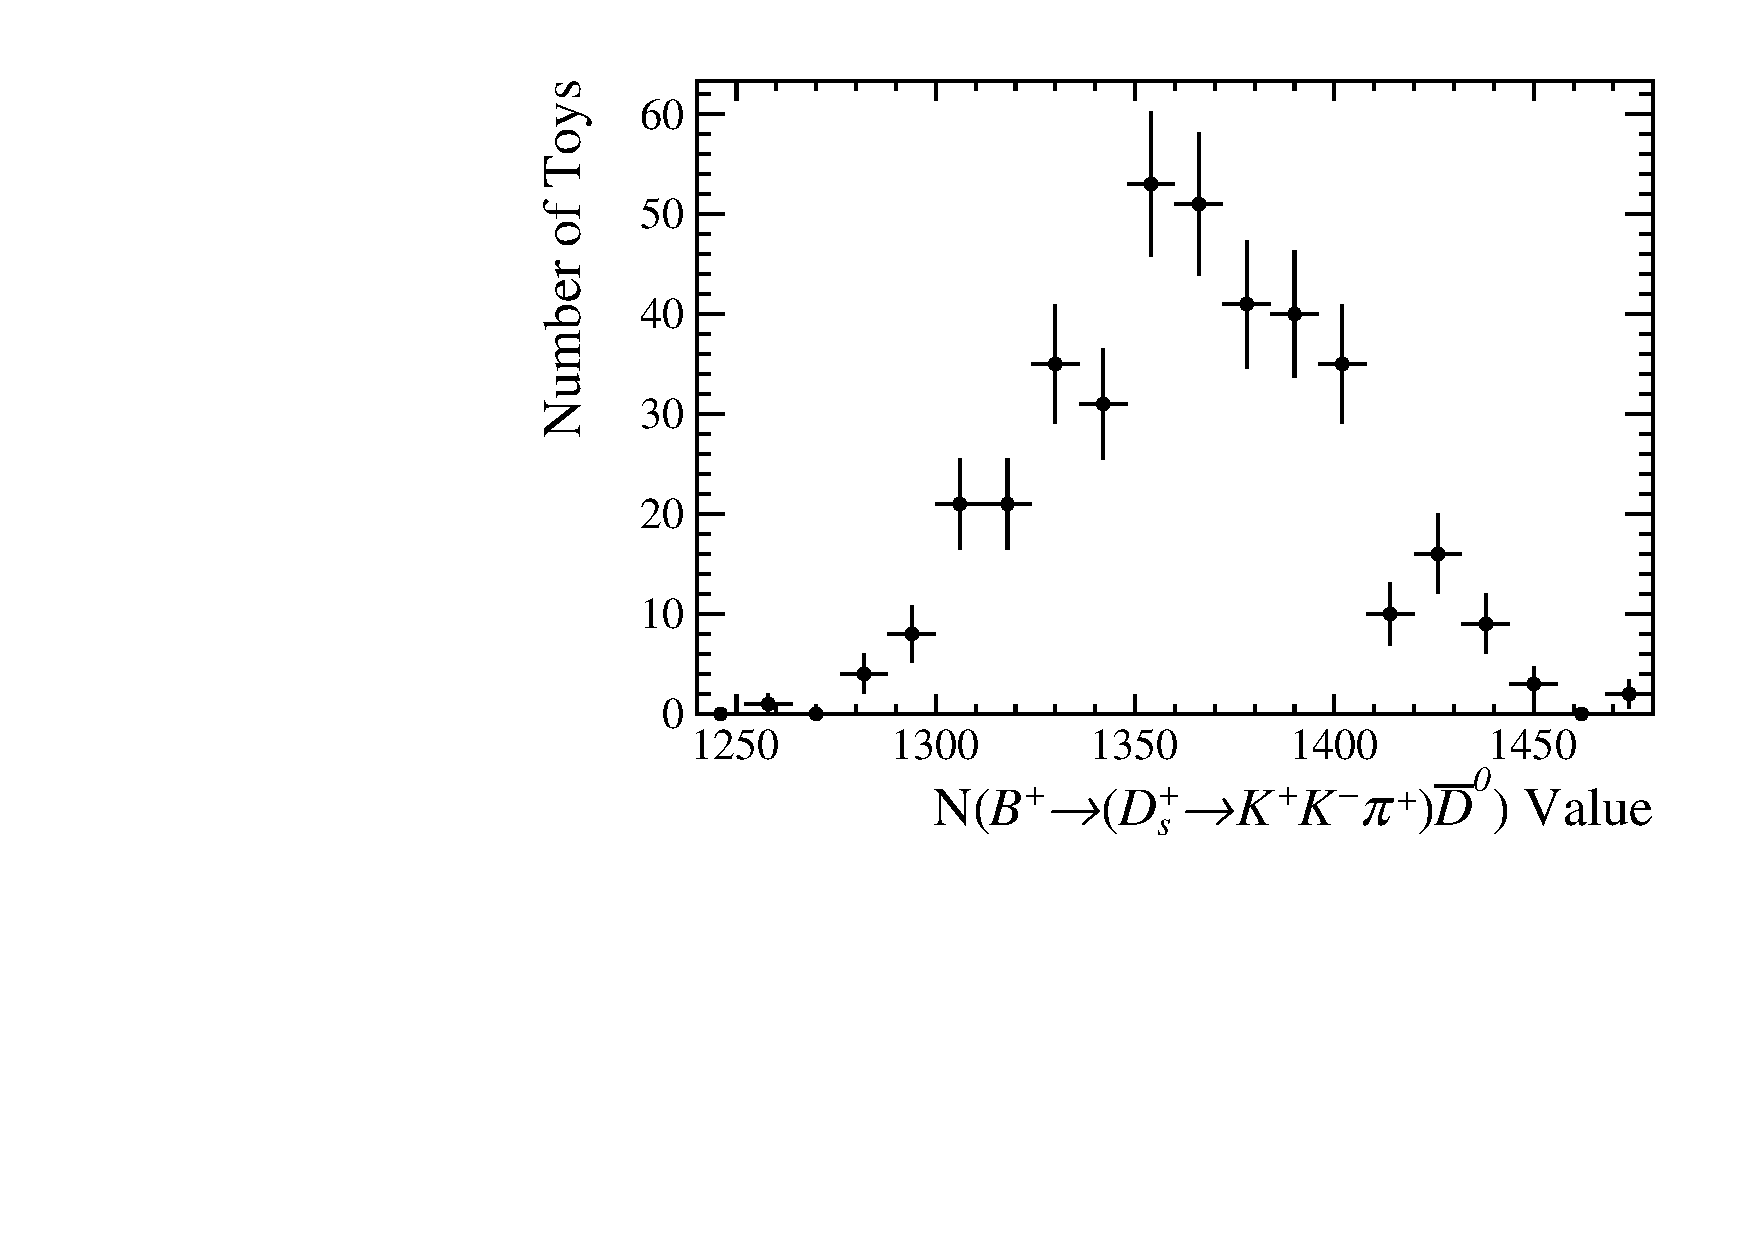
\includegraphics[width=0.32\textwidth]{figs/B2DsPhi/Plots_DsKK_Value_yield_peak_DsD0_Ds2KKPi_toy_both_DsBDTbin1_PhiBDTbin1_both_both.pdf}
      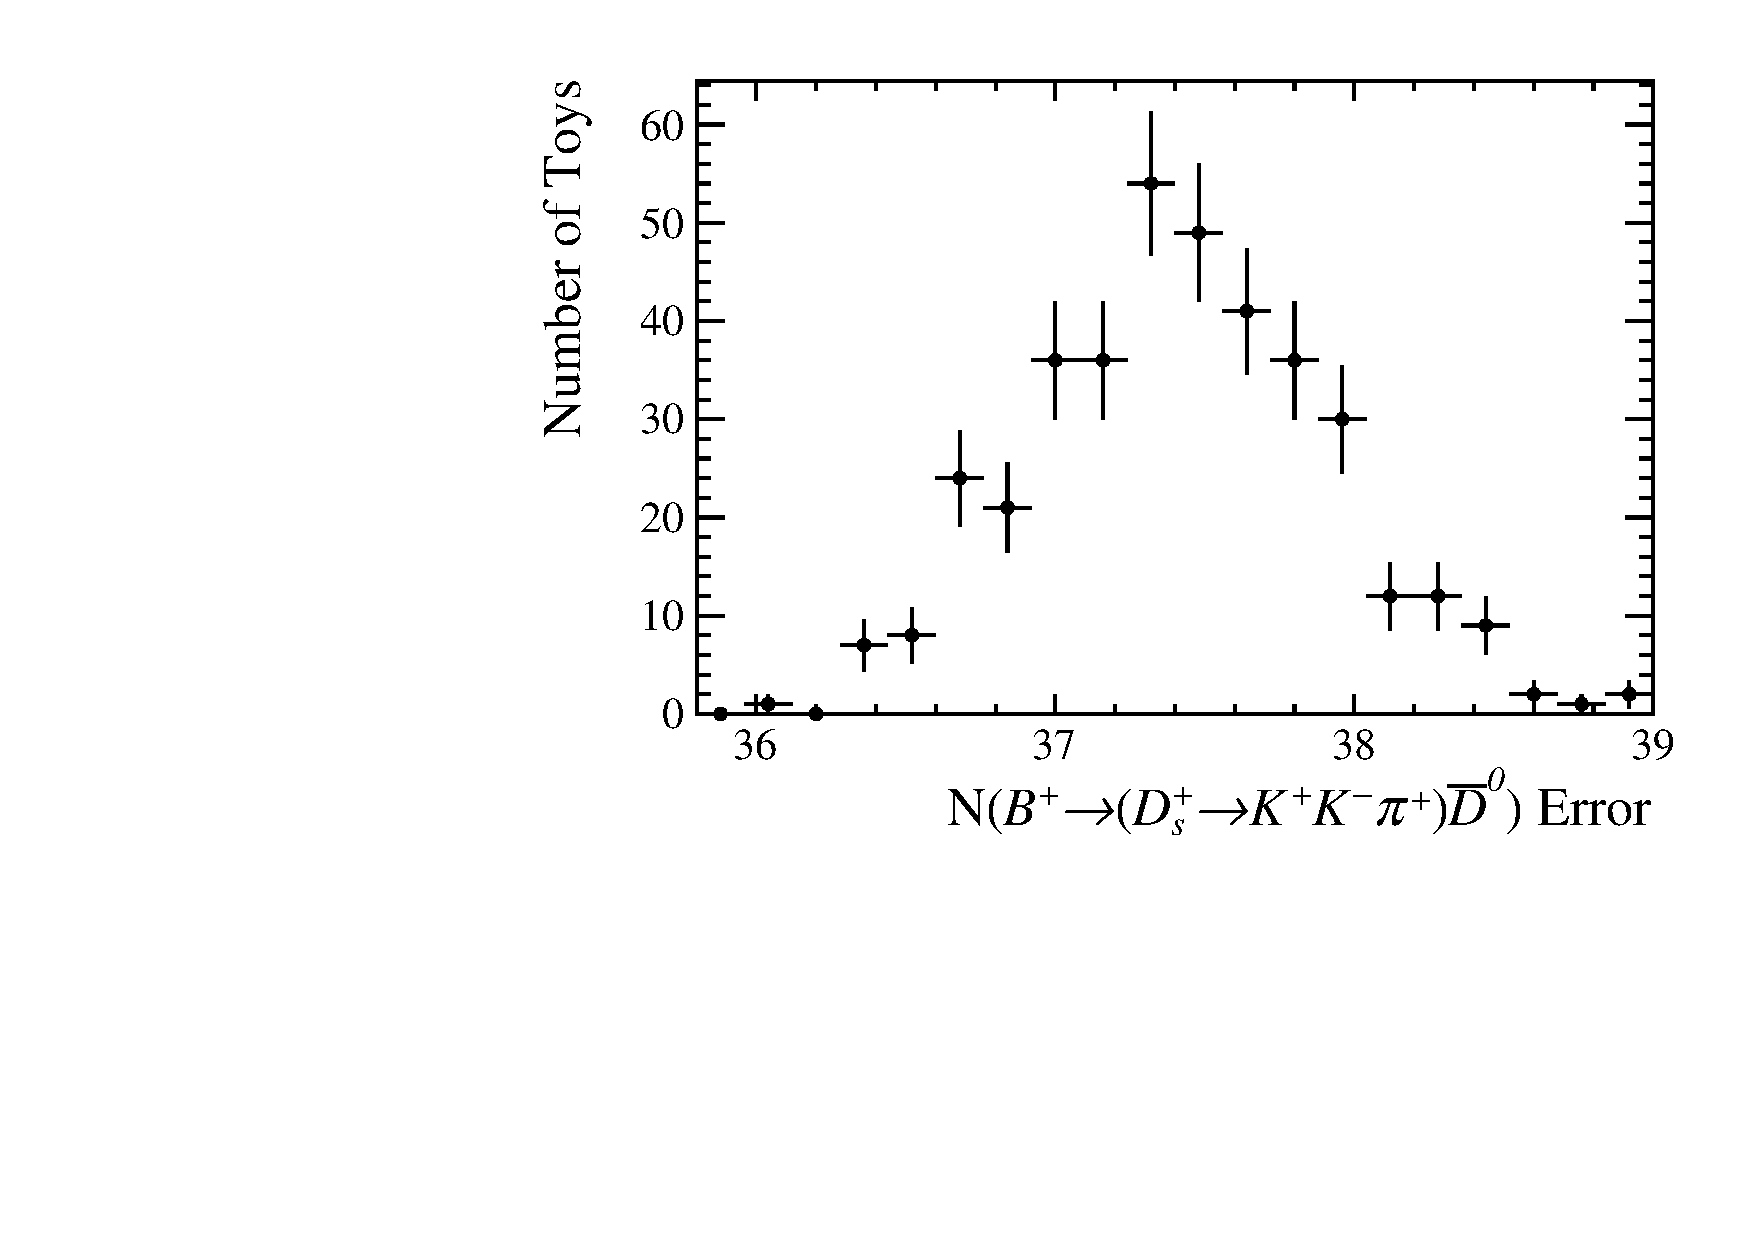
\includegraphics[width=0.32\textwidth]{figs/B2DsPhi/Plots_DsKK_Error_yield_peak_DsD0_Ds2KKPi_toy_both_DsBDTbin1_PhiBDTbin1_both_both.pdf}
      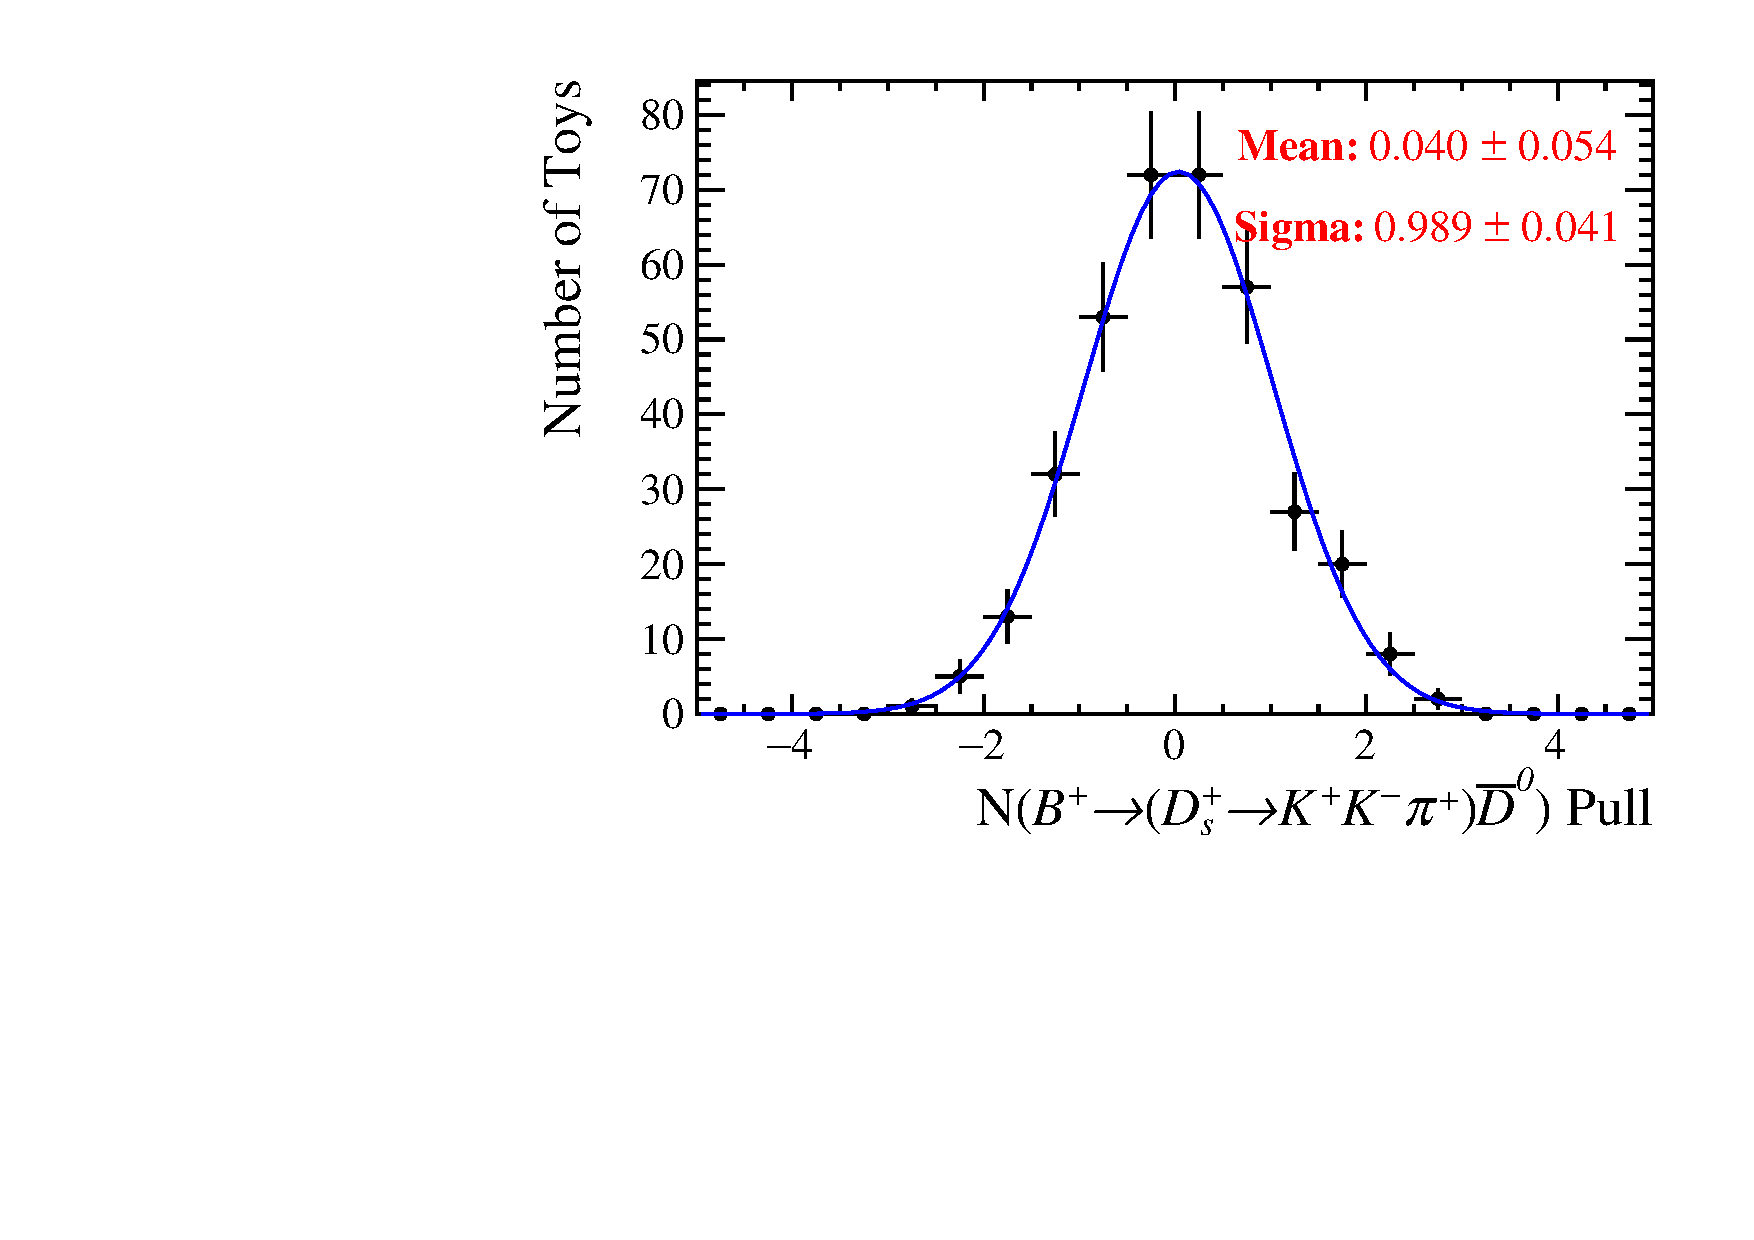
\includegraphics[width=0.32\textwidth]{figs/B2DsPhi/Plots_DsKK_Pull_yield_peak_DsD0_Ds2KKPi_toy_both_DsBDTbin1_PhiBDTbin1_both_both.pdf}
      \caption{\decay{\Dsp}{\Kp\Km\pip}}
   \end{subfigure}\\
   \begin{subfigure}[t]{1.0\textwidth}
      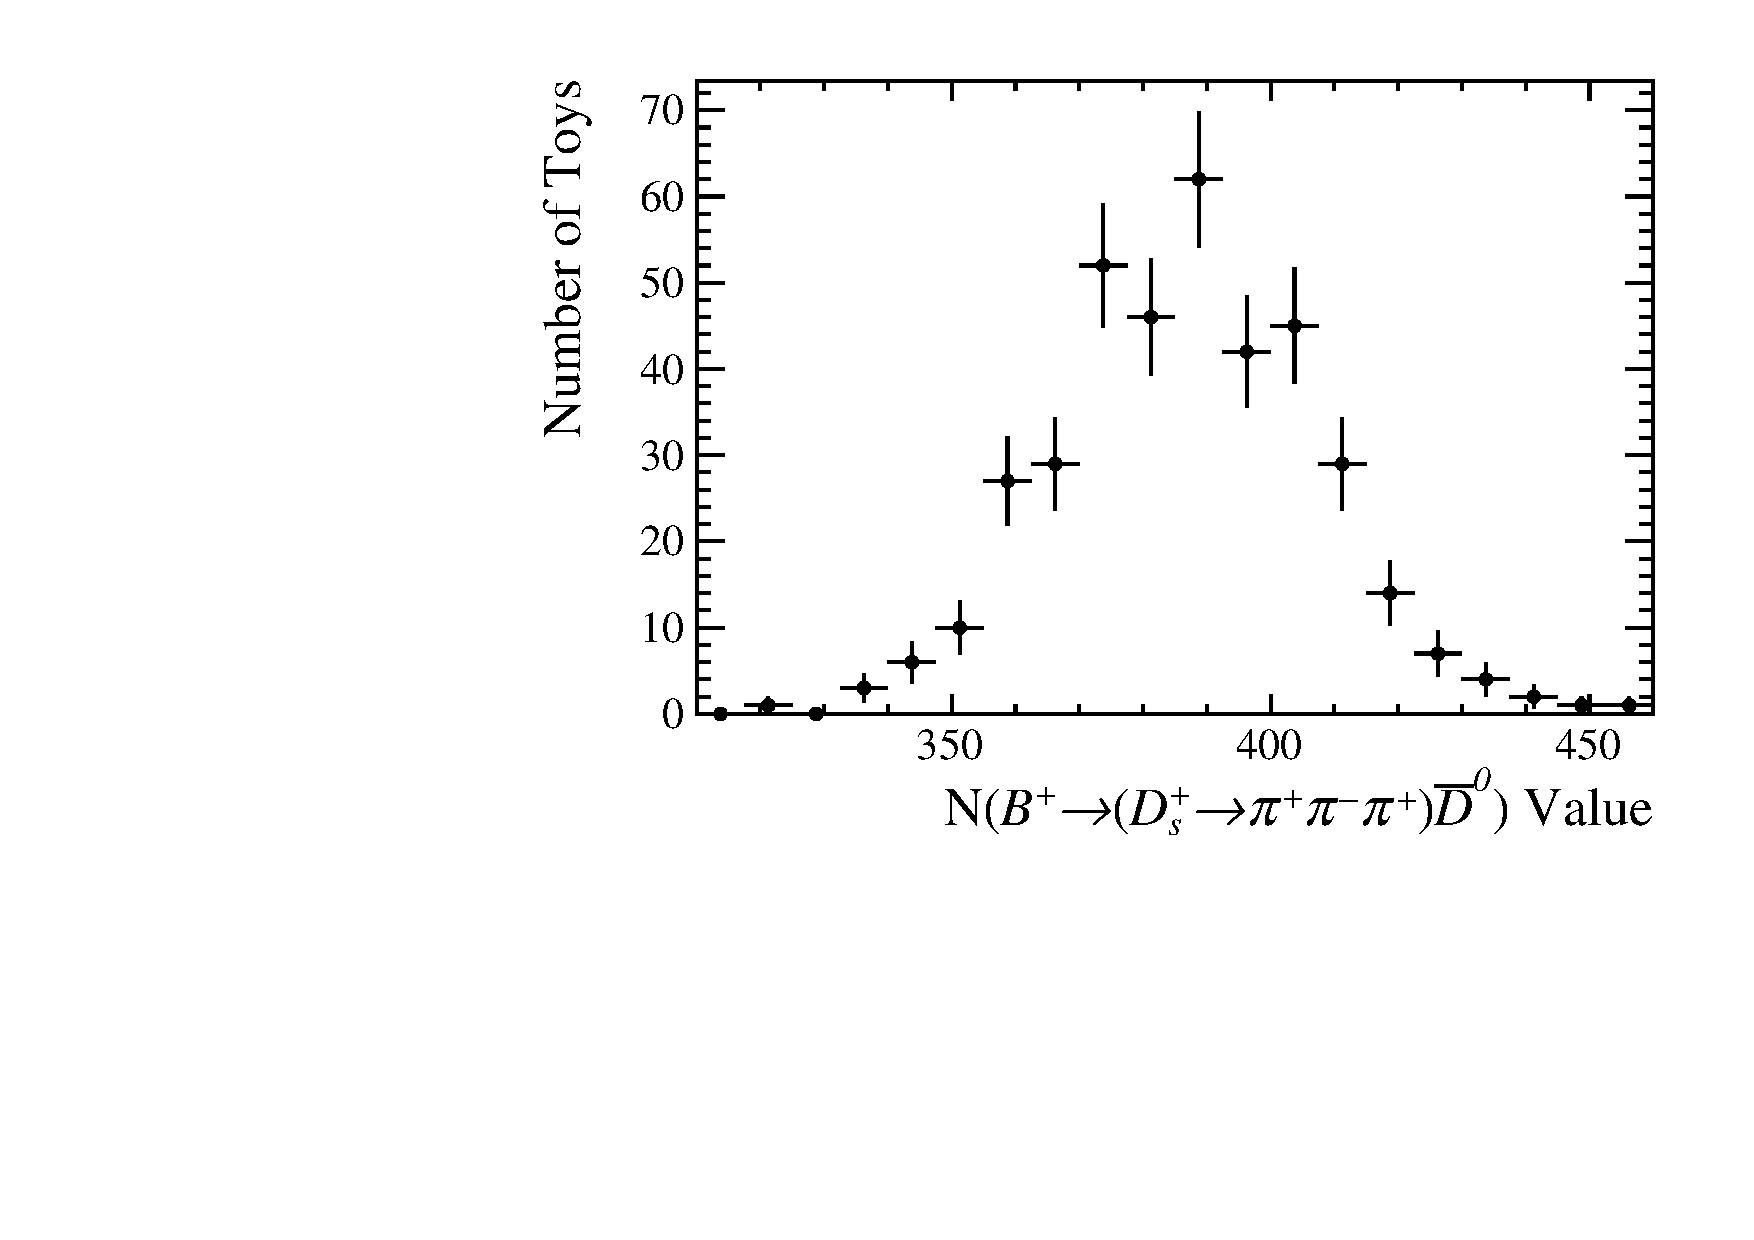
\includegraphics[width=0.32\textwidth]{figs/B2DsPhi/Plots_DsKK_Value_yield_peak_DsD0_Ds2PiPiPi_toy_both_DsBDTbin1_PhiBDTbin1_both_both.pdf}
      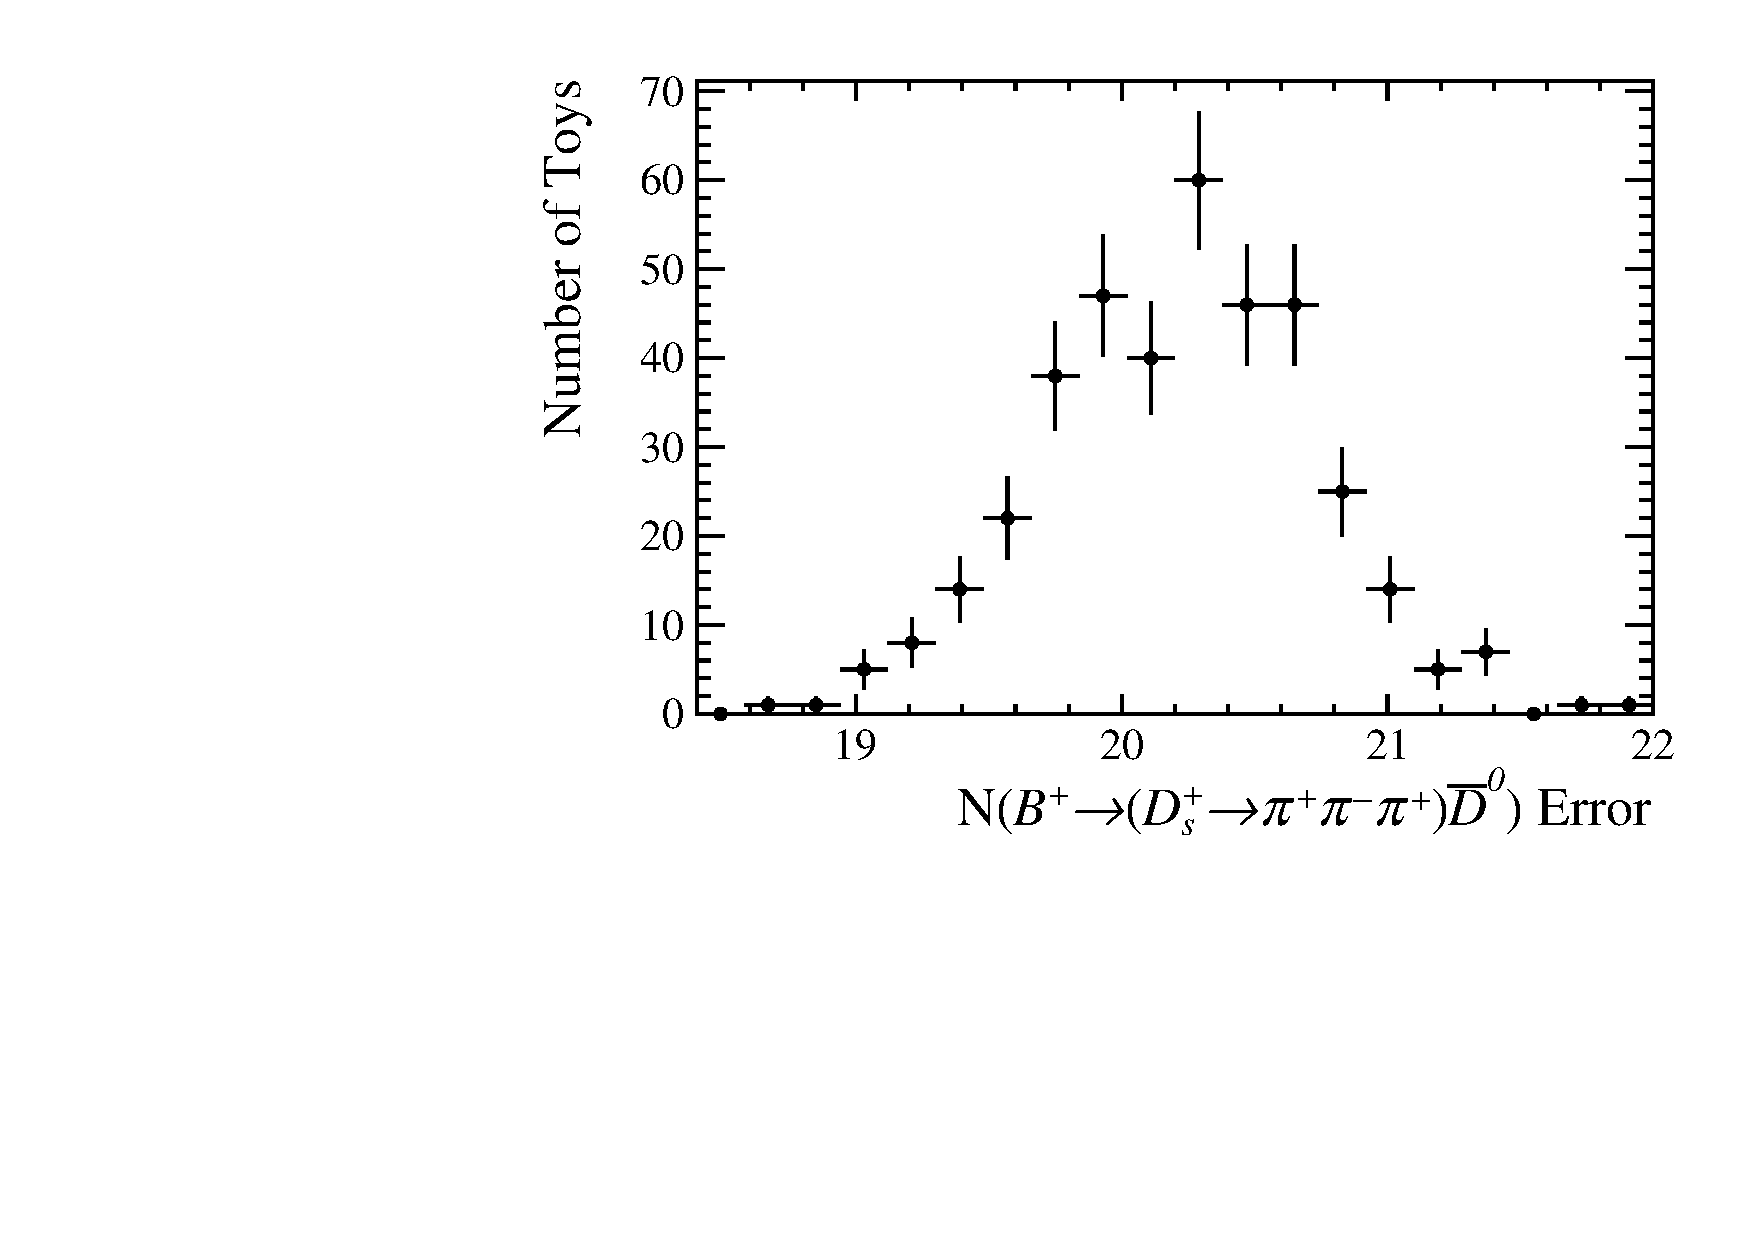
\includegraphics[width=0.32\textwidth]{figs/B2DsPhi/Plots_DsKK_Error_yield_peak_DsD0_Ds2PiPiPi_toy_both_DsBDTbin1_PhiBDTbin1_both_both.pdf}
      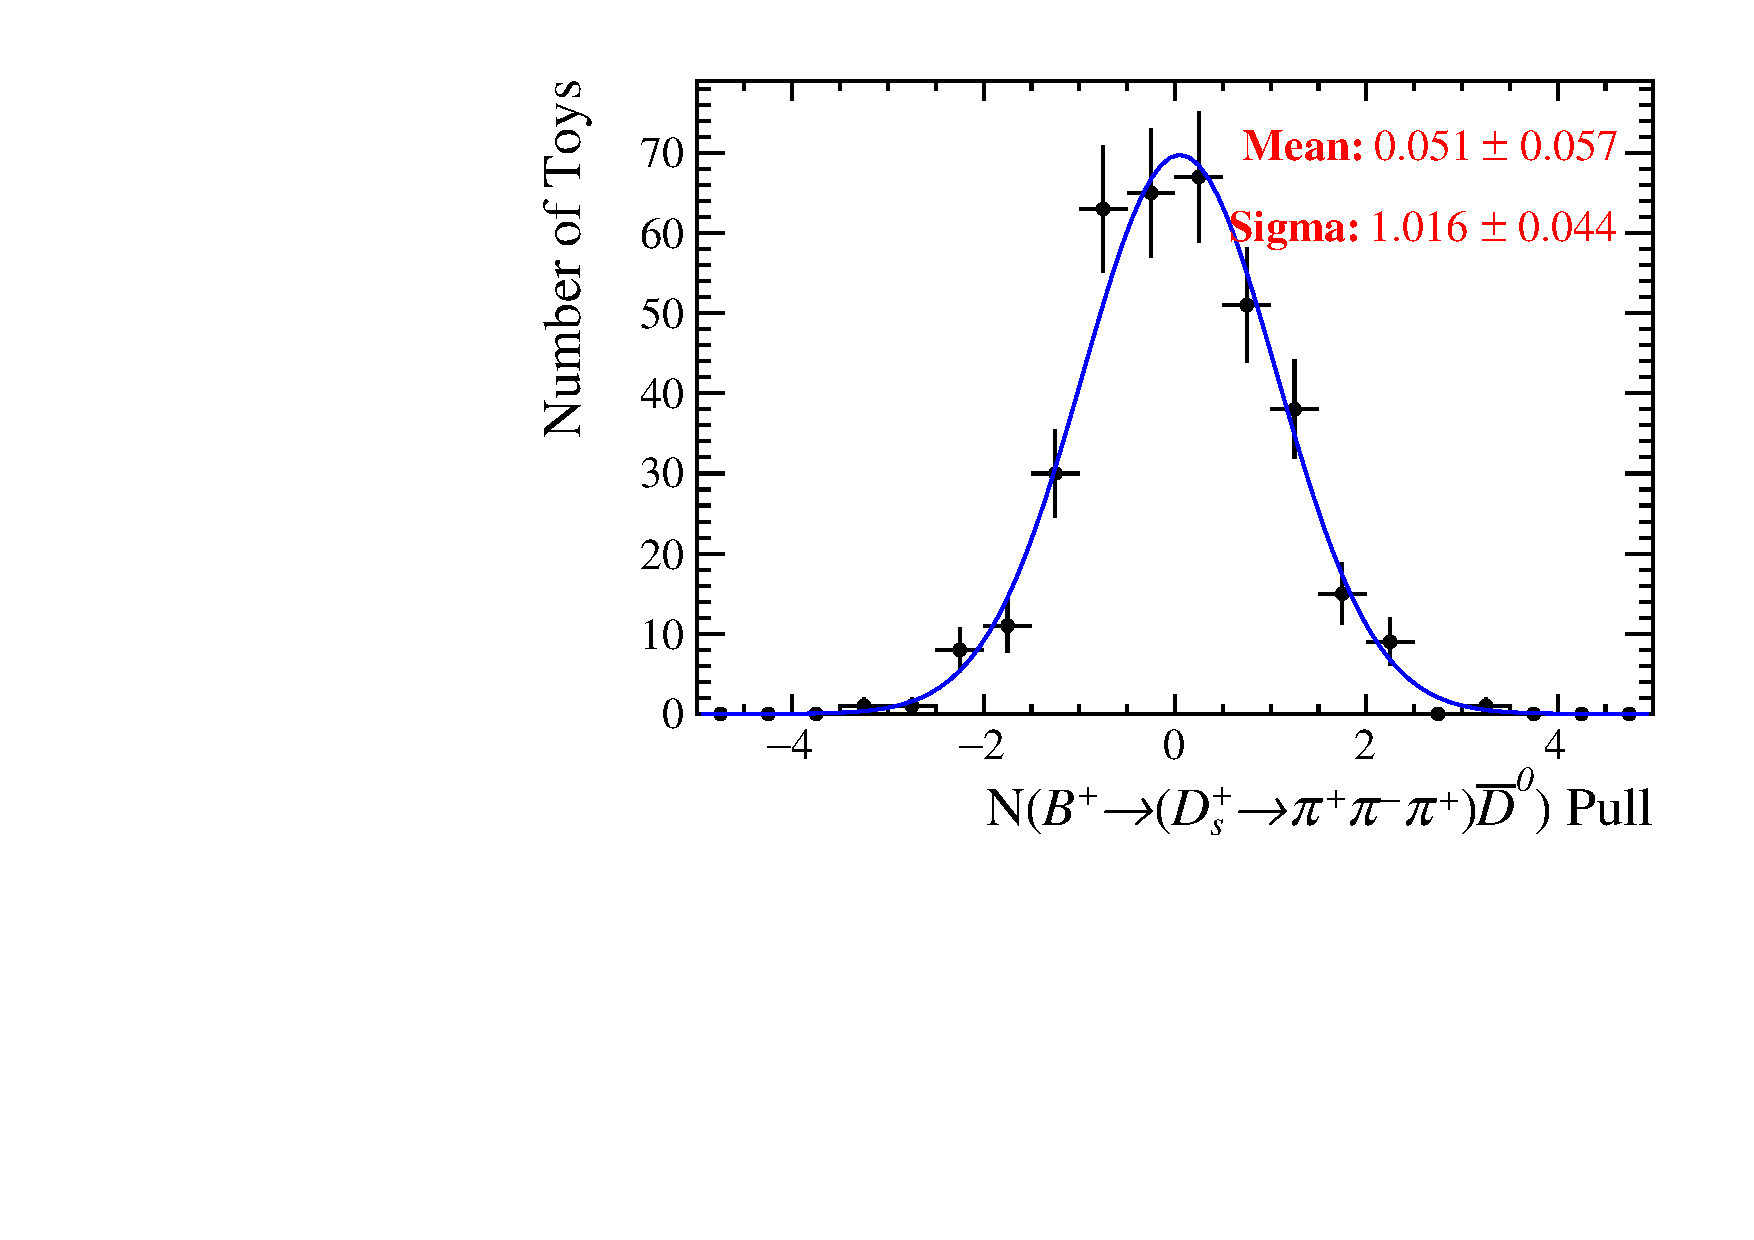
\includegraphics[width=0.32\textwidth]{figs/B2DsPhi/Plots_DsKK_Pull_yield_peak_DsD0_Ds2PiPiPi_toy_both_DsBDTbin1_PhiBDTbin1_both_both.pdf}
      \caption{\decay{\Dsp}{\pip\pim\pip}}
   \end{subfigure}\\
   \begin{subfigure}[t]{1.0\textwidth}
      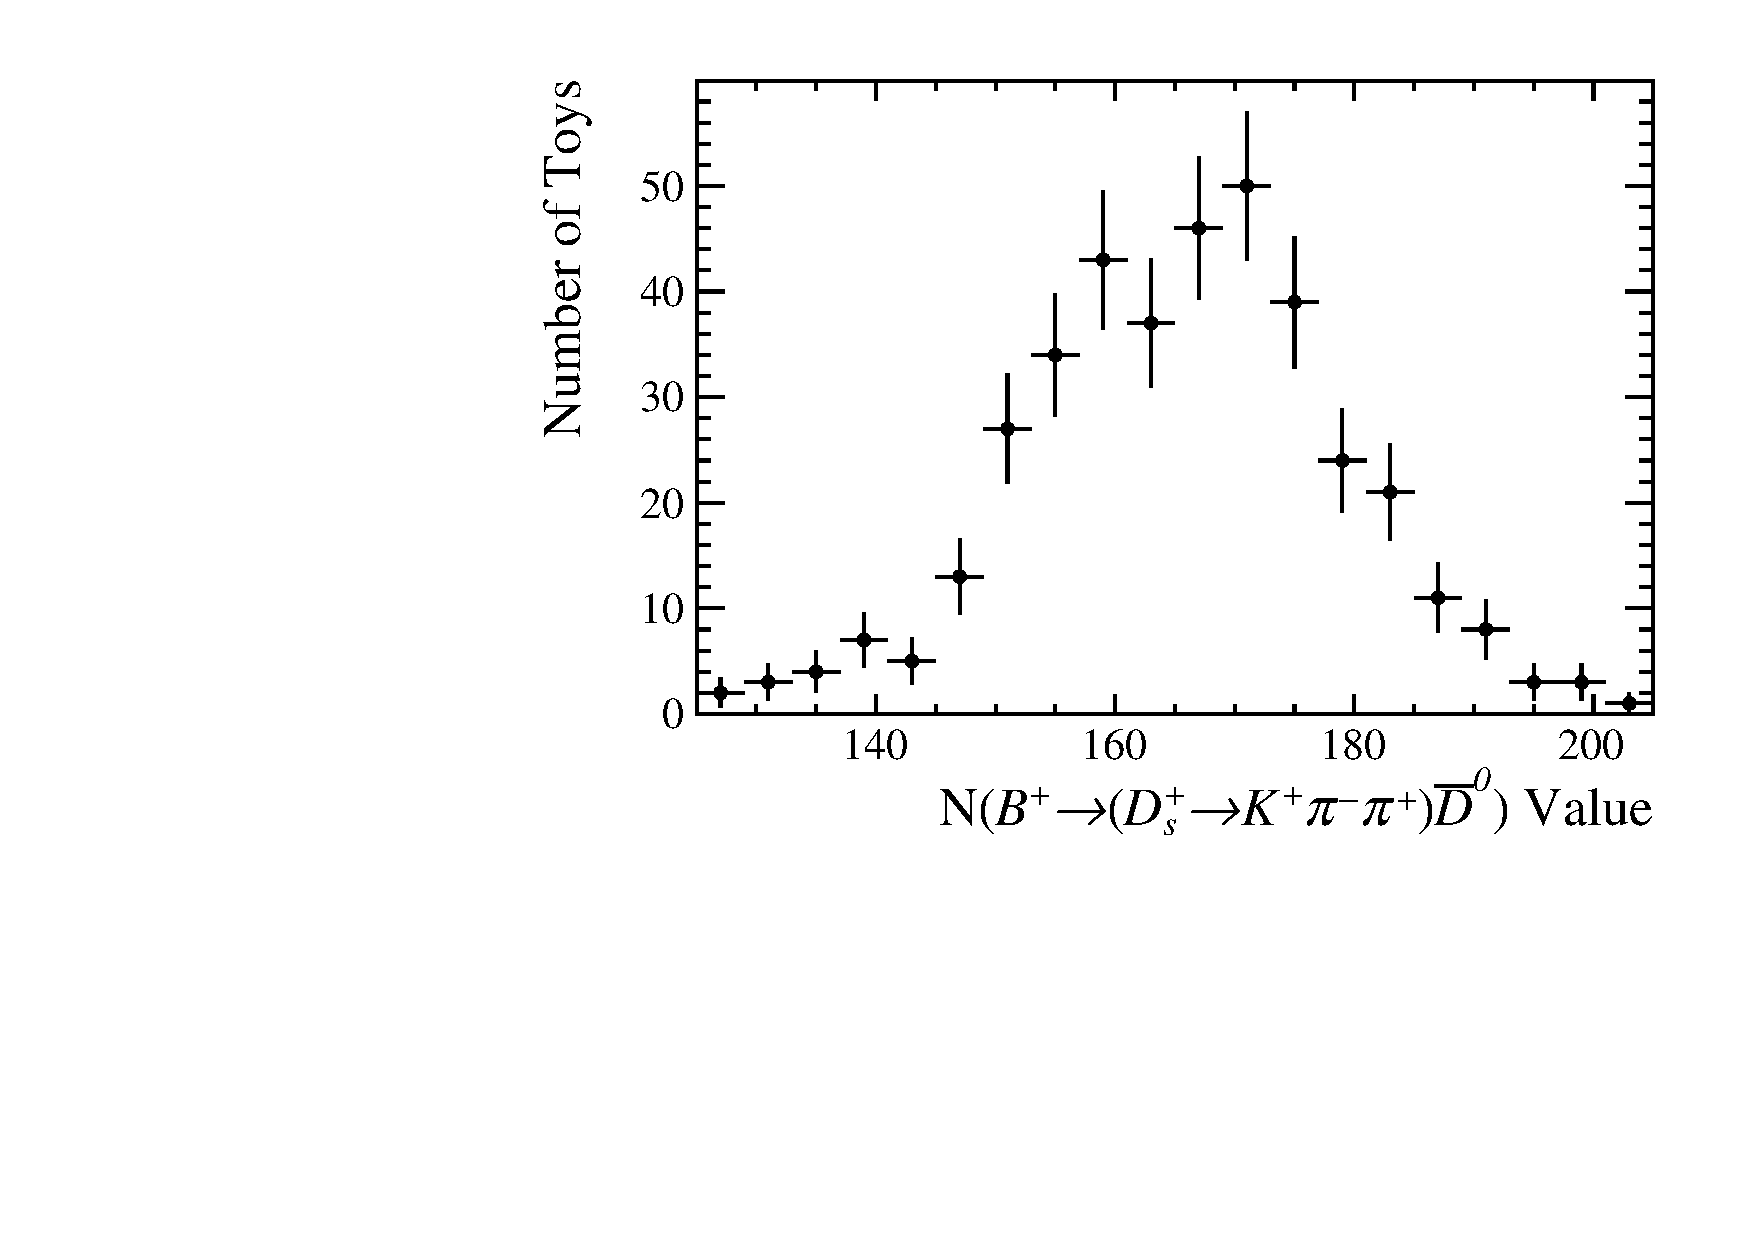
\includegraphics[width=0.32\textwidth]{figs/B2DsPhi/Plots_DsKK_Value_yield_peak_DsD0_Ds2KPiPi_toy_both_DsBDTbin1_PhiBDTbin1_both_both.pdf}
      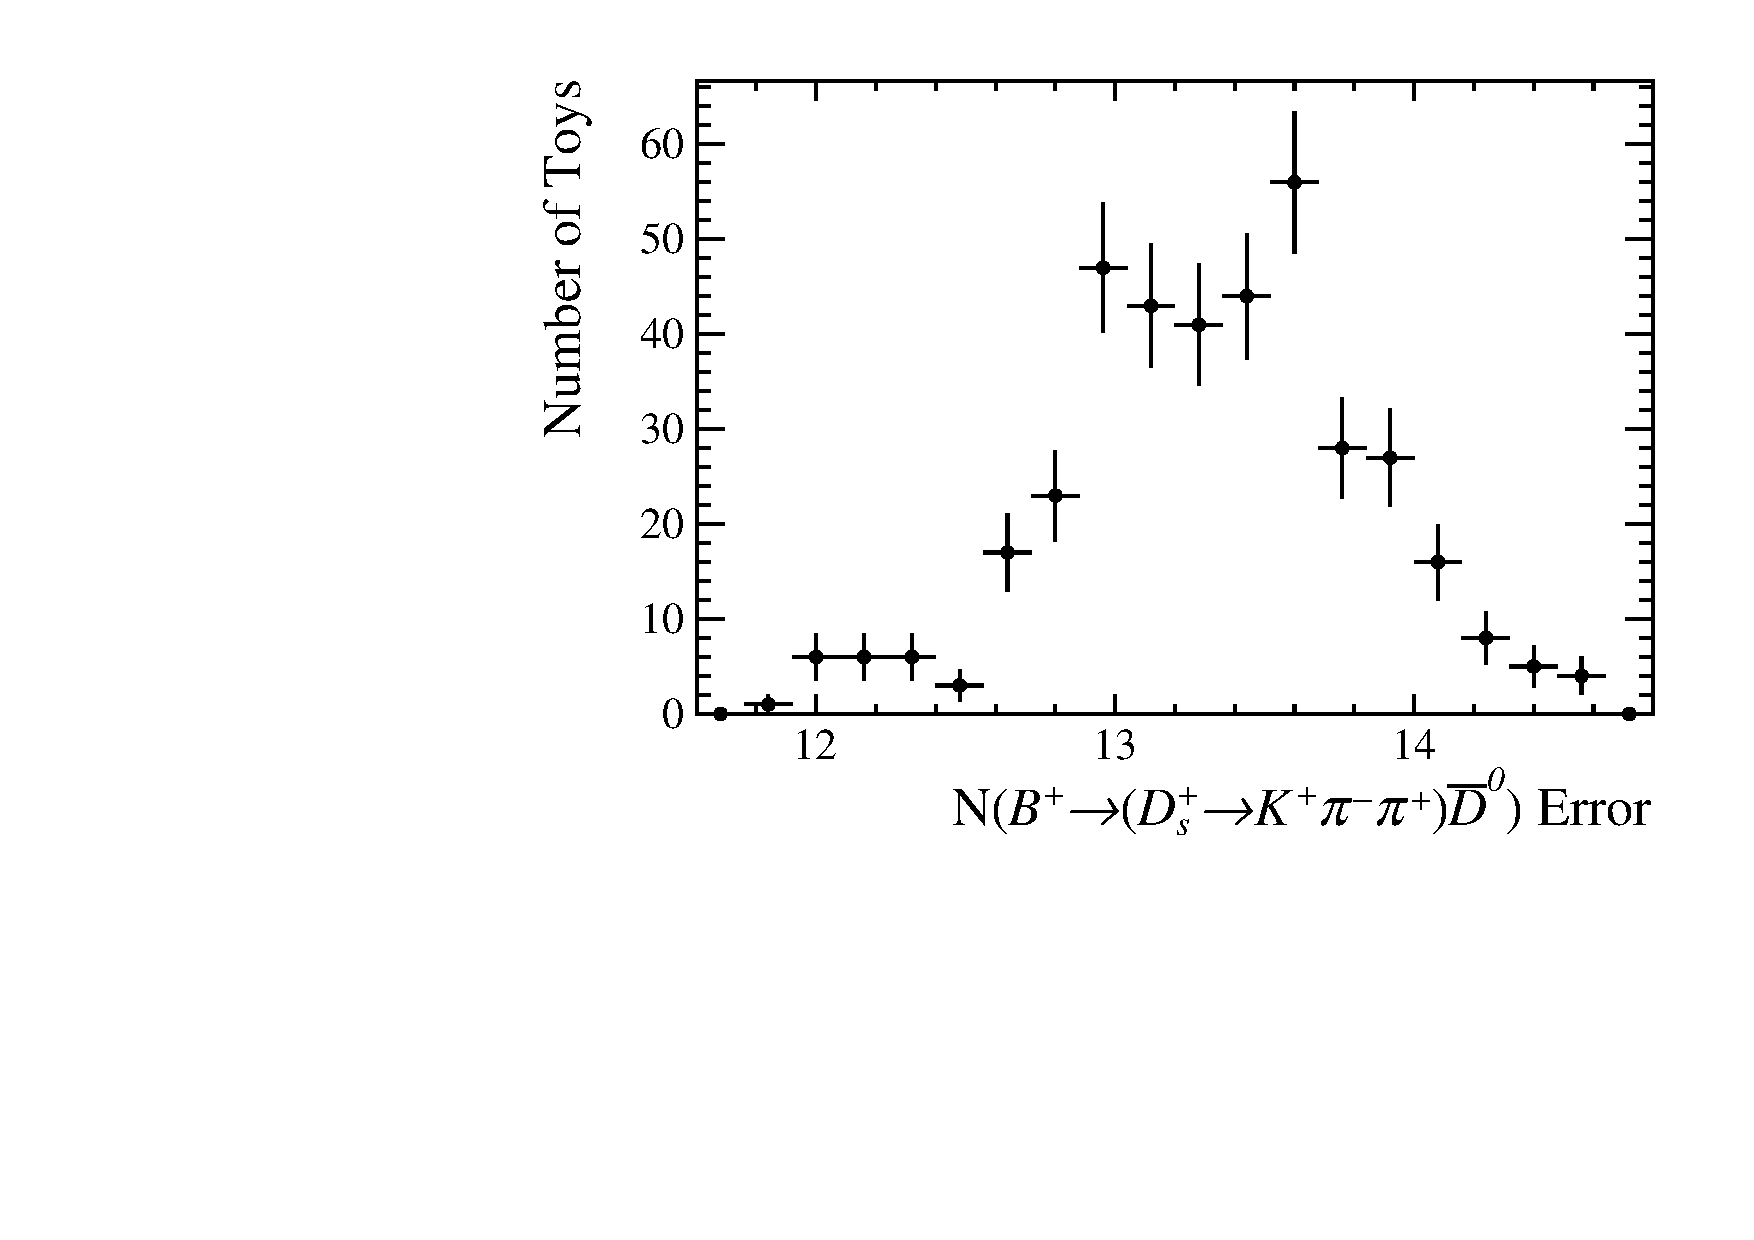
\includegraphics[width=0.32\textwidth]{figs/B2DsPhi/Plots_DsKK_Error_yield_peak_DsD0_Ds2KPiPi_toy_both_DsBDTbin1_PhiBDTbin1_both_both.pdf}
      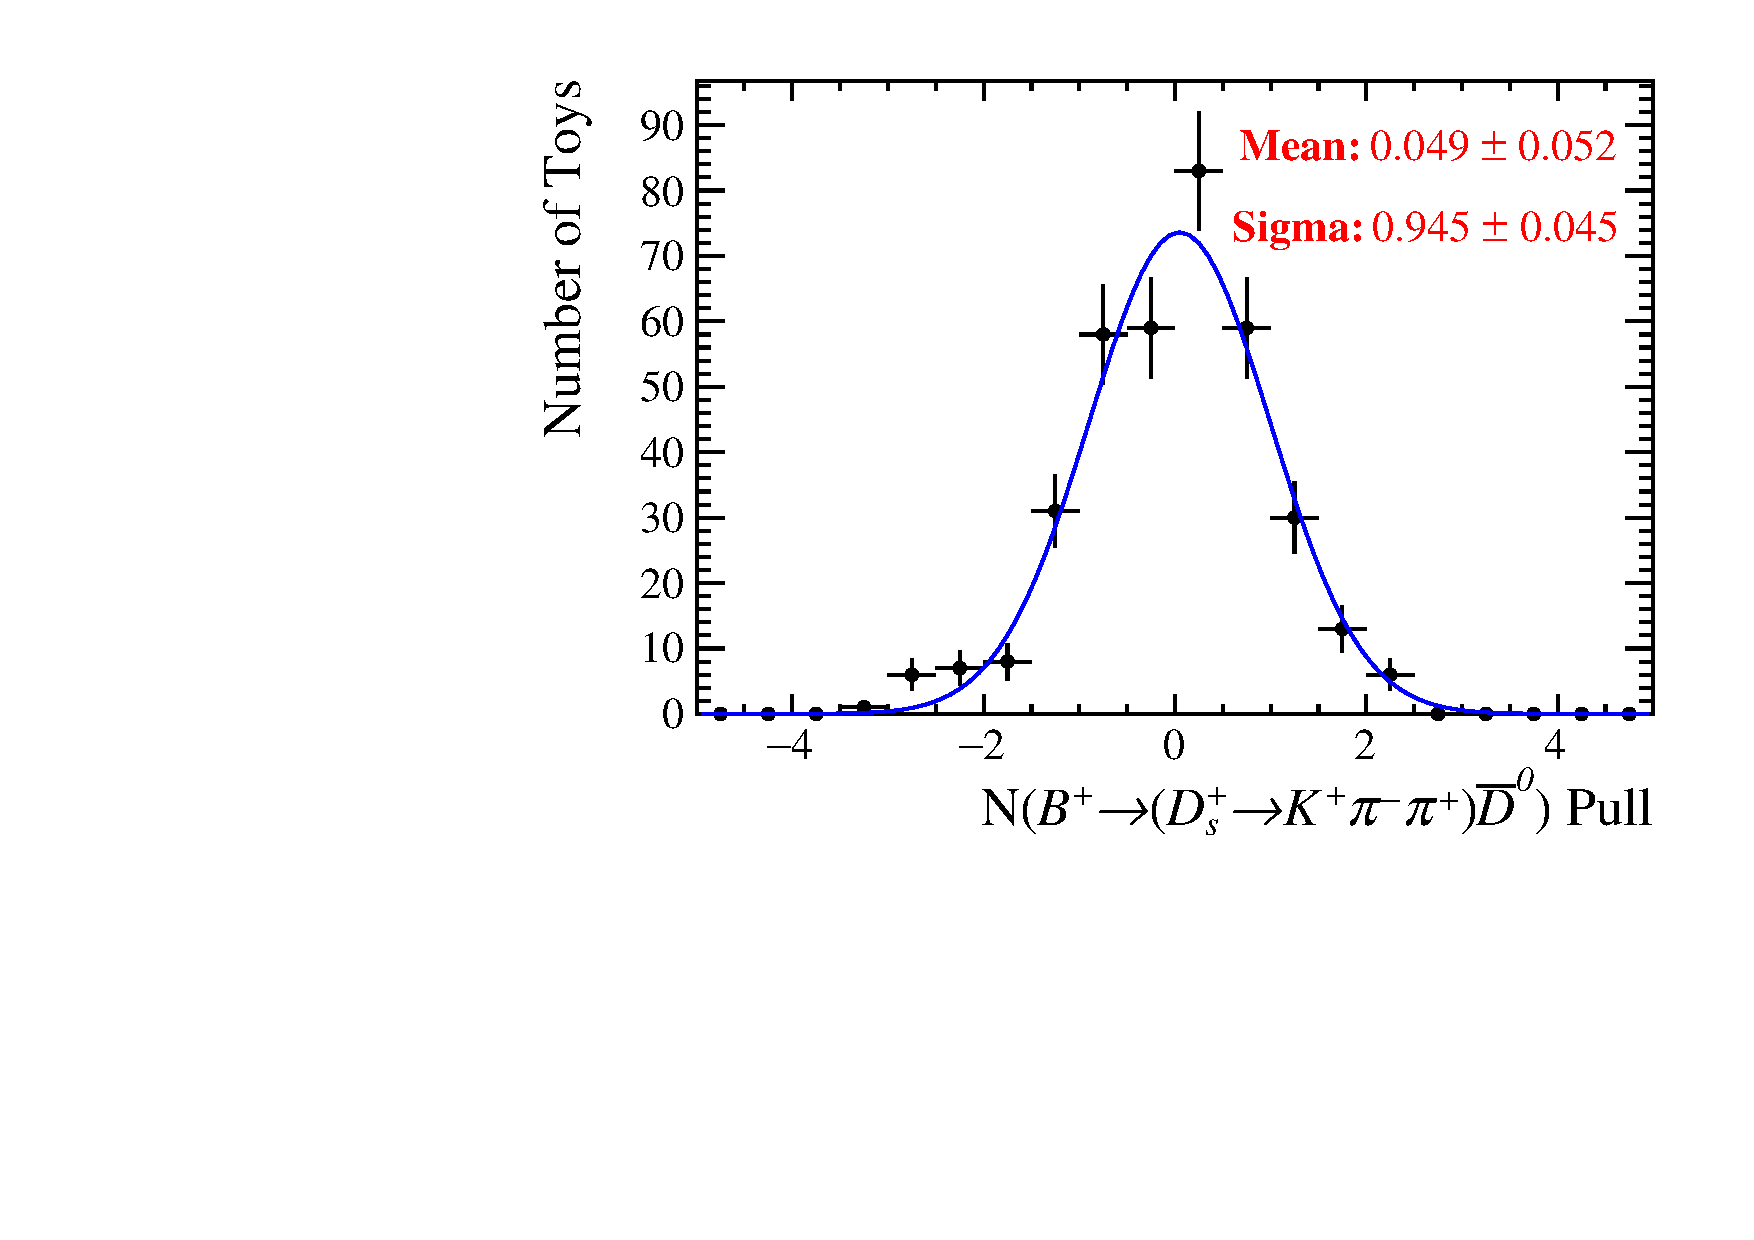
\includegraphics[width=0.32\textwidth]{figs/B2DsPhi/Plots_DsKK_Pull_yield_peak_DsD0_Ds2KPiPi_toy_both_DsBDTbin1_PhiBDTbin1_both_both.pdf}
      \caption{\decay{\Dsp}{\Kp\pim\pip}}
   \end{subfigure}

   \caption{The yield, error and pull distributions for the normalisation channel.}
   \label{fig:B2DsPhi_Pulls_normalisation}
\end{figure}
%%%%%%%%%%%%%%%%%%%%%%%%%%%%%%%%%%%%%%%%%%%%%%%%%%%%%%%%%%


Similarly, the distributions of the signal yield, error and pull for each of the different \Dsp decay modes are shown in Fig.~\ref{fig:B2DsPhi_Pulls_signal}. The pull means and widths are all within $2\sigma$ of zero and one respectively.


%%%%%%%%%%%%%%%%%%%%%%%%%%%%%%%%%%%%%%%%%%%%%%%%%%%%%%%%%%
\begin{figure}[!h]
   \centering
   \begin{subfigure}[t]{1.0\textwidth}
      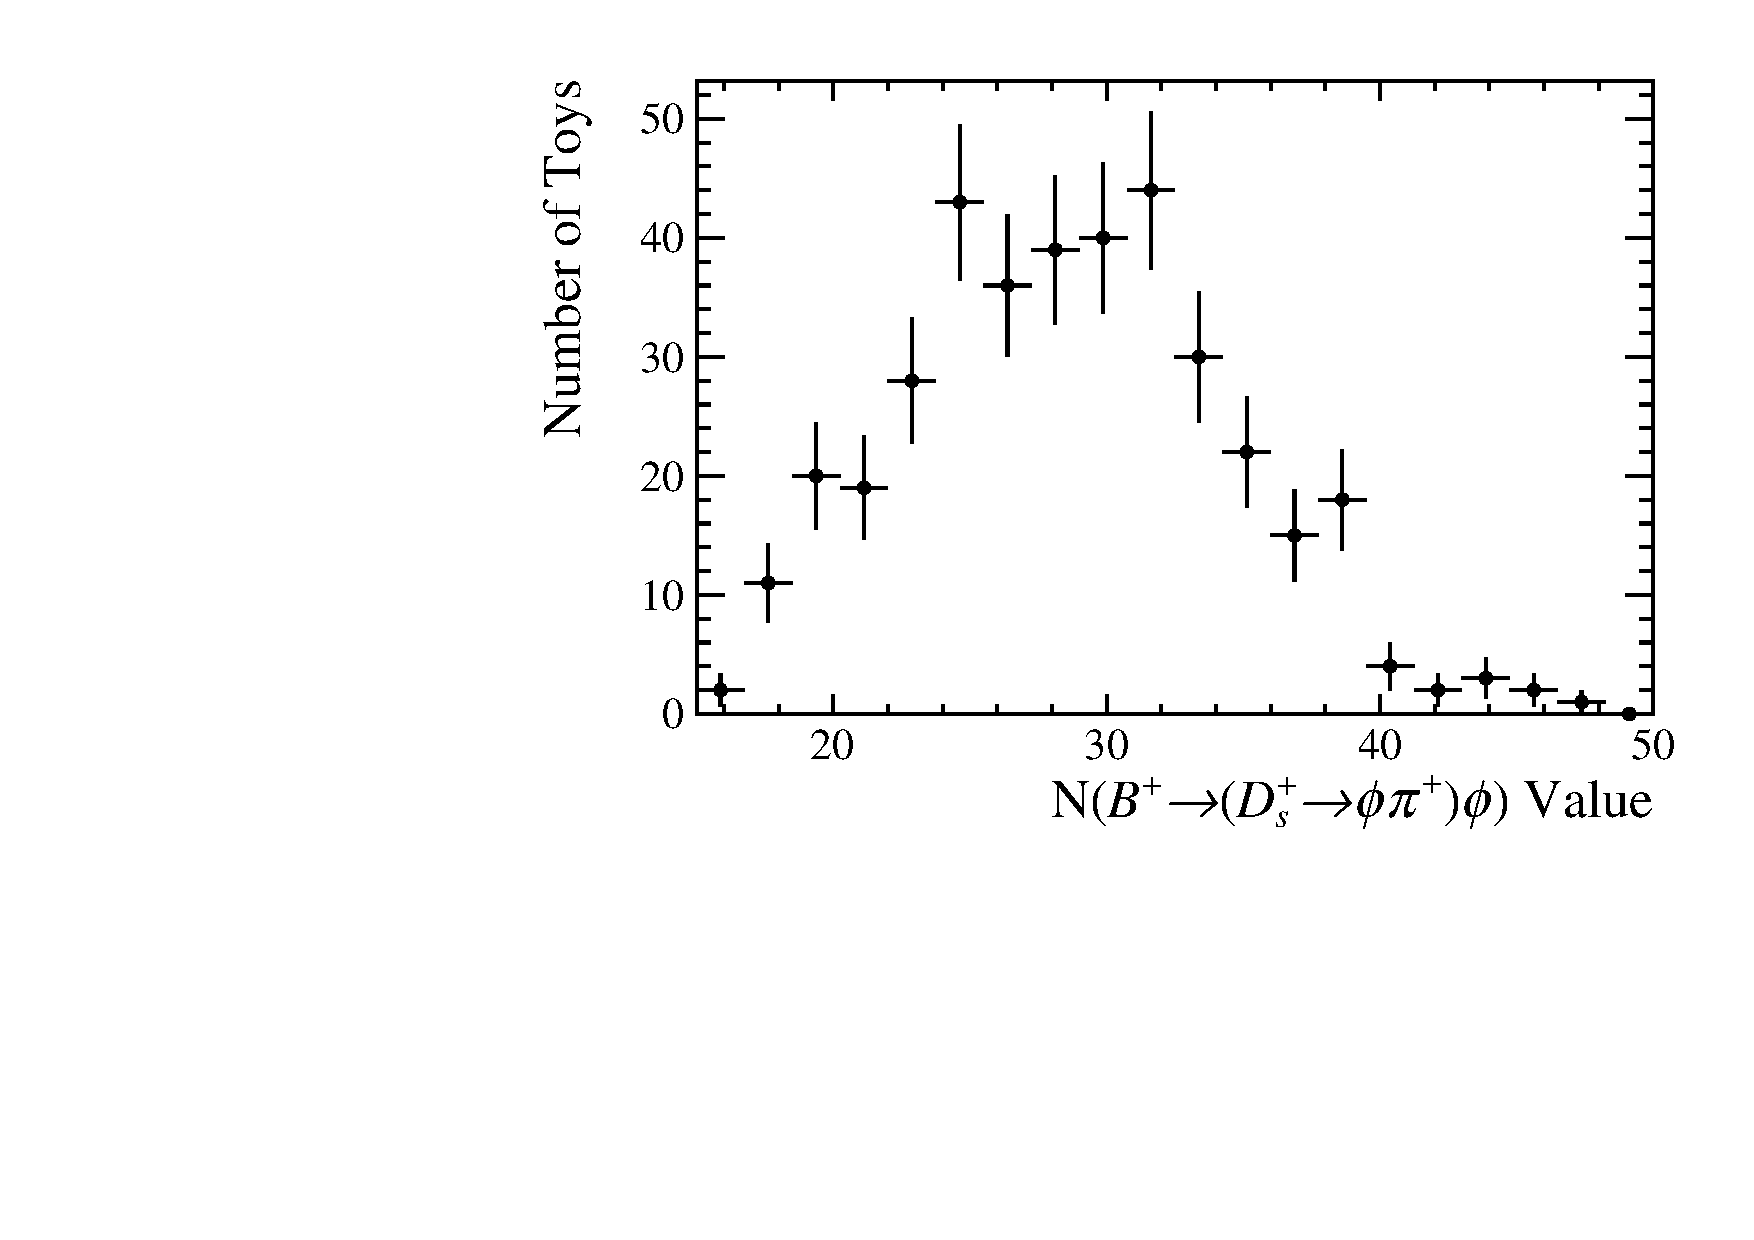
\includegraphics[width=0.32\textwidth]{figs/B2DsPhi/Plots_DsKK_Value_yield_peak_total_DsPhi_Ds2PhiPi_toy_both_DsBDTbin1_PhiBDTbin1_both_both.pdf}
      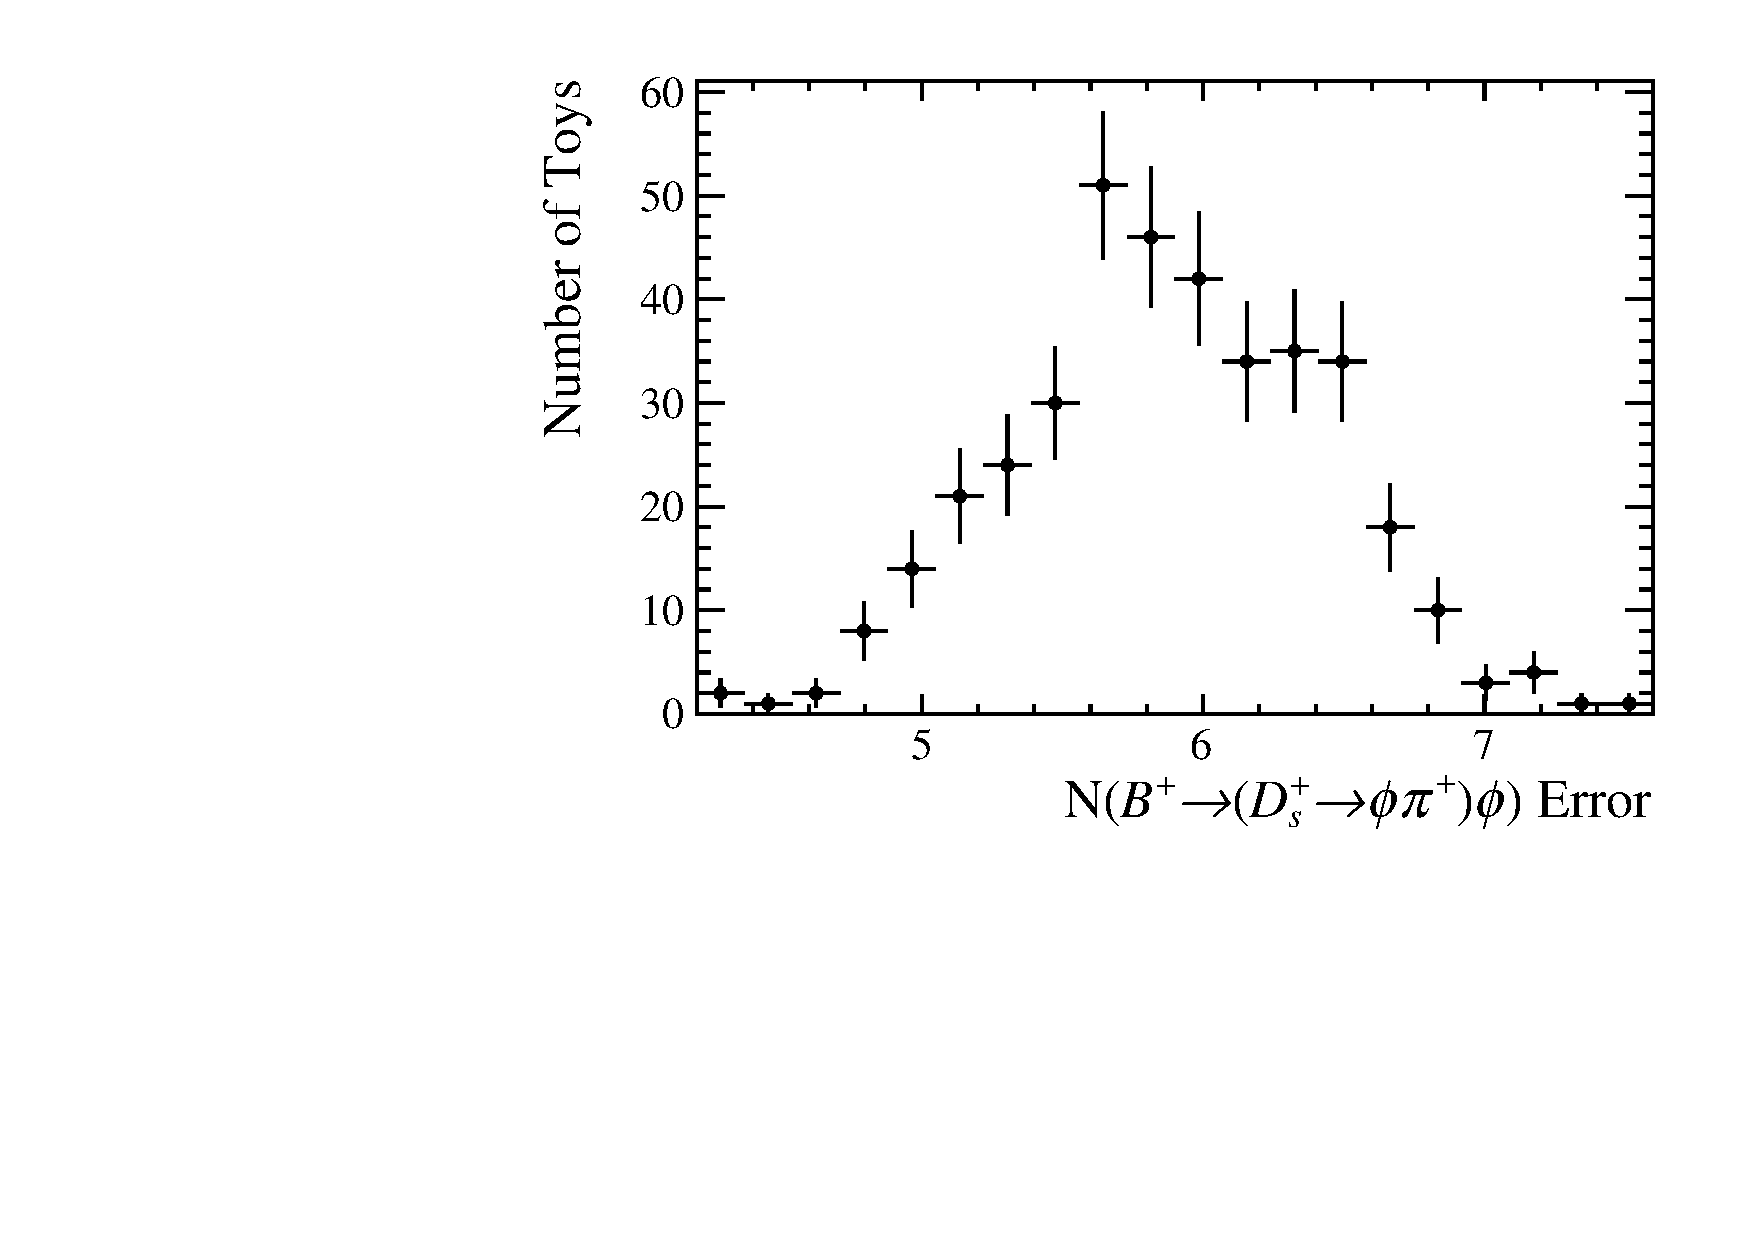
\includegraphics[width=0.32\textwidth]{figs/B2DsPhi/Plots_DsKK_Error_yield_peak_total_DsPhi_Ds2PhiPi_toy_both_DsBDTbin1_PhiBDTbin1_both_both.pdf}
      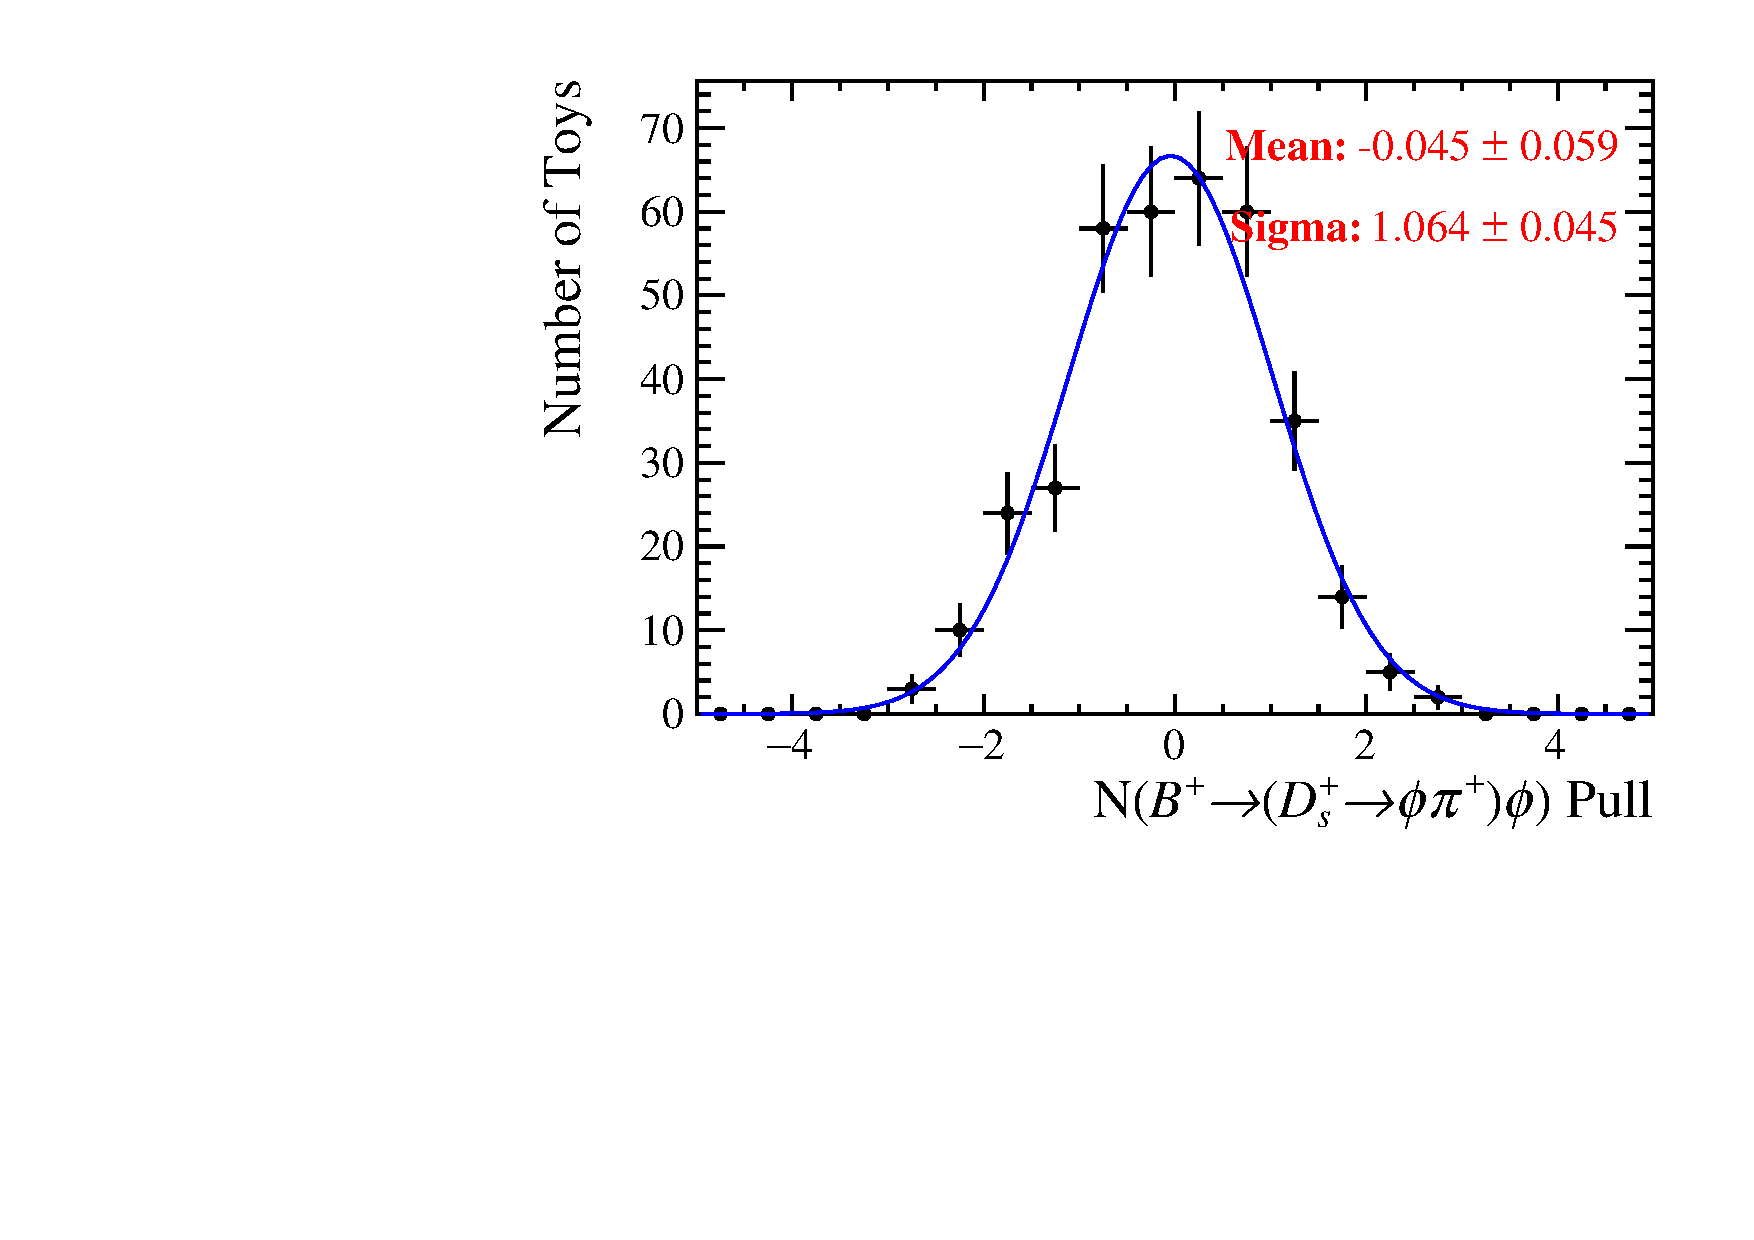
\includegraphics[width=0.32\textwidth]{figs/B2DsPhi/Plots_DsKK_Pull_yield_peak_total_DsPhi_Ds2PhiPi_toy_both_DsBDTbin1_PhiBDTbin1_both_both.pdf}
      \caption{\decay{\Dsp}{\phiz\pip}}
   \end{subfigure}\\
   \begin{subfigure}[t]{1.0\textwidth}
      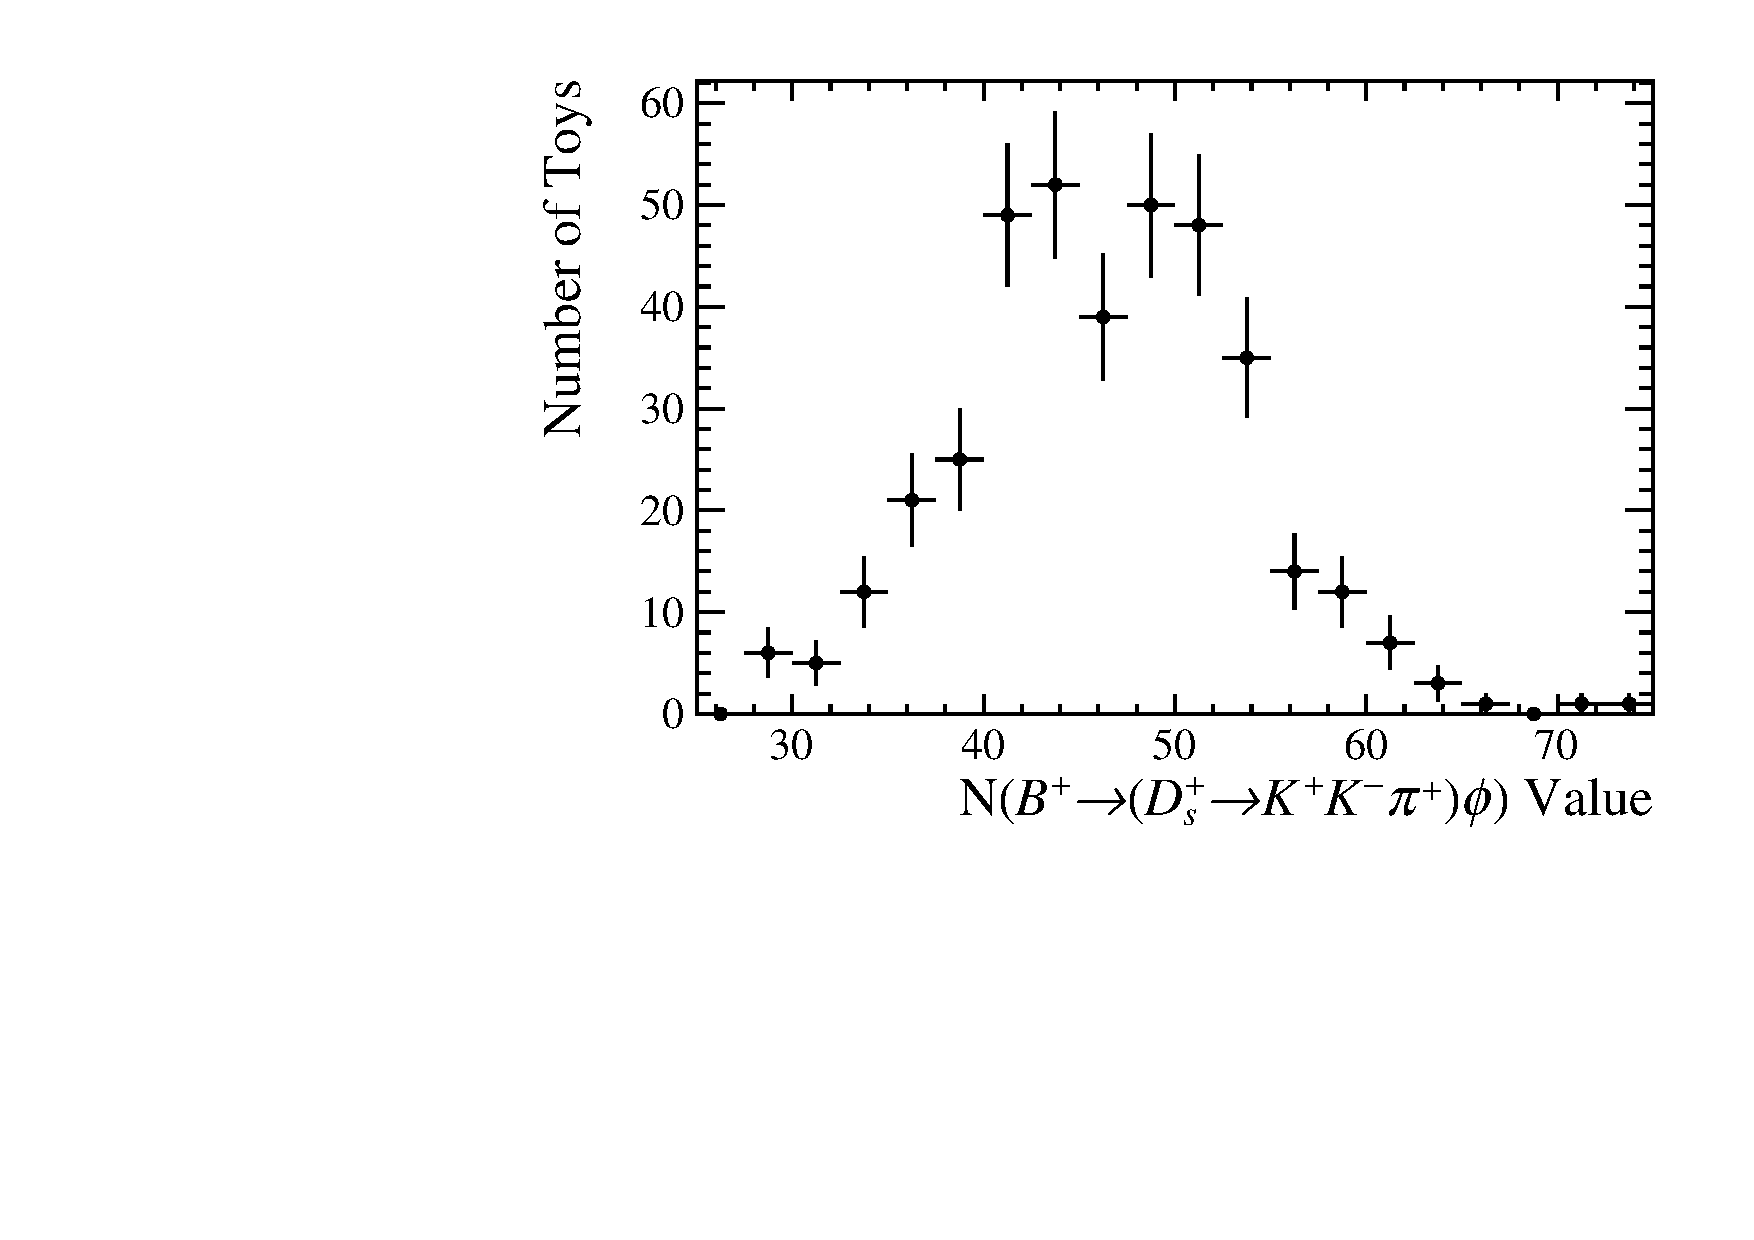
\includegraphics[width=0.32\textwidth]{figs/B2DsPhi/Plots_DsKK_Value_yield_peak_total_DsPhi_Ds2KKPi_toy_both_DsBDTbin1_PhiBDTbin1_both_both.pdf}
      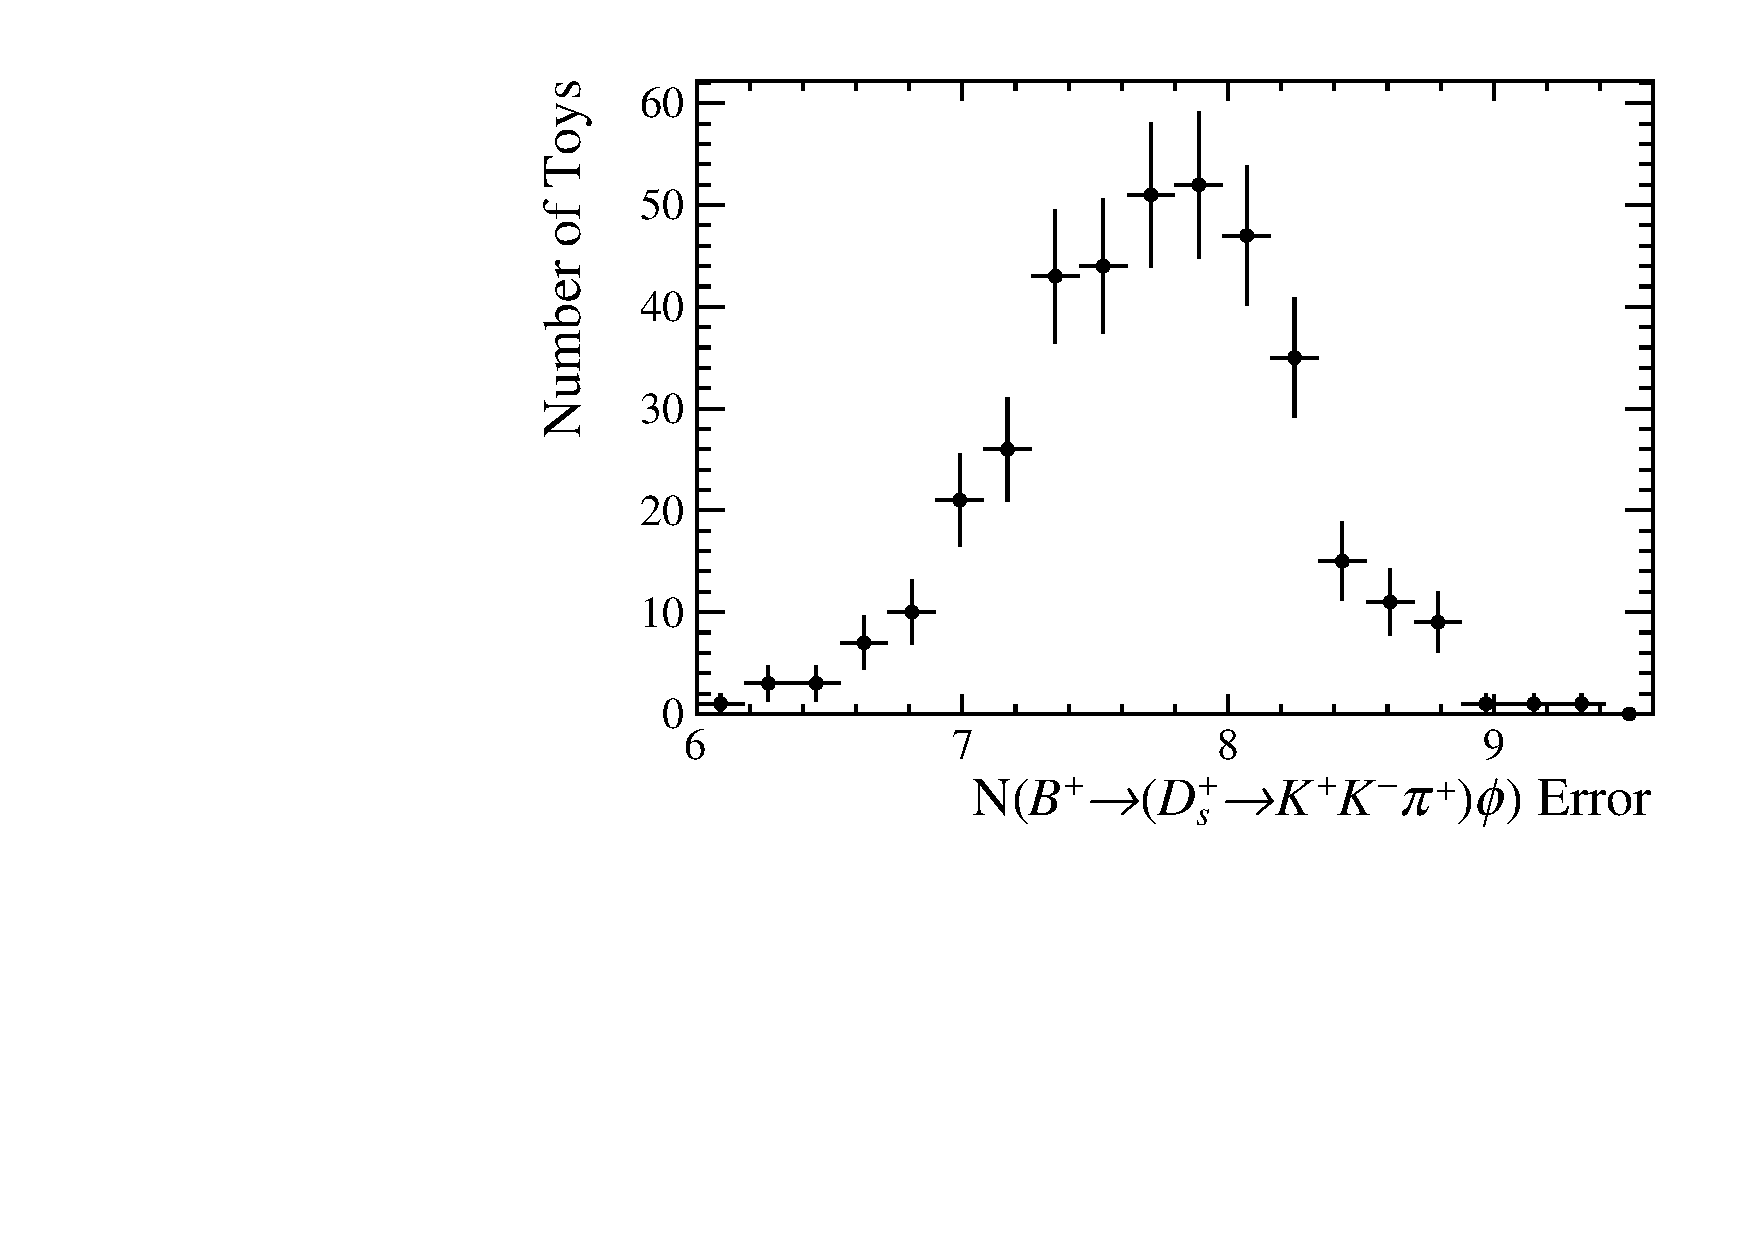
\includegraphics[width=0.32\textwidth]{figs/B2DsPhi/Plots_DsKK_Error_yield_peak_total_DsPhi_Ds2KKPi_toy_both_DsBDTbin1_PhiBDTbin1_both_both.pdf}
      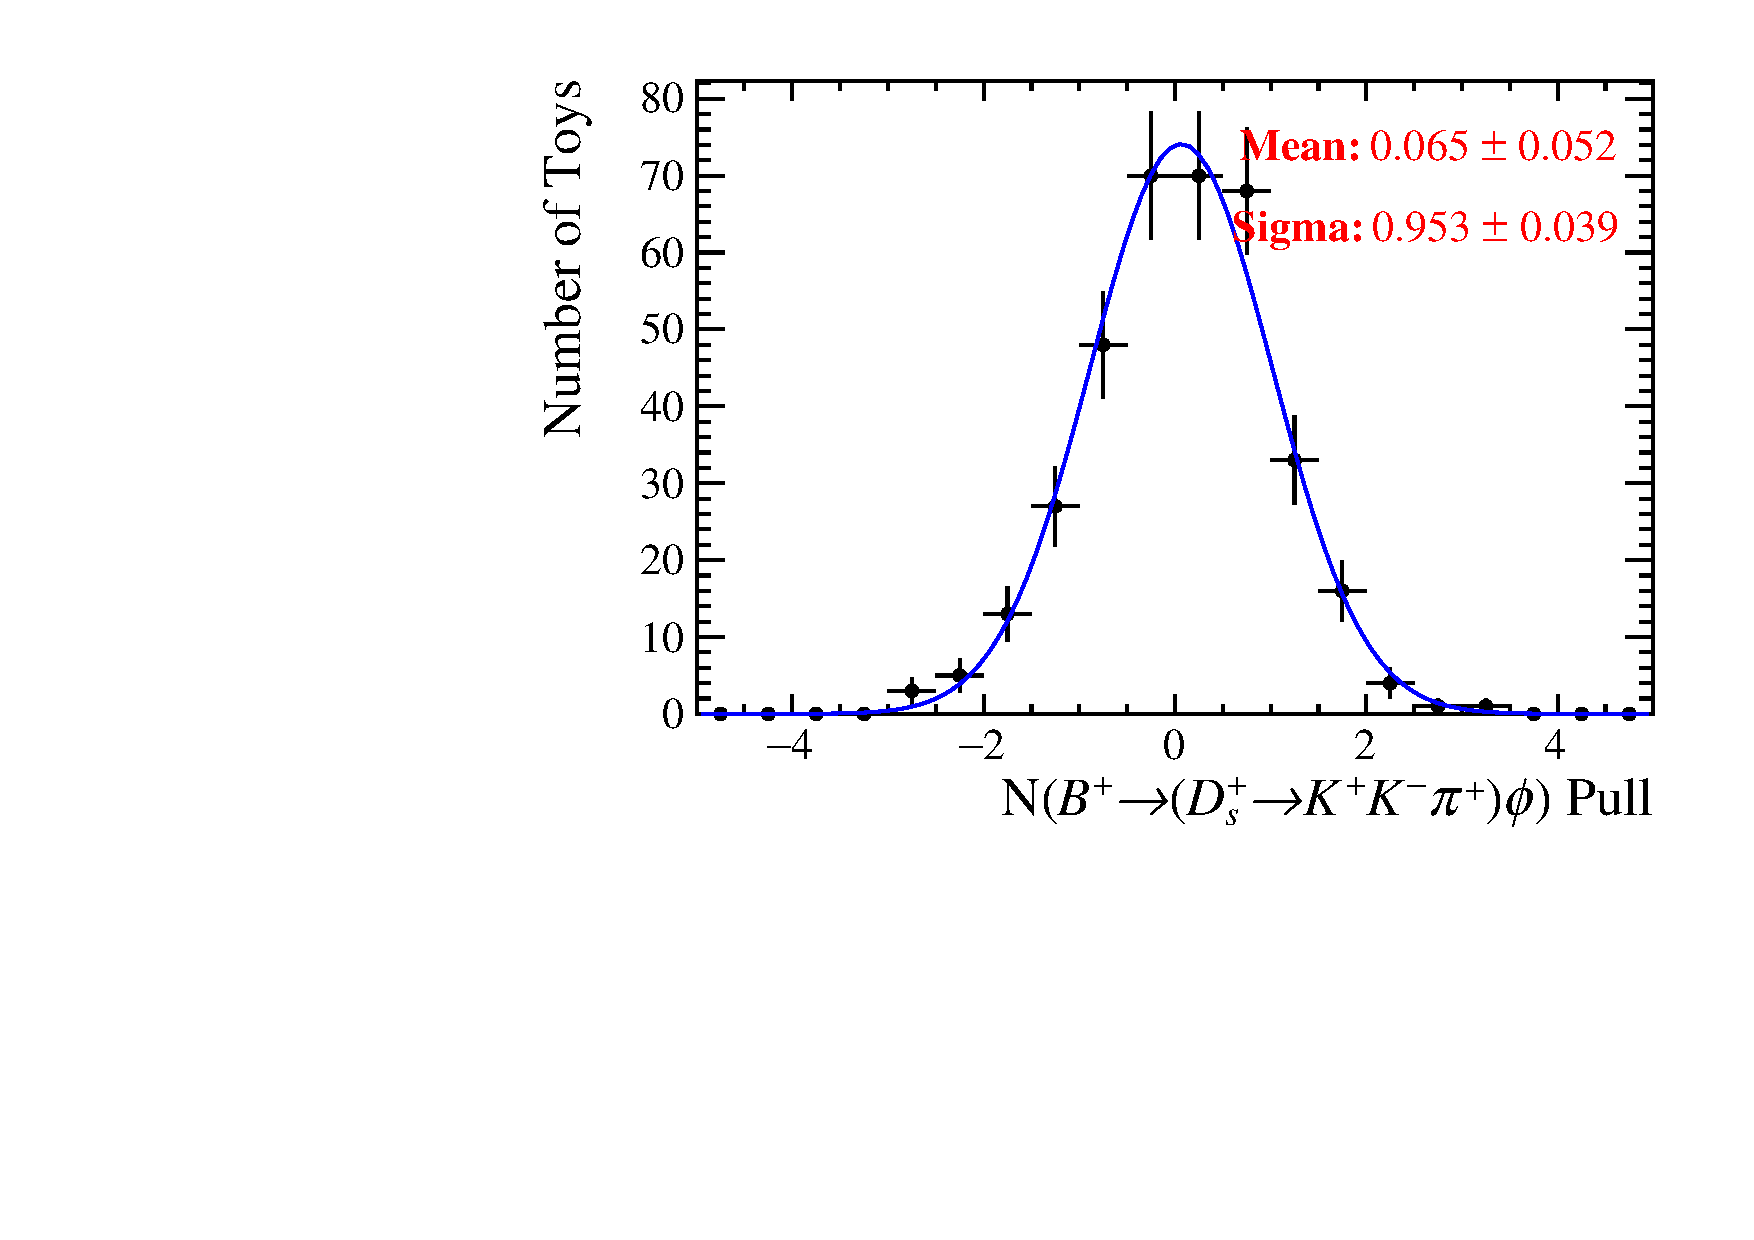
\includegraphics[width=0.32\textwidth]{figs/B2DsPhi/Plots_DsKK_Pull_yield_peak_total_DsPhi_Ds2KKPi_toy_both_DsBDTbin1_PhiBDTbin1_both_both.pdf}
      \caption{\decay{\Dsp}{\Kp\Km\pip}}
   \end{subfigure}\\
   \begin{subfigure}[t]{1.0\textwidth}
      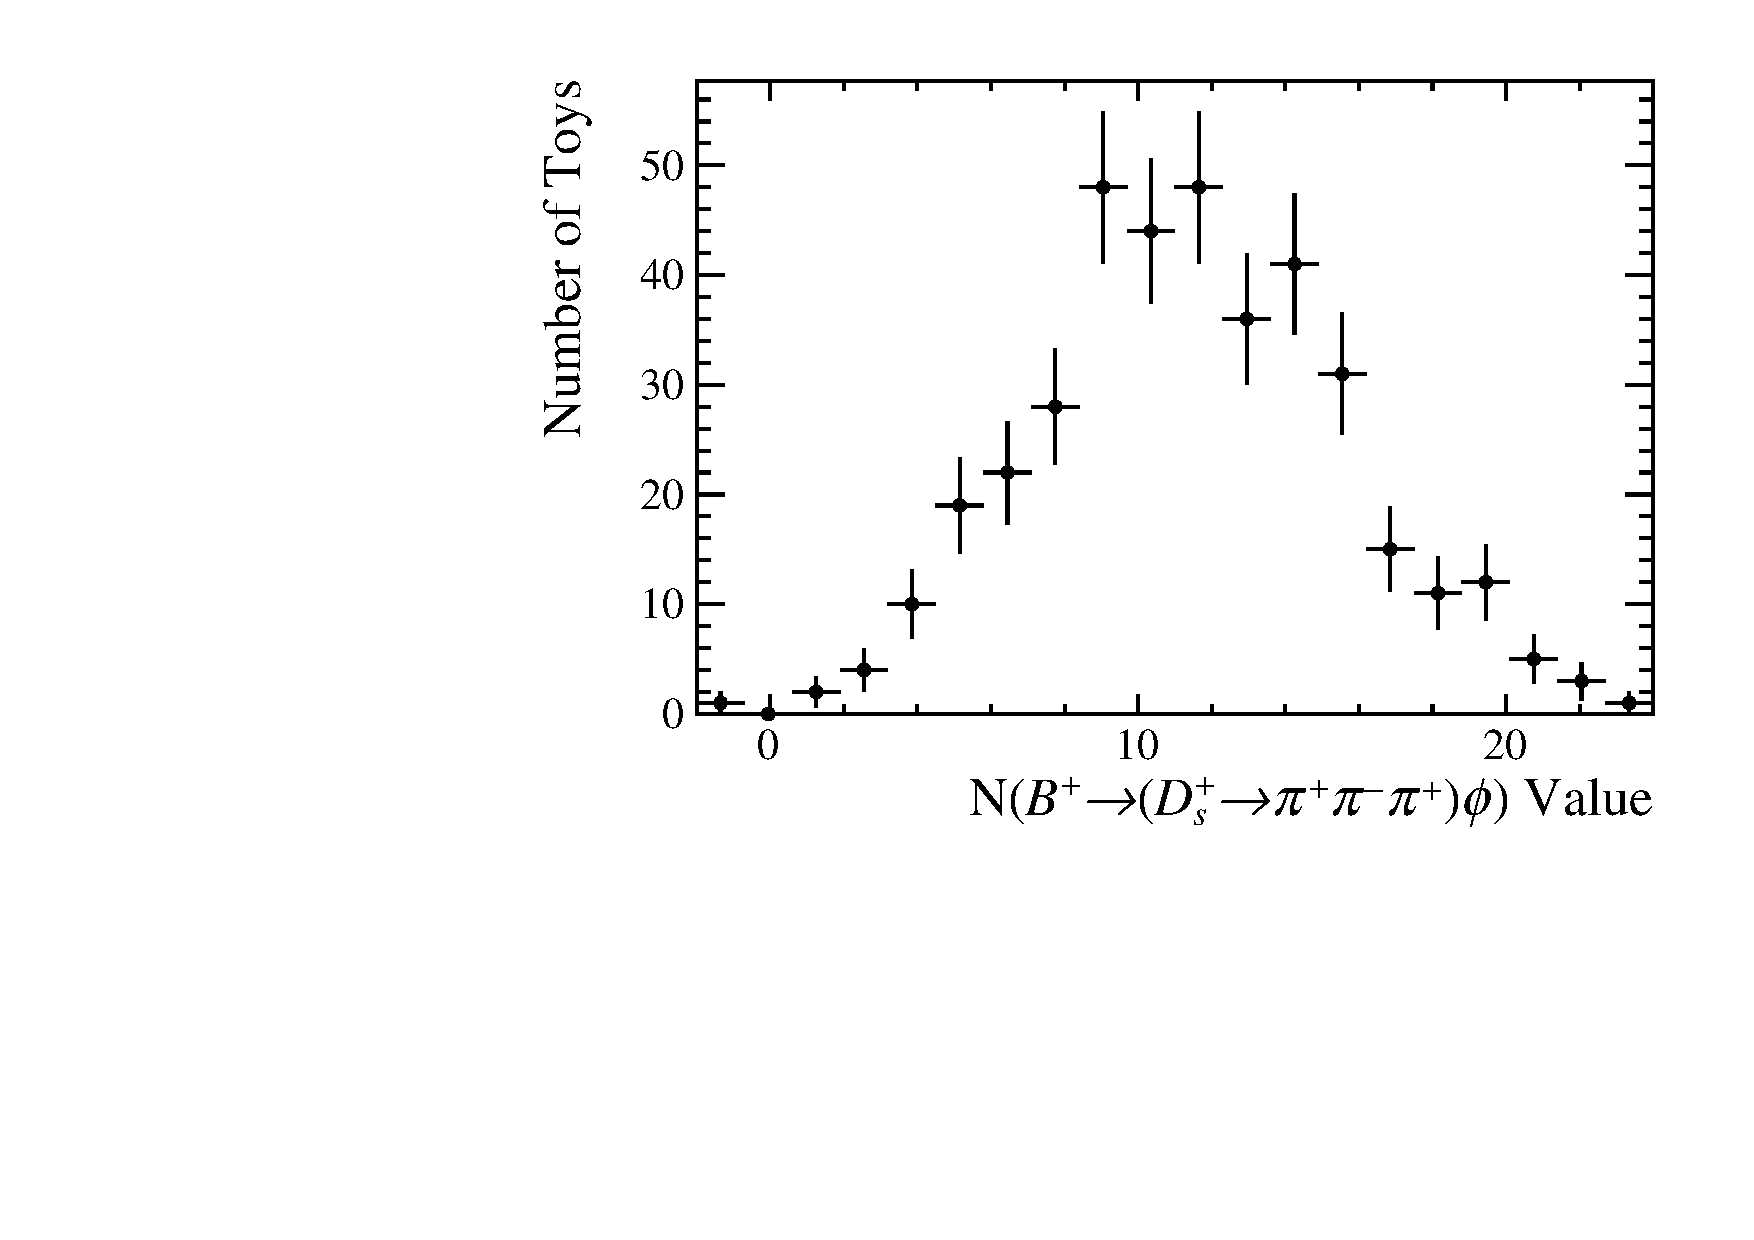
\includegraphics[width=0.32\textwidth]{figs/B2DsPhi/Plots_DsKK_Value_yield_peak_total_DsPhi_Ds2PiPiPi_toy_both_DsBDTbin1_PhiBDTbin1_both_both.pdf}
      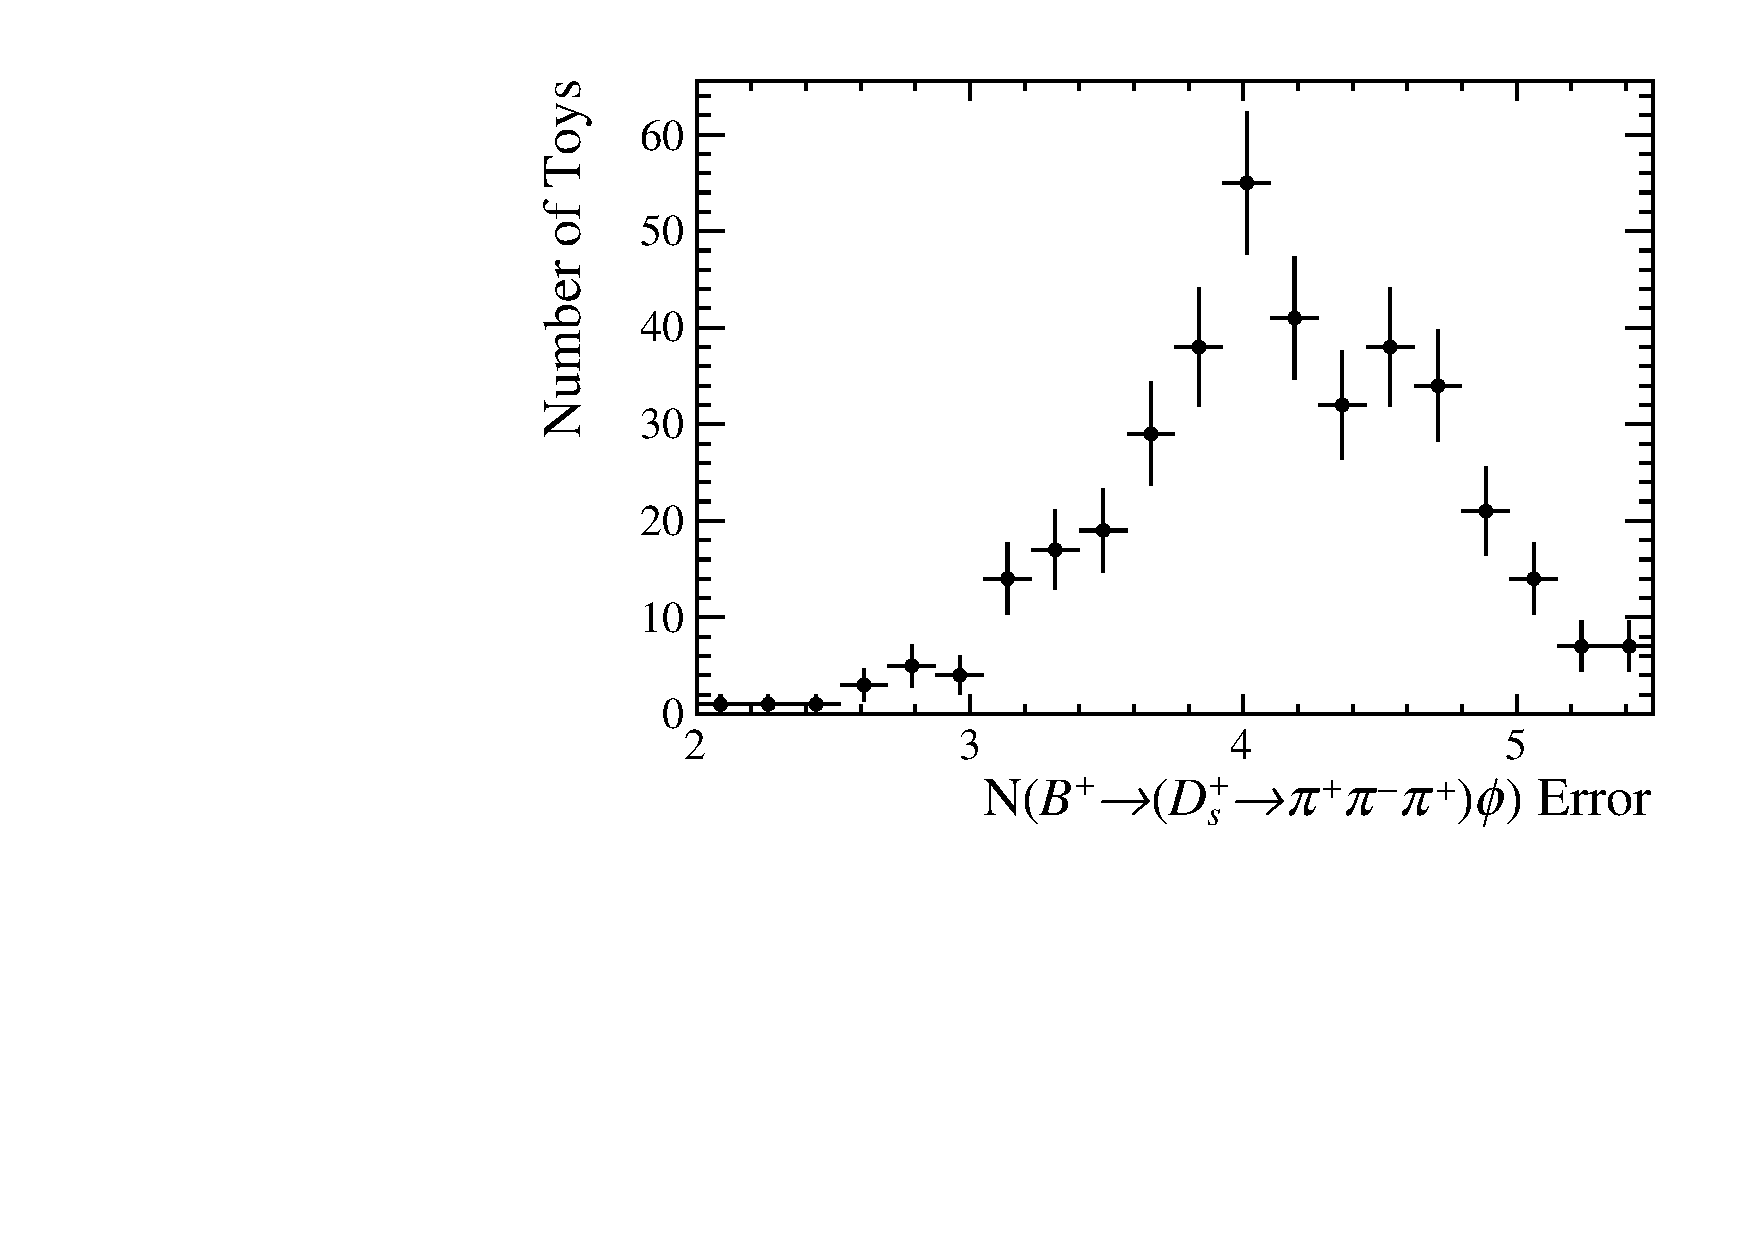
\includegraphics[width=0.32\textwidth]{figs/B2DsPhi/Plots_DsKK_Error_yield_peak_total_DsPhi_Ds2PiPiPi_toy_both_DsBDTbin1_PhiBDTbin1_both_both.pdf}
      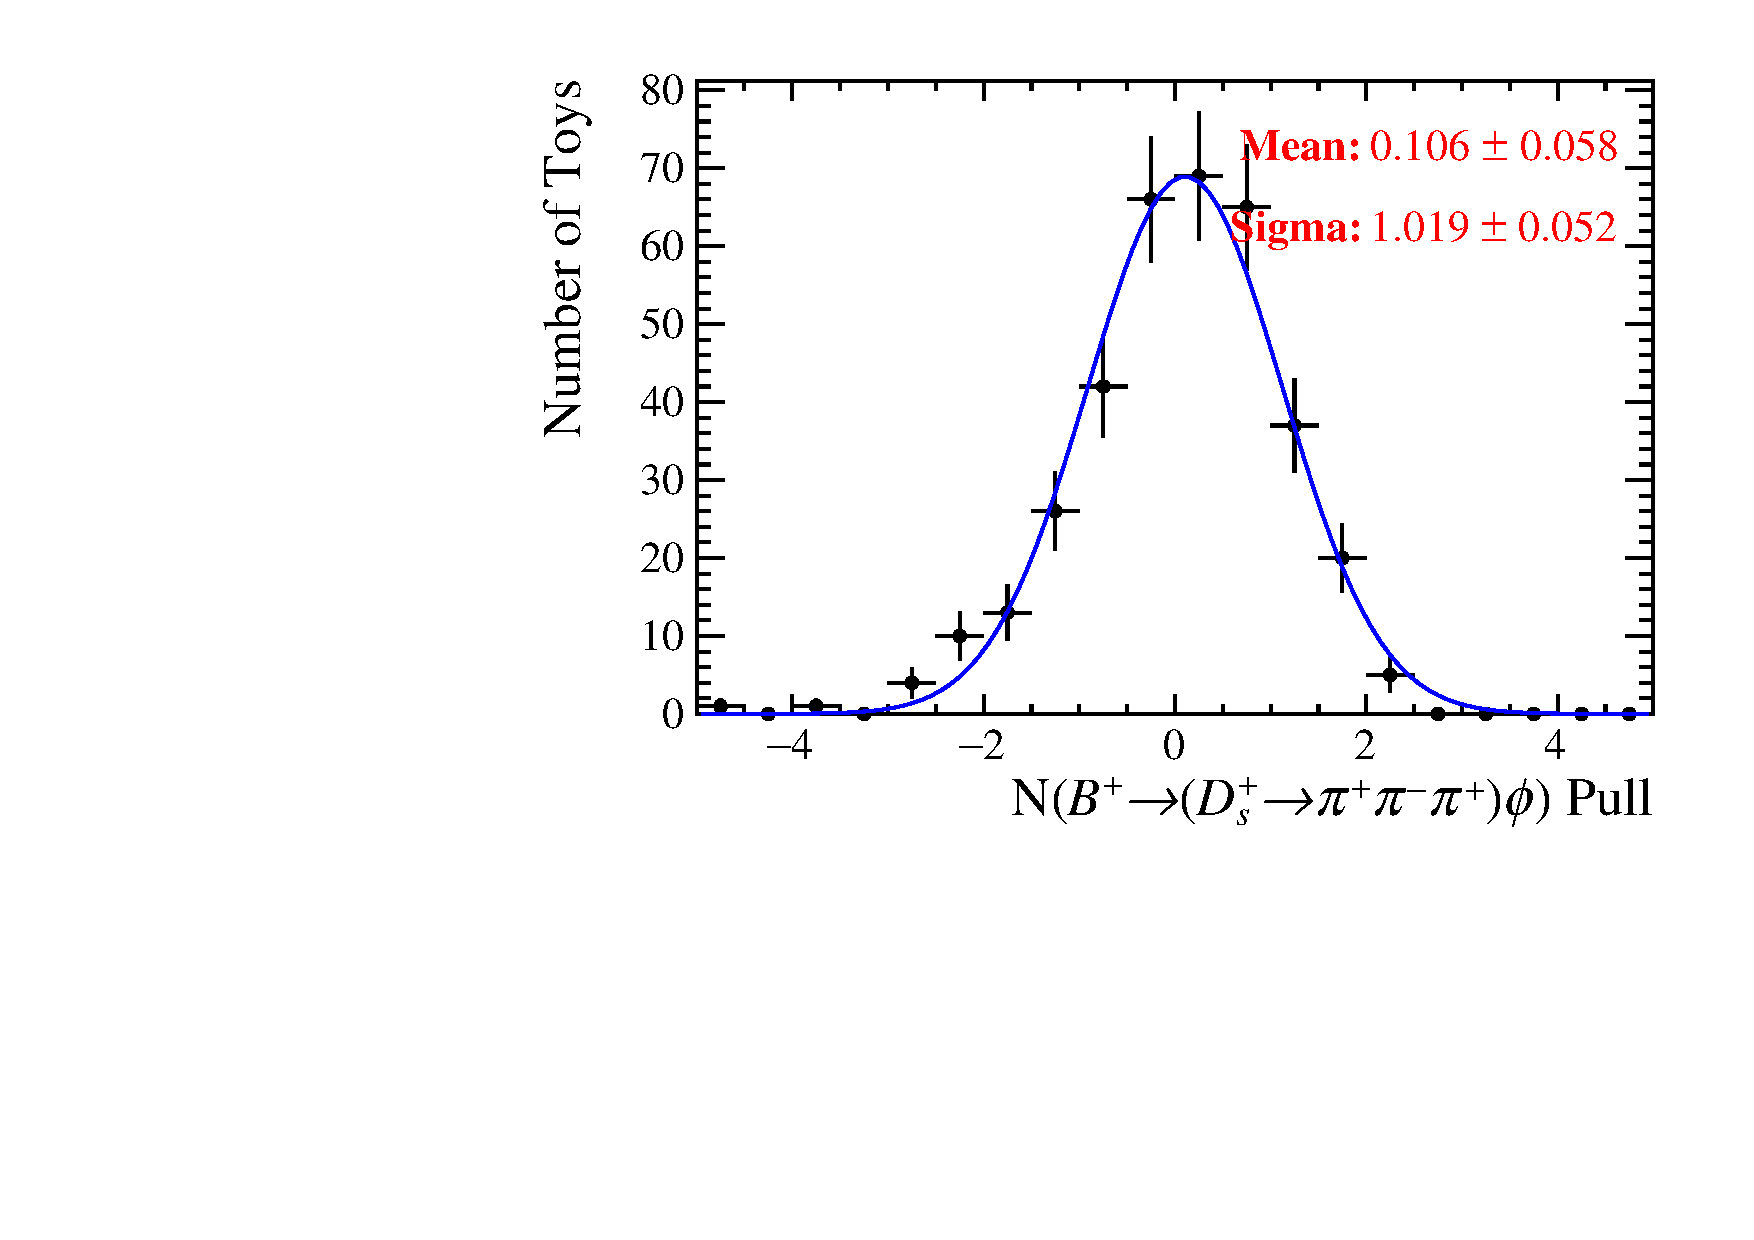
\includegraphics[width=0.32\textwidth]{figs/B2DsPhi/Plots_DsKK_Pull_yield_peak_total_DsPhi_Ds2PiPiPi_toy_both_DsBDTbin1_PhiBDTbin1_both_both.pdf}
      \caption{\decay{\Dsp}{\pip\pim\pip}}
   \end{subfigure}\\
   \begin{subfigure}[t]{1.0\textwidth}
      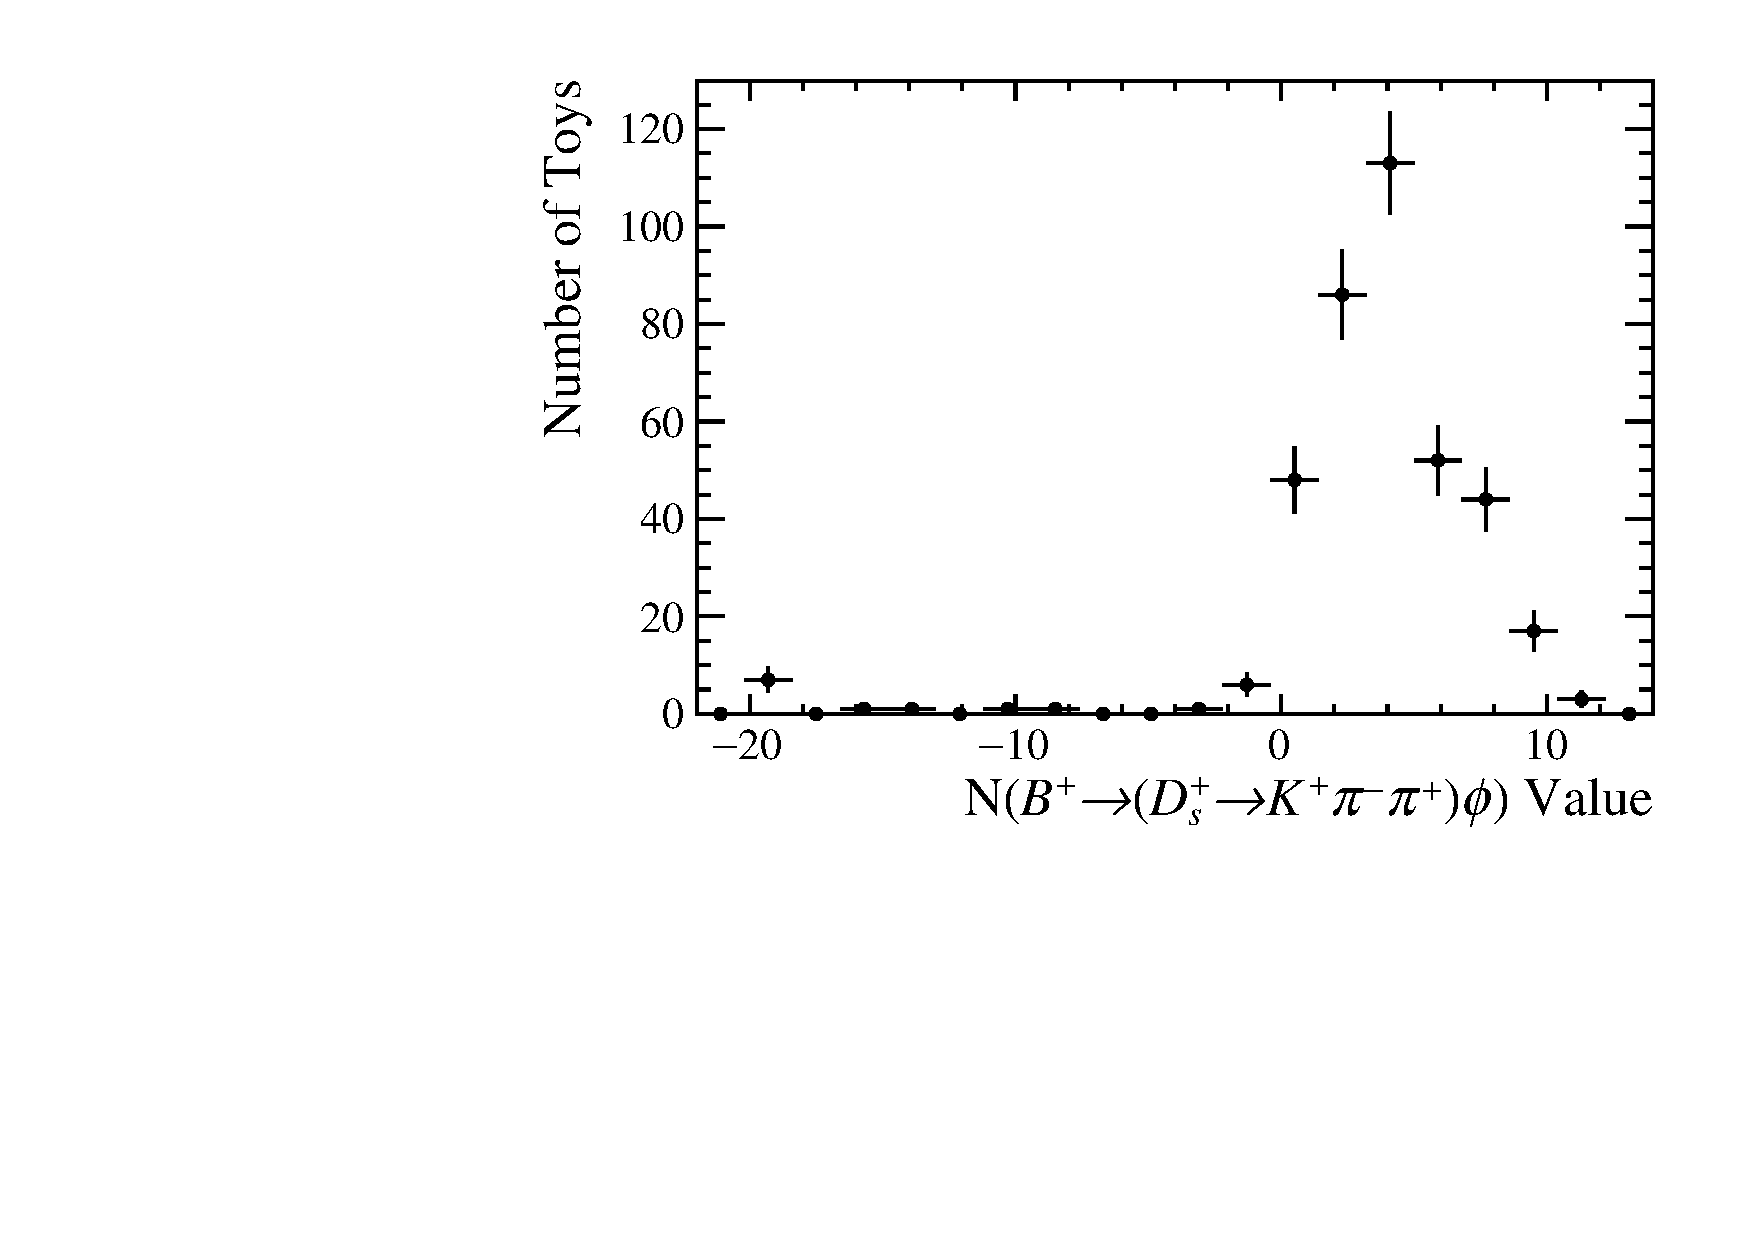
\includegraphics[width=0.32\textwidth]{figs/B2DsPhi/Plots_DsKK_Value_yield_peak_total_DsPhi_Ds2KPiPi_toy_both_DsBDTbin1_PhiBDTbin1_both_both.pdf}
      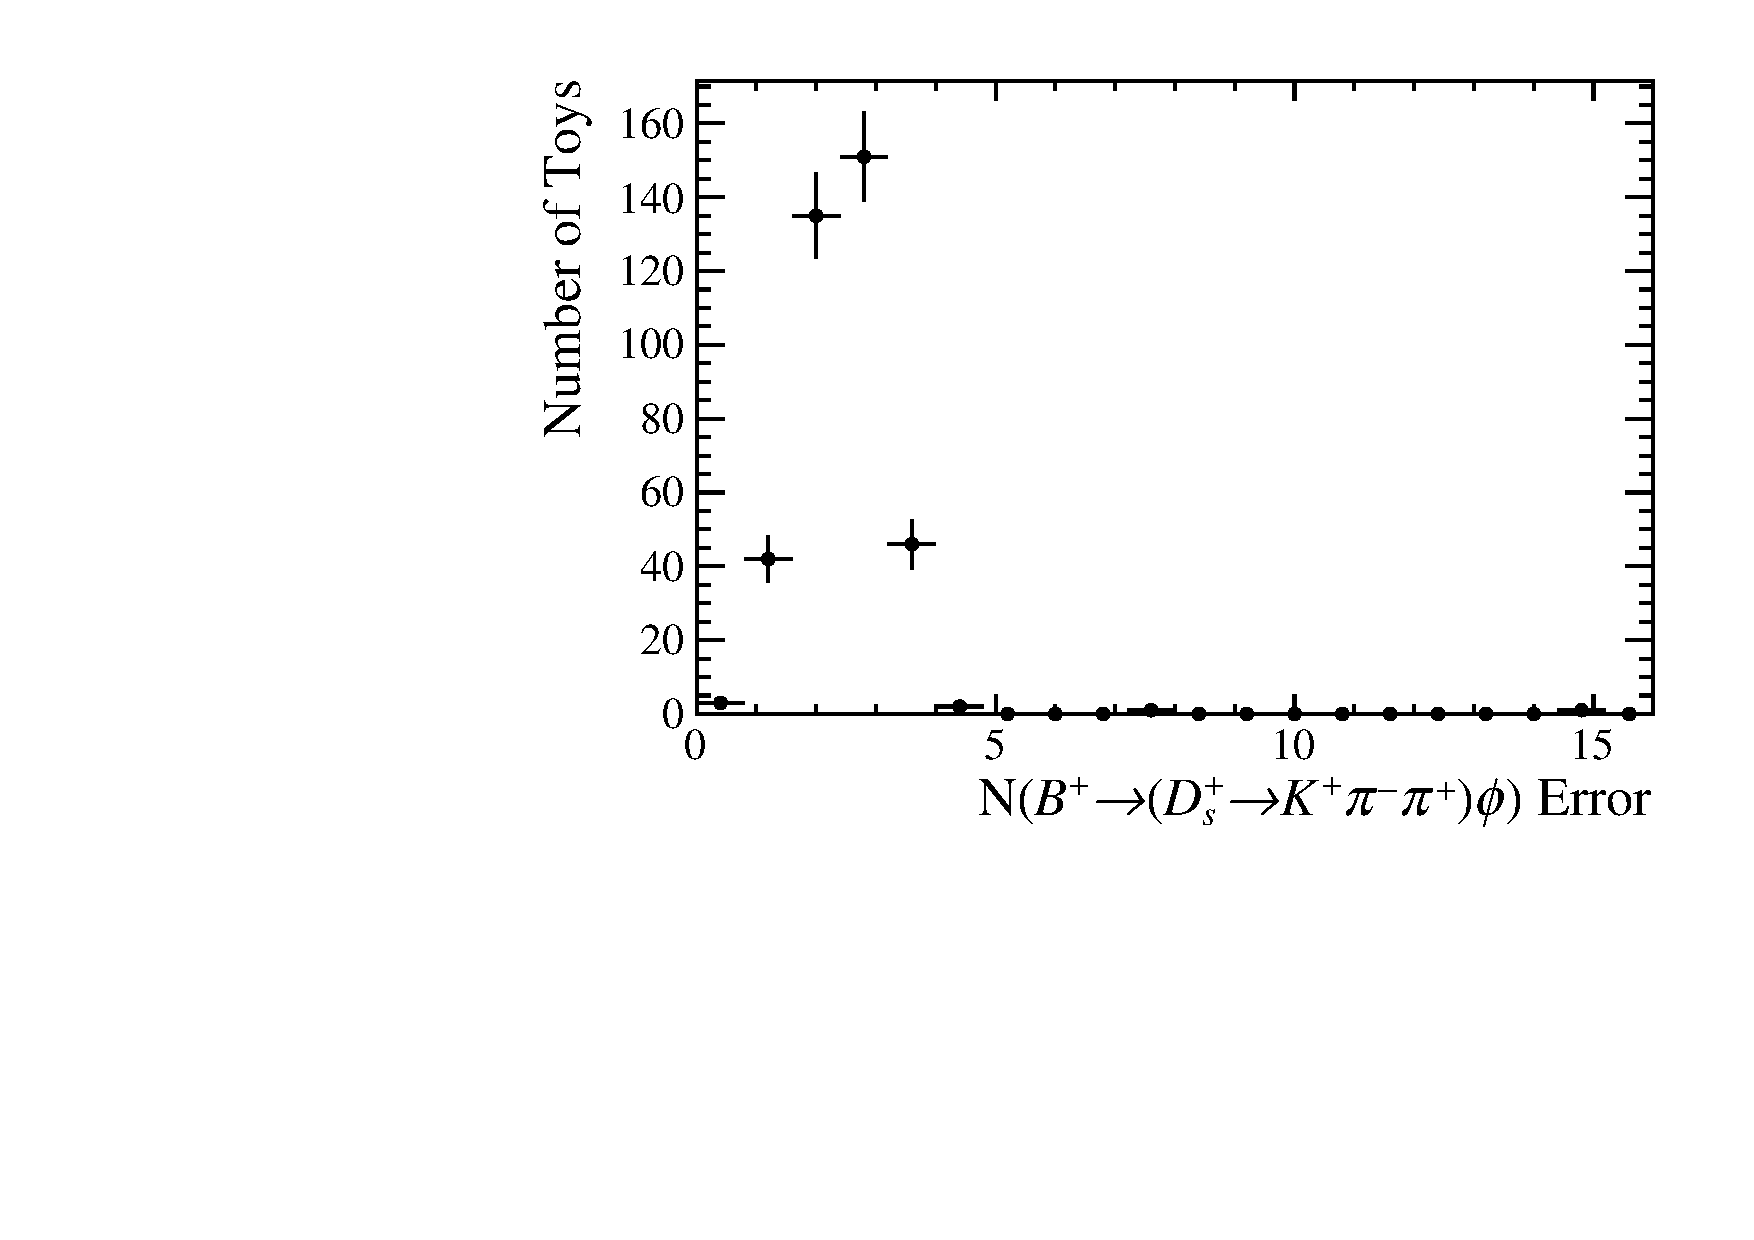
\includegraphics[width=0.32\textwidth]{figs/B2DsPhi/Plots_DsKK_Error_yield_peak_total_DsPhi_Ds2KPiPi_toy_both_DsBDTbin1_PhiBDTbin1_both_both.pdf}
      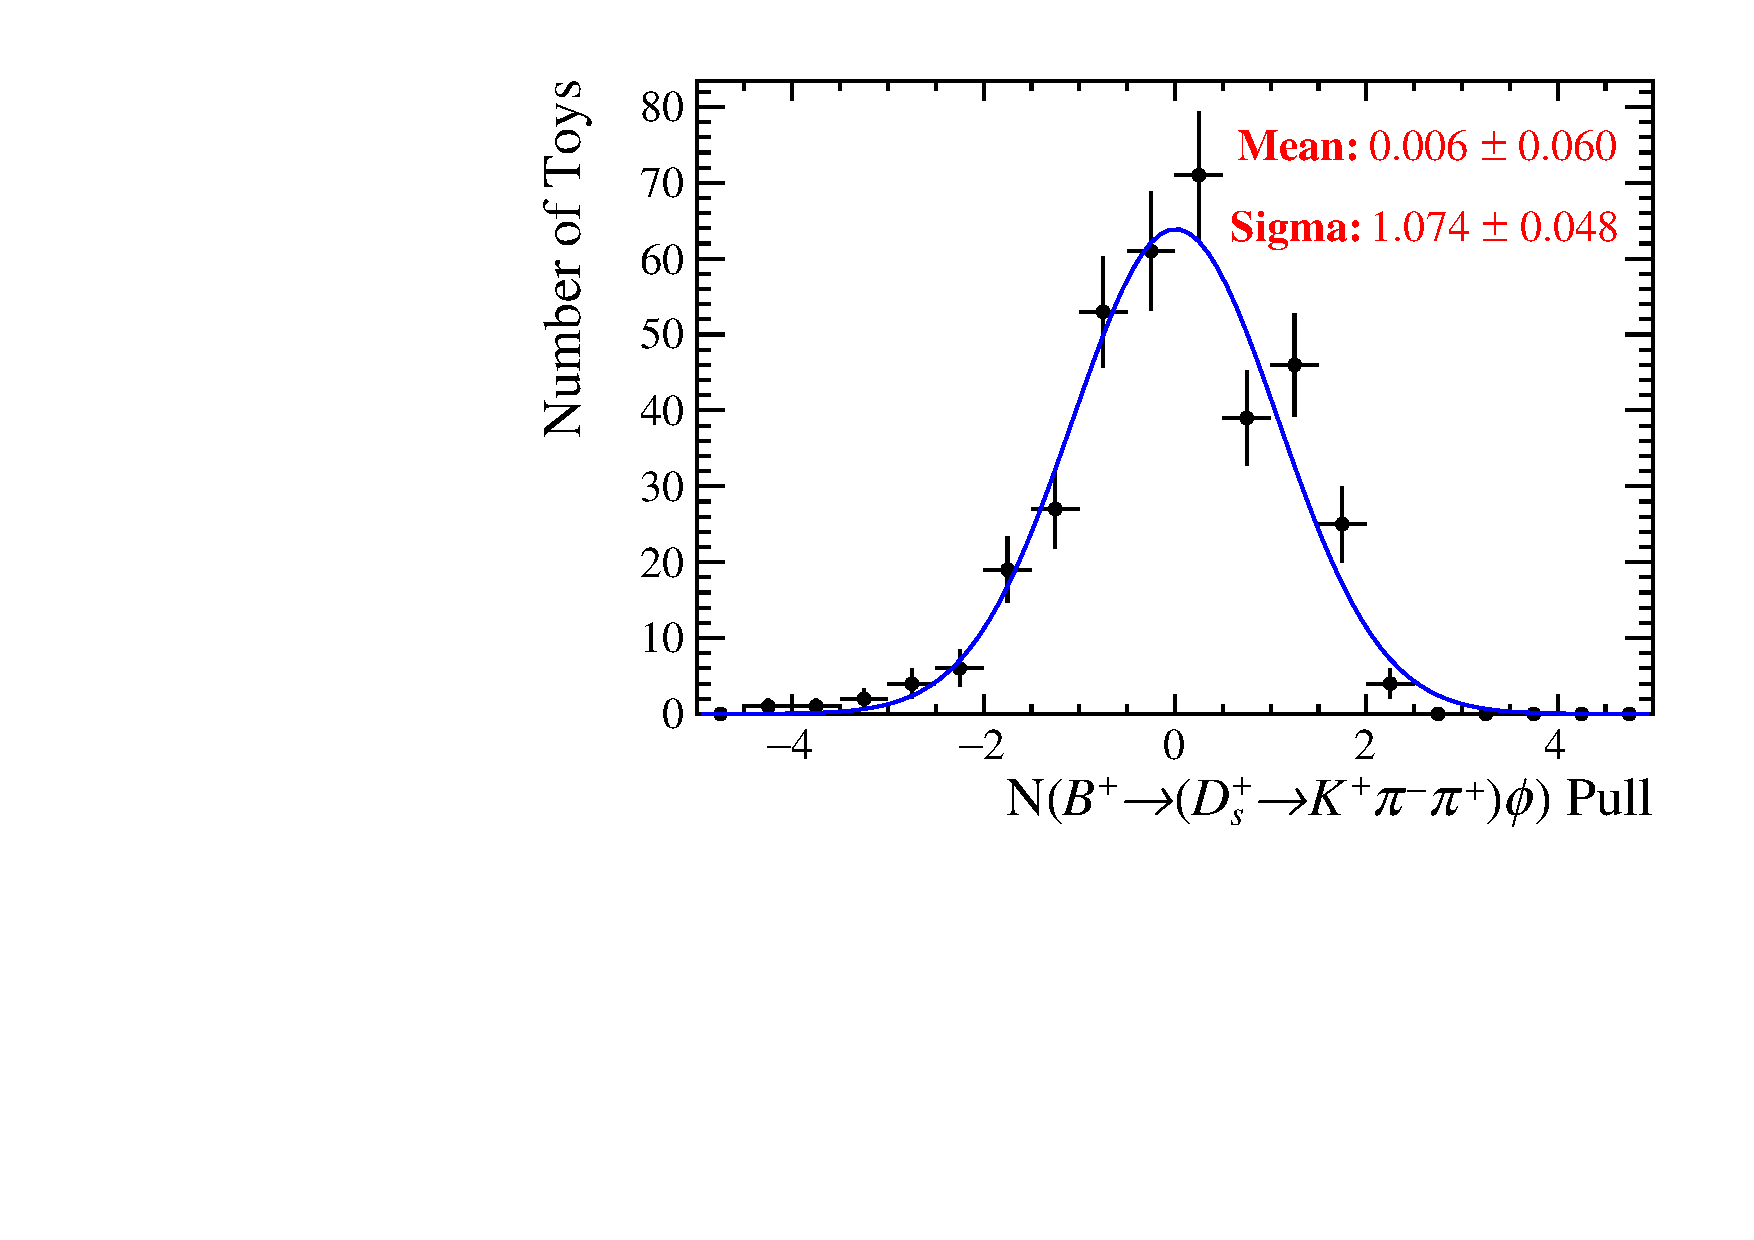
\includegraphics[width=0.32\textwidth]{figs/B2DsPhi/Plots_DsKK_Pull_yield_peak_total_DsPhi_Ds2KPiPi_toy_both_DsBDTbin1_PhiBDTbin1_both_both.pdf}
      \caption{\decay{\Dsp}{\Kp\pim\pip}}
   \end{subfigure}

   \caption{The yield, error and pull distributions for the signal channel.}
   \label{fig:B2DsPhi_Pulls_signal}
\end{figure}
%%%%%%%%%%%%%%%%%%%%%%%%%%%%%%%%%%%%%%%%%%%%%%%%%%%%%%%%%%

These distributions were generated using pseudo-experiments in which the yields for each \Dsp mode were free variables rather than being determined using a single free branching fraction parameter.

The model is also studied using a single branching fraction $\BF(\decay{\Bp}{\Dsp\phiz})$ that determines the yields in each signal mode. This parameter is calculated directly in the fit so it can be assessed for any possible bias. The distribution of the measured values, uncertainties and pulls are shown in Fig.~\ref{fig:B2DsPhi_Pulls_BR}.


%%%%%%%%%%%%%%%%%%%%%%%%%%%%%%%%%%%%%%%%%%%%%%%%%%%%%%%%%%
\begin{figure}[!h]
   \centering
   \begin{subfigure}[t]{1.0\textwidth}
      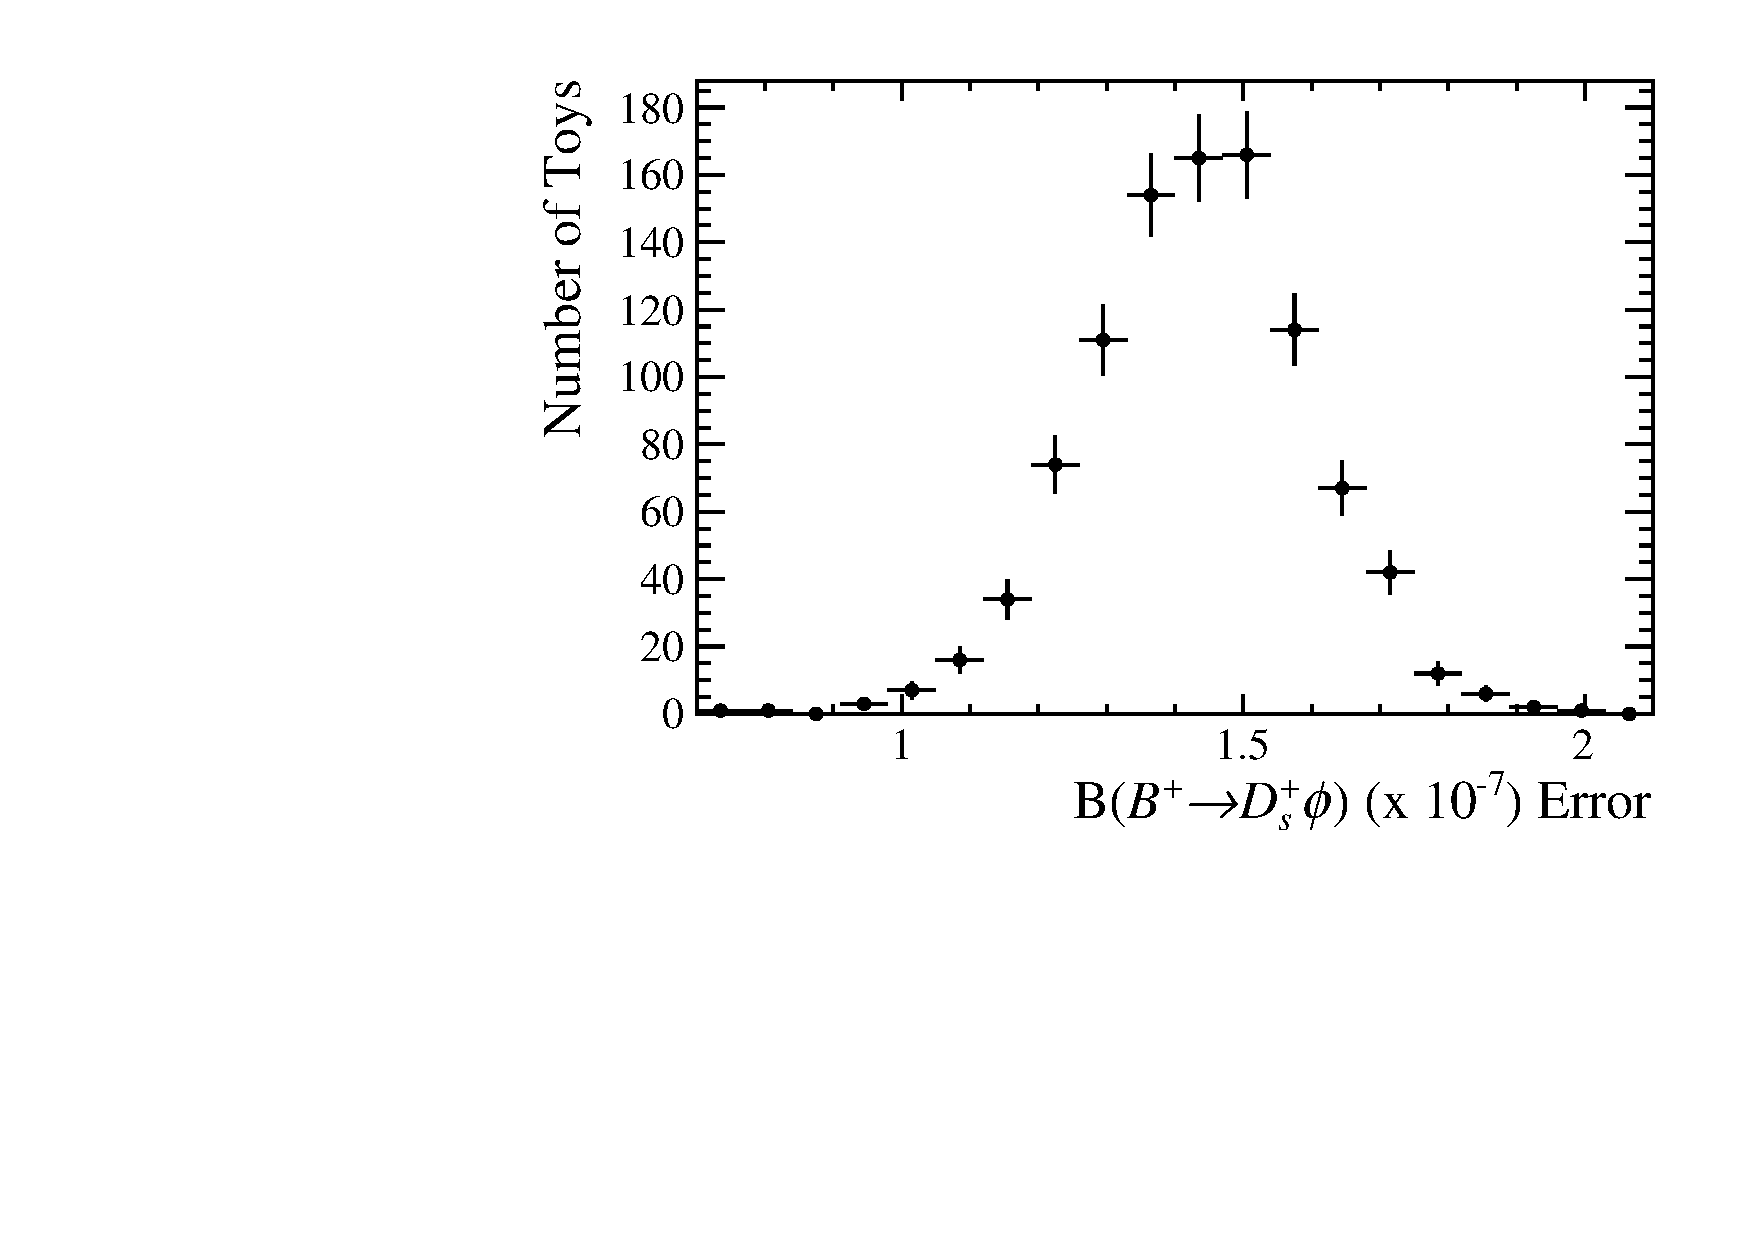
\includegraphics[width=0.32\textwidth]{figs/B2DsPhi/Plots_DsKK_Error_Branching_fraction.pdf}
      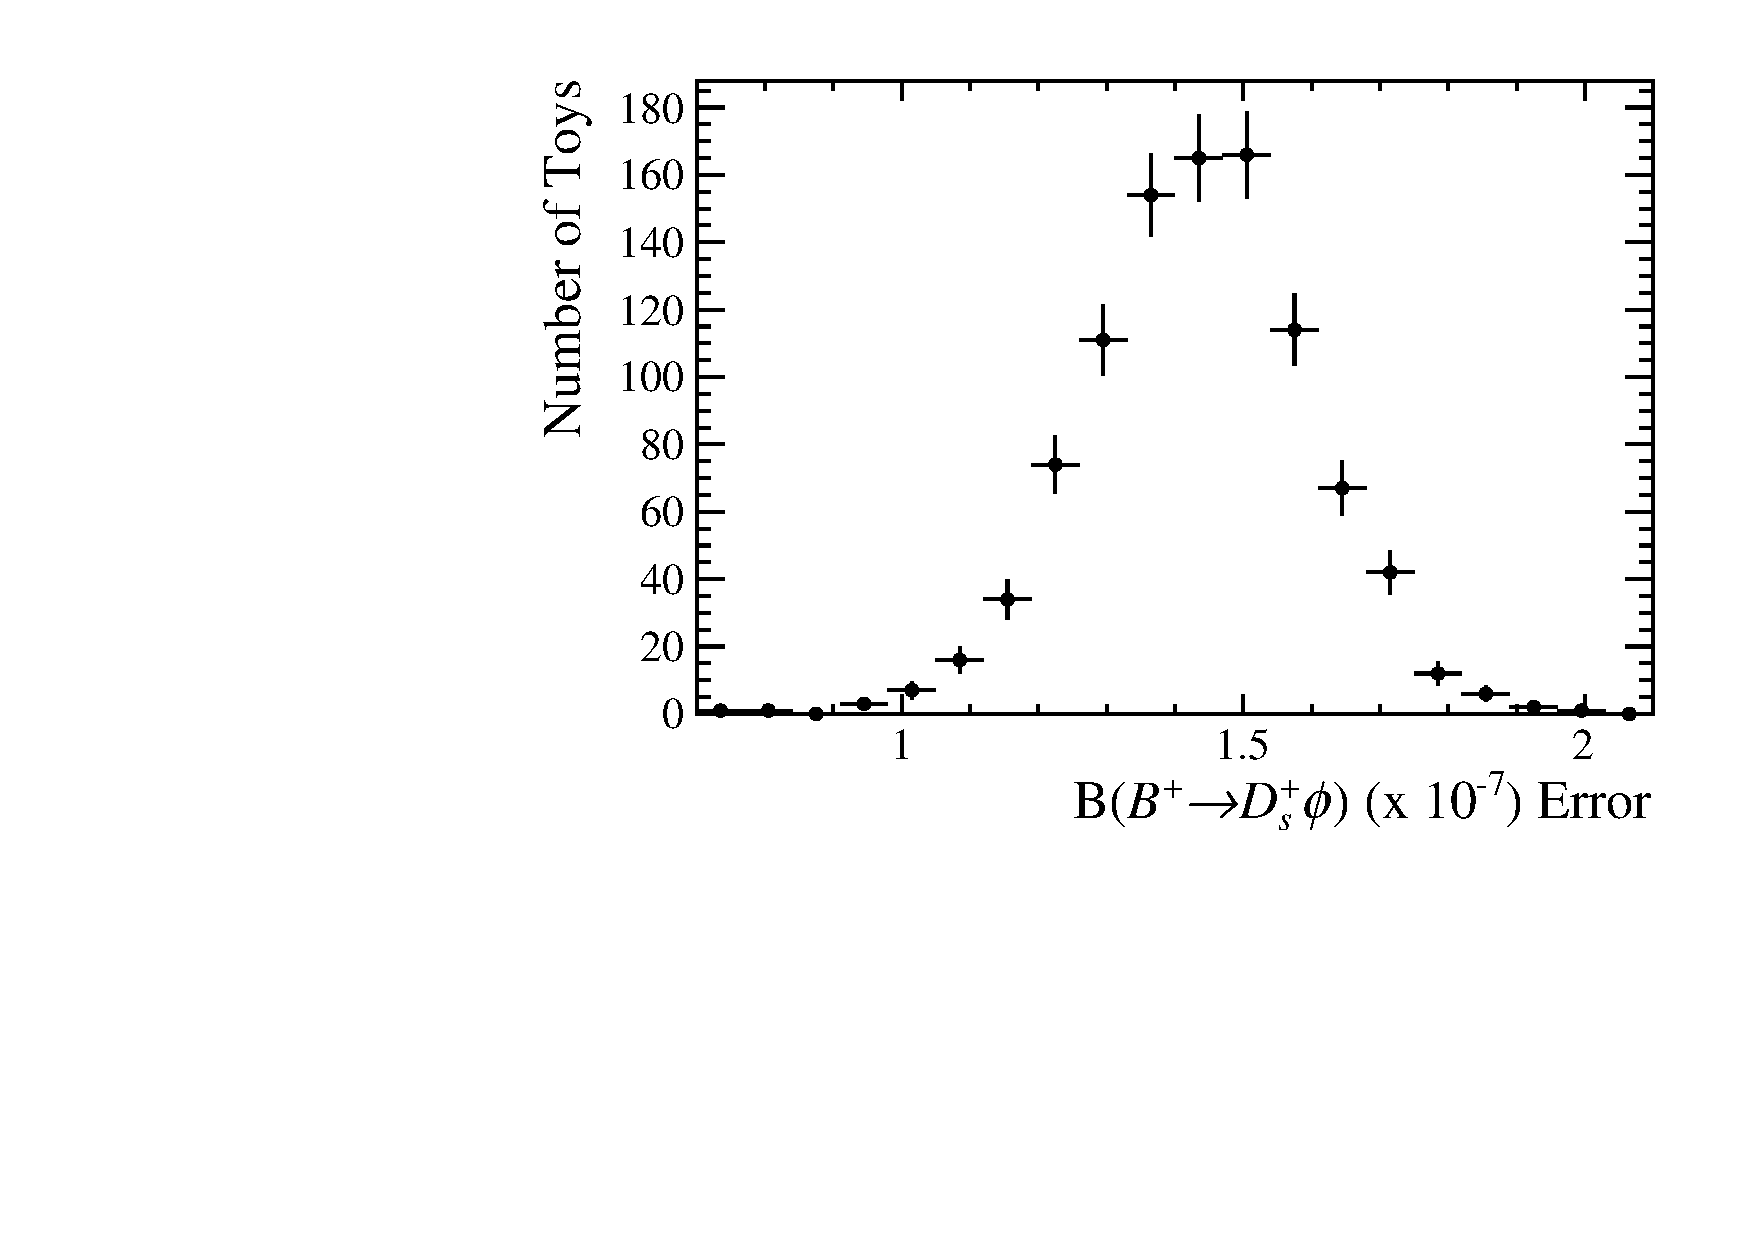
\includegraphics[width=0.32\textwidth]{figs/B2DsPhi/Plots_DsKK_Error_Branching_fraction.pdf}
      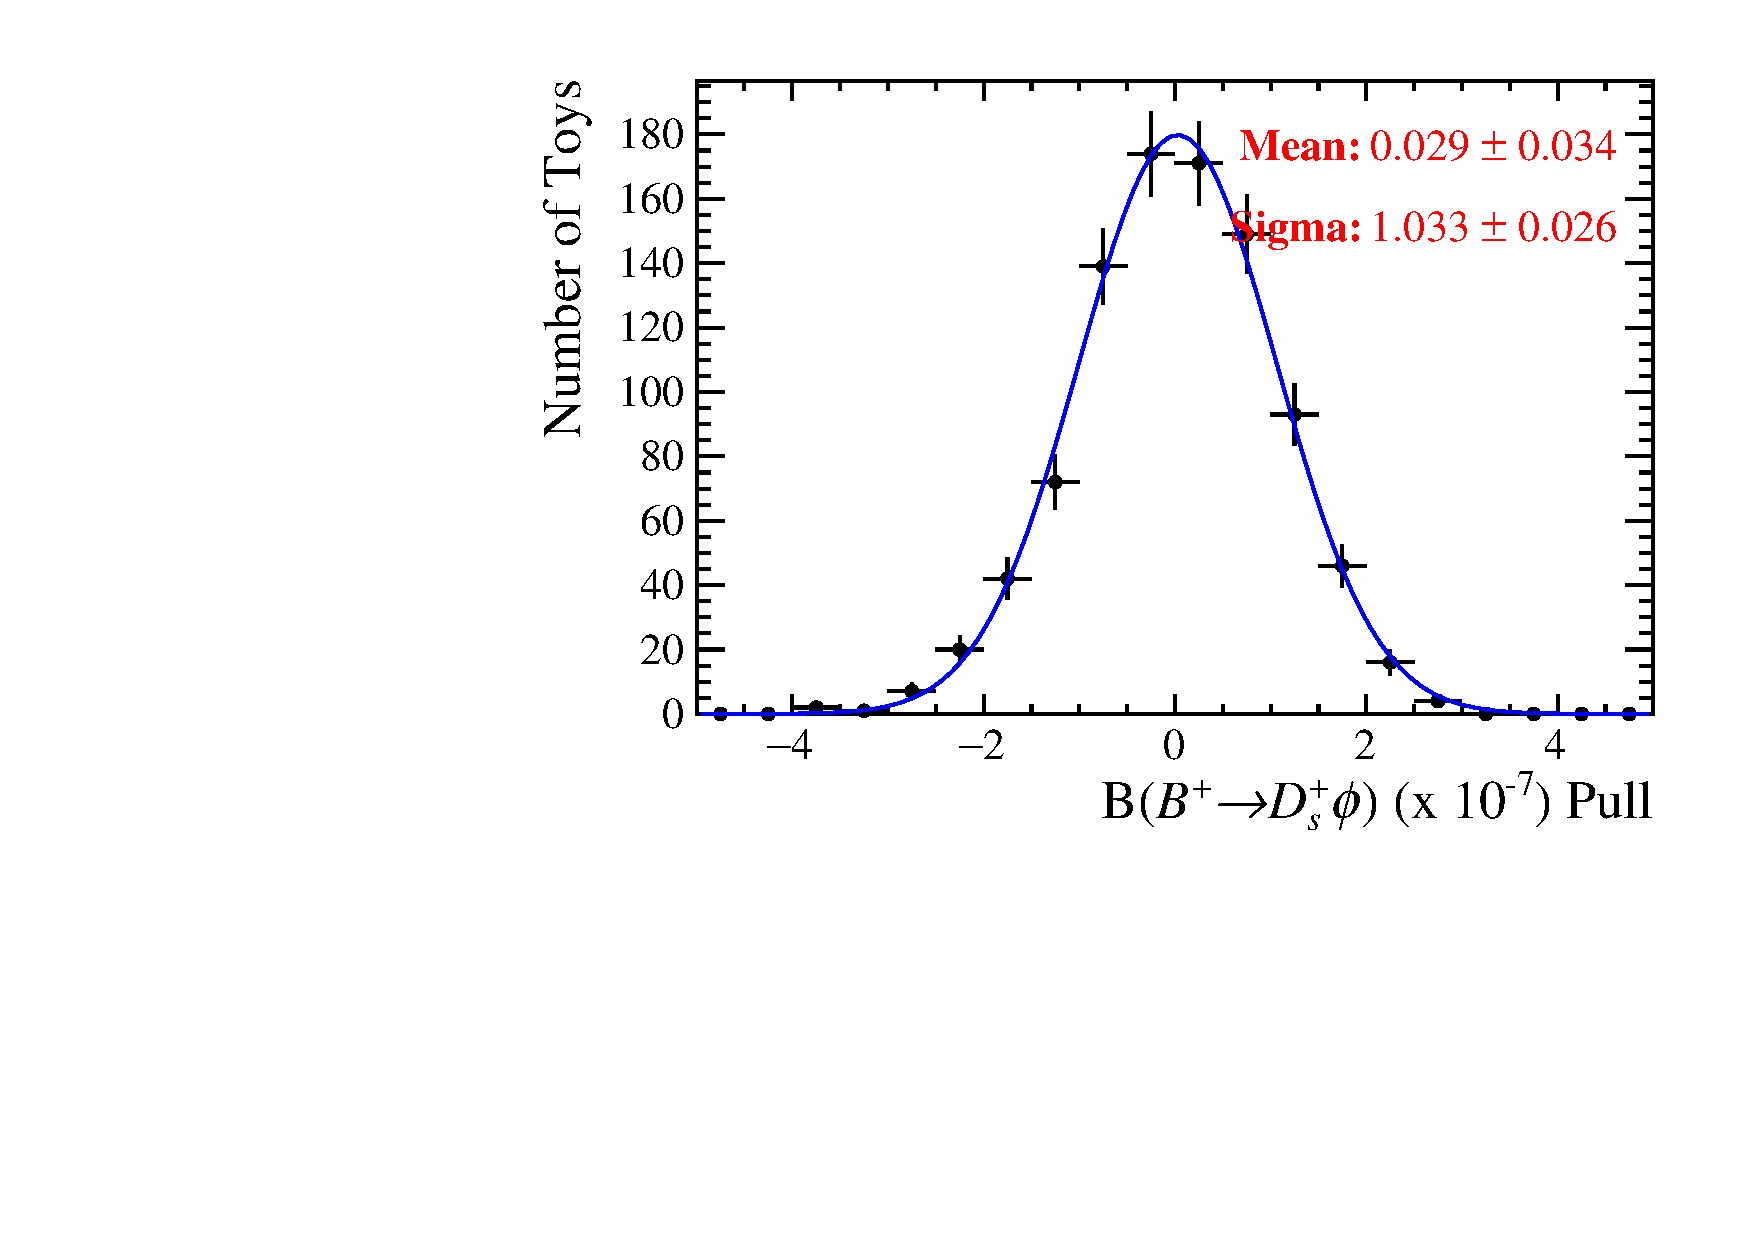
\includegraphics[width=0.32\textwidth]{figs/B2DsPhi/Plots_DsKK_Pull_Branching_fraction.pdf}
   \end{subfigure}
   \caption{The branching fraction, error and pull distributions for the full simultaneous fit. The branching fraction is generated assuming the value obtained in the fit to data.}
   \label{fig:B2DsPhi_Pulls_BR}
\end{figure}
%%%%%%%%%%%%%%%%%%%%%%%%%%%%%%%%%%%%%%%%%%%%%%%%%%%%%%%%%%
The pull mean and width are both within $2\sigma$ of zero and one respectively. 
As no significant biases are observed in the pulls of any of the yields or branching fraction no corrections are applied to the values determined fit.